%%%%%%%%%%%%%%%%%%%%%%%%%%%%%%%%%%%%%%%%%%%%%%%%%%%%%%
\section{Welcome to Condor}  
%
% .... or alternatively called the 'warm fuzzies' section
% <smirk>  
% 
%
% Warning: much of what you are about to read was very 
% hastily written by a very tired Todd.... Good Luck.  
%%%%%%%%%%%%%%%%%%%%%%%%%%%%%%%%%%%%%%%%%%%%%%%%%%%%%

\index{Condor!user manual|(}
\index{user manual|(}
Presenting Condor \VersionNotice! Condor is developed by
the Condor Team at the University of Wisconsin-Madison (UW-Madison), and
was first installed as a production system in the UW-Madison Computer
Sciences department nearly 10 years ago. This Condor pool has since
served as a major source of computing cycles to UW faculty and students.
For many, it has revolutionized the role computing plays in their
research. An increase of one, and sometimes even two, orders of
magnitude in the computing throughput of a research organization can
have a profound impact on its size, complexity, and scope. Over the
years, the Condor Team has established collaborations with scientists
from around the world and has provided them with access to surplus
cycles (one of whom has consumed 100 CPU years!). Today, our
department's pool consists of more than 700 desktop UNIX workstations.
On a typical day, our pool delivers more than 500 CPU days to UW
researchers. Additional Condor pools have been established over the
years across our campus and the world. Groups of researchers, engineers,
and scientists have used Condor to establish compute pools ranging in
size from a handful to hundreds of workstations. We hope that Condor
will help revolutionize your compute environment as well.


%%%%%%%%%%%%%%%%%%%%%%%%%%%%%%%%%%%%%%%%%%%%%%%%%%%%%%%
\section{What does Condor do?}
%%%%%%%%%%%%%%%%%%%%%%%%%%%%%%%%%%%%%%%%%%%%%%%%%%%%%%%


In a nutshell, Condor is a specialized batch system 
\index{batch system}
for managing compute-intensive jobs.
Like most batch systems, Condor provides a
queueing mechanism, scheduling policy, priority scheme, and resource
classifications.  Users submit their compute jobs to Condor, Condor puts
the jobs in a queue, runs them, and then informs the user as to the
result.

Batch systems normally operate only with dedicated machines.  Often 
termed compute servers, these dedicated machines are typically owned by
one organization and dedicated to the sole purpose of running compute
jobs.  Condor can schedule jobs on dedicated machines.  But unlike traditional 
batch systems, Condor is also designed to effectively 
utilize non-dedicated machines to run jobs.  By being told to only
run compute jobs on machines which are currently not being used (no keyboard
activity, no load average, no active telnet users, etc), Condor can
effectively harness otherwise idle machines throughout a pool of machines.
This is important because often times the amount of
compute power represented by the aggregate total of all the non-dedicated 
desktop workstations sitting on people's desks throughout the
organization is far greater than the compute power of a dedicated
central resource.

Condor has several unique capabilities at its disposal which are geared 
towards effectively utilizing non-dedicated resources that are not owned or
managed by a centralized resource. These include transparent process
checkpoint and migration, remote system calls, and ClassAds.
Read section~\ref{sec:what-is-condor} for a general 
discussion of these features before reading any further.


%%%%%%%%%%%%%%%%%%%%%%%%%%%%%%%%%%%%%%%%%%%%%%%%%%%%%%%%
\section{Condor Matchmaking with ClassAds}
%%%%%%%%%%%%%%%%%%%%%%%%%%%%%%%%%%%%%%%%%%%%%%%%%%%%%%%%

Before you learn about how to submit a job, it is important to
understand how Condor allocates resources. 
\index{Condor!resource allocation}
Understanding the
unique framework by which Condor matches submitted jobs with machines is
the key to getting the most from Condor's scheduling algorithm. 

Condor simplifies job submission by acting as a matchmaker of ClassAds.
Condor's ClassAds
\index{ClassAd}
are analogous to the classified advertising section of the
newspaper. Sellers advertise specifics about what they have to sell,
hoping to attract a buyer. Buyers may advertise specifics about what
they wish to purchase. Both buyers and sellers list constraints that
need to be satisfied.
For instance, a buyer has a maximum spending limit, 
and a seller requires a minimum purchase price.
Furthermore, both want to rank requests to their own advantage.
Certainly a seller would rank
one offer of \$50 dollars higher than a different
offer of \$25.
In Condor, users submitting
jobs can be thought of as buyers of compute resources and machine owners
are sellers. 

All machines in a Condor pool advertise their attributes,
\index{ClassAd!attributes}
such as
available RAM memory, CPU type and speed, virtual memory size, current
load average, along with other static and dynamic properties.
This machine ClassAd
\index{ClassAd!machine}
also advertises under what conditions it is
willing to run a Condor job and what type of job it would prefer. These
policy attributes can reflect the individual terms and preferences by
which all the different owners have graciously allowed their machine to
be part of the Condor pool. 
You may
advertise that your machine is only willing to run jobs at night
and when there is no keyboard activity on your machine.
In addition, you may
advertise a preference (rank) for running jobs submitted by you
or one of your co-workers. 

Likewise, when submitting a job, you specify a ClassAd with
your requirements and preferences.
The ClassAd
\index{ClassAd!job}
includes the
type of machine you  wish to use. For instance, perhaps you are
looking for the fastest floating point performance available.
You want Condor to rank available machines
based upon floating point performance. Or, perhaps you
care only that the machine has a minimum of 128 Mbytes of RAM.
Or, perhaps you will
take any machine you can get! These job attributes and requirements
are bundled up into a job ClassAd.

Condor plays the role of a matchmaker by continuously reading
all the job ClassAds and all the machine ClassAds, 
matching and ranking job ads with machine ads.
Condor makes certain that all
requirements in both ClassAds are satisfied. 

%%%%%
\subsection{Inspecting Machine ClassAds with \condor{status}}
%%%%%

\index{Condor commands!condor\_status}
Once Condor is installed,
you will get a feel for what
a machine ClassAd does by trying
the \Condor{status} command.
Try the \Condor{status} command to get
a summary of information from
ClassAds about the resources available in your pool.
Type \Condor{status} and hit enter to see a summary 
similar to the following:
\begin{center}
\begin{verbatim}
Name       Arch     OpSys        State      Activity   LoadAv Mem  ActvtyTime

adriana.cs INTEL    SOLARIS251   Claimed    Busy       1.000  64    0+01:10:00
alfred.cs. INTEL    SOLARIS251   Claimed    Busy       1.000  64    0+00:40:00
amul.cs.wi SUN4u    SOLARIS251   Owner      Idle       1.000  128   0+06:20:04
anfrom.cs. SUN4x    SOLARIS251   Claimed    Busy       1.000  32    0+05:16:22
anthrax.cs INTEL    SOLARIS251   Claimed    Busy       0.285  64    0+00:00:00
astro.cs.w INTEL    SOLARIS251   Claimed    Busy       0.949  64    0+05:30:00
aura.cs.wi SUN4u    SOLARIS251   Owner      Idle       1.043  128   0+14:40:15
\end{verbatim}
\Dots 
\end{center}


The \Condor{status} command has options that summarize machine ads 
in a variety of ways.
For example,
\begin{description}
\item[\Condor{status -available}] shows only machines which are
willing to run jobs now. 
\item[\Condor{status -run}] shows only machines
which are currently running jobs.  
\item[\Condor{status -l}] lists the machine ClassAds for all machines
in the pool.
\end{description}

Refer to the \Condor{status} command 
reference page located on page~\pageref{man-condor-status}
for a complete description of \Condor{status} command.

Figure~\ref{fig:CondorStatusL} shows the complete machine ad
\index{ClassAd!example}
\index{machine ClassAd}
for a single workstation: alfred.cs.wisc.edu. Some of the listed
attributes are used by
Condor for scheduling. Other attributes are for information purposes.
An important point is that \emph{any} of the attributes in a
machine ad can be utilized at job submission time as part of a request
or preference on what machine to use. Additional attributes
can be easily added. For example, your site administrator can
add a physical location attribute to your machine ClassAds.

%
% figures for this section
%
% condor_status -l alfred
%
\begin{center}
\begin{figure}
\CondorVerySmall
\begin{verbatim}
MyType = "Machine"
TargetType = "Job"
Name = "alfred.cs.wisc.edu"
Machine = "alfred.cs.wisc.edu"
StartdIpAddr = "<128.105.83.11:32780>"
Arch = "INTEL"
OpSys = "SOLARIS251"
UidDomain = "cs.wisc.edu"
FileSystemDomain = "cs.wisc.edu"
State = "Unclaimed"
EnteredCurrentState = 892191963
Activity = "Idle"
EnteredCurrentActivity = 892191062
VirtualMemory = 185264
Disk = 35259
KFlops = 19992
Mips = 201
LoadAvg = 0.019531
CondorLoadAvg = 0.000000
KeyboardIdle = 5124
ConsoleIdle = 27592
Cpus = 1
Memory = 64
AFSCell = "cs.wisc.edu"
START = LoadAvg - CondorLoadAvg <= 0.300000 && KeyboardIdle > 15 * 60
Requirements = TRUE
Rank = Owner == "johndoe" || Owner == "friendofjohn" 
CurrentRank =  - 1.000000
LastHeardFrom = 892191963
\end{verbatim}
\normalsize
\caption{\label{fig:CondorStatusL}Sample output from \Condor{status -l alfred}}
\end{figure}
\end{center}


%%%%%%%%%%%%%%%%%%%%%%%%%%%%%%%%%%%%%%%%%%%%%%%%%%%%%%%%%%%%%
\section{Road-map for running jobs with Condor}
%%%%%%%%%%%%%%%%%%%%%%%%%%%%%%%%%%%%%%%%%%%%%%%%%%%%%%%%%%%%%

\index{job!preparation}
The road to using Condor effectively is a short one.  The basics
are quickly and easily learned.

Here are all the steps needed to run a job using Condor.
\begin{description}

\item[Code Preparation.]
A job run under Condor must be able to 
run as a background batch job.
\index{job!batch ready}
Condor runs the program unattended and in the background. 
A program that runs in the background will not be able
to do interactive input and output.
Condor can redirect console output (stdout and stderr)
and keyboard input (stdin)
to and from files for you.
Create any needed files that contain
the proper keystrokes needed for program input.
Make certain the program will run correctly with the files.

\item[The Condor Universe.]
Condor has five
runtime environments (called a \Term{universe}) from which to choose.
Of the five, two are likely choices when learning
to submit a job to Condor: the standard universe and the vanilla universe.
The standard universe allows a job running under Condor to
handle system calls by returning them to the machine where the
job was submitted.
The standard universe also provides the mechanisms necessary
to take a checkpoint and migrate a partially completed job,
should the machine on which the job is executing become
unavailable.
To use the standard universe, it is necessary to
relinking the program with the Condor library using the
\Condor{compile} command.
The manual page on page~\pageref{man-condor-submit} has details.

The vanilla universe provides a way to run jobs that cannot be
?.
It depends on a shared file system for access to input and output
files,
and there is no way to take a checkpoint or migrate a job executed
under the vanilla universe.

Choose a universe under which to run the Condor program,
and re-link the program if necessary.

\item[Submit description file.]
Controlling the details of a job submission is a
submit description file.
The file contains information
about the job such as what executable to run, the
files to use for keyboard and screen data,
the platform type required to run the program, and
where to send e-mail when the job completes.
You can also tell Condor how many times to run a program;
it is simple to run the same program
multiple times with multiple data sets.

Write a submit description file to go with the job, using
the examples provided in section~\ref{sec:sample-submit-files}
for guidance.

\item[Submit the Job.]Submit the program to Condor with
the \Condor{submit} command.
\index{Condor commands!condor\_submit}

\end{description}

Once submitted, Condor does the rest toward running
the job.
Monitor the job's progress with the \Condor{q}
\index{Condor commands!condor\_q}
and \Condor{status} commands.
\index{Condor commands!condor\_status}
You may modify the order in which Condor will run your jobs with
\Condor{prio}. If desired, Condor can even inform you in a log file 
every time your job is checkpointed and/or migrated to a different machine. 

When your program completes, Condor will tell you
(by e-mail, if preferred) the exit status of your program and various
statistics about its performances, including time used and I/O performed.
If you are using a log file for the job(which is recommended) the exit
status will be recorded in the log file.
You can remove a job from the
queue prematurely with \Condor{rm}. 
\index{Condor commands!condor\_rm}


%%%%%%%%%%%%%%%%%%%%%%%%%%%%%%%%%%%%%%%%%%%%%%%%
\subsection{\label{sec:Choosing-Universe}
Choosing a Condor Universe}
%%%%%%%%%%%%%%%%%%%%%%%%%%%%%%%%%%%%%%%%%%%%%%%%

A \Term{universe} in Condor
\index{universe}
\index{Condor!universe}
defines an execution environment. 
Condor \VersionNotice\ supports five different
universes for user jobs:
\begin{itemize}
	\item Standard
	\item Vanilla
	\item PVM
	\item MPI
	\item Globus
\end{itemize}

The \AdAttr{Universe} attribute is specified in the submit description file.
If the universe is not specified, then it will default to \Expr{standard}.

\index{universe!standard}
The \Expr{standard} universe provides migration and reliability, but has some
restrictions on the programs that can be run. 
\index{universe!vanilla}
The \Expr{vanilla} universe provides fewer services, but has very few
restrictions.
\index{universe!PVM}
The \Expr{PVM} universe is for programs written to the Parallel Virtual
Machine interface.  See section~\ref{sec:PVM} for more about PVM and Condor.
\index{universe!MPI}
The \Expr{MPI} universe is for programs written to the MPICH interface.
See section~\ref{sec:MPI} for more about MPI and Condor.
\index{universe!Globus}
The Globus universe allows users to submit Globus jobs through the
Condor interface.  See \Url{http://www.globus.org} for more about Globus.

%%%%%%%%%%%%%%%%%%%%%%%%%%%%%%%%%%%%%%%%%%%%%%%%%%%%%%%%%%%%%%%%%%%%%%
\subsubsection{\label{sec:standard-universe}Standard Universe}
%%%%%%%%%%%%%%%%%%%%%%%%%%%%%%%%%%%%%%%%%%%%%%%%%%%%%%%%%%%%%%%%%%%%%%

\index{universe!standard}
In the standard universe, Condor provides \Term{checkpointing} and
\Term{remote system calls}.  These features make a job more reliable
and allow it uniform access to resources from anywhere in the pool.
To prepare a program as a standard universe job, it must be re-linked
with \Condor{compile}.  Most programs can be prepared as a standard
universe job, but there are a few restrictions.

\index{checkpoint}
\index{checkpoint image}
Condor checkpoints a job at regular intervals.
A \Term{checkpoint image} is like a snapshot of the current
state of a job.  If a job must be migrated from one machine to another,
Condor makes a checkpoint image, copies the image to the new machine,
and restarts the job \emph{right where it left off}.  If a machine should
crash or fail while it is running a job, Condor can restart the job on
a new machine from the most recent checkpoint image.  In this way, jobs
can run for months or years even in the face of occasional computer failures.

\index{remote system call}
\index{shadow}
Remote system calls make a job perceive that it is executing on its home
machine, even though it may execute on many different machines over its
lifetime.  When your job runs on a remote machine, a second process, called
a \Condor{shadow} runs on the machine where you submitted the job.
\index{condor\_shadow}
\index{agents!condor\_shadow}
\index{Condor daemon!condor\_shadow}
\index{remote system call!condor\_shadow}
Whenever your job attempts a system call, the \Condor{shadow} performs
it instead and sends the results back.  So, if your job attempts to
open a file that is stored only on the submitting machine,
the \Condor{shadow} will find it and send the data to the machine where
your job happens to be running.

To convert your program into a standard universe job, you must use
\Condor{compile} to re-link it with the Condor libraries.  Simply
put \Condor{compile} in front of your usual link command.
You do not need to modify the program's source code,
but you do need access to its un-linked object files.  A commercial
program that is packaged as a single executable file cannot be
converted into a standard universe job.

For example, if you normally link your job by executing:
\begin{verbatim}
% cc main.o tools.o -o program
\end{verbatim}

Then you can re-link your job for Condor with:
\begin{verbatim}
% condor_compile cc main.o tools.o -o program
\end{verbatim}

There are a few restrictions on standard universe jobs:


\begin{enumerate}

\index{Unix!fork}
\index{Unix!exec}
\index{Unix!system}
\item Multi-process jobs are not allowed.  This includes system calls such as
\Syscall{fork}, \Syscall{exec}, and \Syscall{system}.

\index{Unix!pipe}
\index{Unix!semaphore}
\index{Unix!shared memory}
\item Interprocess communication is not allowed.  This includes pipes, semaphores, and shared memory.

\index{Unix!socket}
\index{network}
\item Network communication must be brief.  A job \emph{may} make network
connections using system calls such as \Syscall{socket}, but a network
connection left open for long periods will delay checkpointing and migration.

\index{signal}
\index{signal!SIGUSR2}
\index{signal!SIGTSTP}
\item Sending or receiving the SIGUSR2 or SIGTSTP signals is not allowed.
Condor reserves these signals for its own use.  Sending or receiving all
other signals \emph{is} allowed.

\index{Unix!alarm}
\index{Unix!timer}
\index{Unix!sleep}
\item Alarms, timers, and sleeping are not allowed.  This includes system
calls such as \Syscall{alarm}, \Syscall{getitimer}, and \Syscall{sleep}.

\index{thread!kernel-level}
\index{thread!user-level}
\item Multiple kernel-level threads are not allowed.  However,
multiple user-level threads \emph{are} allowed.

\index{file!memory-mapped}
\index{Unix!mmap}
\item Memory mapped files are not allowed.  This includes system calls such
as \Syscall{mmap} and \Syscall{munmap}.

\index{file!locking}
\index{Unix!flock}
\index{Unix!lockf}
\item File locks are allowed, but not retained between checkpoints.

\index{file!read only}
\index{file!write only}
\item All files must be opened read-only or write-only.  A file opened
for both reading and writing will cause trouble if a job must be rolled back
to an old checkpoint image.  For compatibility reasons, a file opened
for both reading and writing will result in a warning but not an error.

\item A fair amount of disk space must be available on the submitting machine
for storing a job's checkpoint images.  A checkpoint image is approximately
equal to the virtual memory consumed by a job while it runs.  If disk space
is short, a special \Term{checkpoint server} can be designated for storing
all the checkpoint images for a pool.

\index{linking!dynamic}
\index{linking!static}
\item On Linux, the job must be statically linked. 
\Condor{compile} does this by default.

\index{Unix!large files} 
\item Reading to or writing from files larger than 2 GB is only supported
when the submit side \Condor{shadow} and the standard universe user job
application itself are both 64-bit executables.

\end{enumerate}






%%%%%%%%%%%%
\subsubsection{Vanilla Universe}
%%%%%%%%%%%%

\index{universe!vanilla}
The vanilla universe in Condor is intended
for programs which cannot
be successfully re-linked.
Shell scripts are another case where the vanilla universe
is useful.
Unfortunately, jobs run under the vanilla universe cannot checkpoint or use
remote system calls. 
This has unfortunate consequences for a job that is partially
completed 
when the remote machine running a job must be returned
to its owner.
Condor has only two choices.  It can suspend the job, hoping to
complete it at a later time,
or it can give up and restart the job \emph{from the beginning} 
on another machine in the pool.

\Notice{
In UNIX, jobs submitted as vanilla universe jobs can only rely on an
external mechanism for accessing data files from different machines
such as NFS or AFS. The job \emph{must} be able to access your data
files on any machine on which it could potentially run. As an example,
suppose your work machine is blackbird.cs.wisc.edu and your job requires
a particular data file \File{/u/p/s/psilord/data.txt}. You wish to
submit to Condor from this machine and the job can potentially run on
cardinal.cs.wisc.edu. If the job runs on that machine, it must have
\File{/u/p/s/psilord/data.txt} available through either NFS or AFS for
your job to run correctly.

Condor deals with this restriction of the vanilla universe by
the \AdAttr{FileSystemDomain} and \AdAttr{UidDomain} machine
ClassAd attributes that reflect the reality of the pool's disk
mounting structure. If you have a large pool spanning multiple
\AdAttr{UidDomain} and/or \AdAttr{FileSystemDomain}s then you must specify
your \AdAttr{requirements} to use the correct \AdAttr{UidDomain} and/or
\AdAttr{FileSystemDomain}s that your jobs need to access your data
files.

However, under Windows NT, the vanilla universe \emph{does not} require
a shared file system due to the Condor File Transfer mechanism. Please see
chapter~\ref{condor-nt} for more details about Condor NT.
}

%%%%%%%%%%%%
\subsubsection{PVM}
%%%%%%%%%%%%

\index{universe!PVM}
The PVM universe allows programs written to the Parallel Virtual Machine
interface to be used within the opportunistic Condor environment.
Please see section~\ref{sec:PVM} for more details.

%%%%%%%%%%%%
\subsubsection{MPI}
%%%%%%%%%%%%
\index{universe!MPI}
The MPI universe allows programs written to the MPICH
interface to be used within the opportunistic Condor environment.
Please see section~\ref{sec:MPI} for more details.

%%%%%%%%%%%%
\subsubsection{Globus Universe}
%%%%%%%%%%%%

\index{universe!Globus}
The Globus universe in Condor is intended to provide the standard
Condor interface to users who wish to start Globus system jobs
from Condor. Each job queued in the job submission file is translated
into a Globus RSL string and used as the arguments to the \Prog{globusrun}
program. The manual page for \Condor{submit} has detailed descriptions for
the Globus-related attributes.

%%%%%%%%%%%%%%%%%%%%%%%%%%%%%%%%%%%%%%%%%%%%%%%%%%%%%%%%%%%%%%
\section{Submitting a Job to Condor}
%%%%%%%%%%%%%%%%%%%%%%%%%%%%%%%%%%%%%%%%%%%%%%%%%%%%%%%%%%%%%%

\index{job!submitting}
A job is submitted for execution to Condor using the
\Condor{submit} command.
\index{Condor commands!condor\_submit}
\Condor{submit} takes as an argument the name of a
file called a submit description file.
\index{submit description file}
\index{file!submit description}
This file contains commands and keywords to direct the queuing of jobs.
In the submit description file, Condor finds everything it needs
to know about the job.  Items such as the name of the executable to run,
the initial working directory, and command-line arguments to the
program all go into
the submit description file.  \Condor{submit} creates a job
ClassAd based upon the information,
and Condor
works toward running the job.

The contents of a submit file
\index{submit description file!contents of}
can save time for Condor users.
It is easy to submit multiple runs of a program to
Condor. To run the same program 500 times on 500
different input data sets, arrange your data files
accordingly so that each run reads its own input, and each run
writes its own output.
Each individual run may have its own initial
working directory, stdin, stdout, stderr, command-line arguments, and
shell environment.
A program that directly opens its own
files will read the file names to use either from stdin
or from the command line. 
A program that opens a static filename every time
will need to use a separate subdirectory for the output of each run.

The \Condor{submit} manual page 
is on page~\pageref{man-condor-submit} and
contains a complete and full description of how to use \Condor{submit}.

%%%%%%%%%%%%%%%%%%%%
\subsection{\label{sec:sample-submit-files}Sample submit description files}  
%%%%%%%%%%%%%%%%%%%%

In addition to the examples of submit description files given
in the 
\Condor{submit} manual page, here are a few more.
\index{submit description file!examples|(}

\subsubsection{Example 1} 

Example 1 is the simplest submit description
file possible. It queues up one copy of the program \Prog{foo}(which had been
created by \Condor{compile}) for execution
by Condor.
Since no platform is specified, Condor will use its default,
which is to run the job on a machine which has the
same architecture and operating system as the machine from which it was
submitted. 
No 
\AdAttr{input},
\AdAttr{output}, and
\AdAttr{error}
commands are given in the submit
description file, so the
files \File{stdin}, \File{stdout}, and \File{stderr} will all refer to 
\File{/dev/null}.
The program may produce output by explicitly opening a file and writing to
it.
A log file, \File{foo.log}, will also be produced that contains events
the job had during its lifetime inside of Condor.
When the job finishes, its exit conditions will be noted in the log file.
It is recommended that you always have a log file so you know what
happened to your jobs.
\begin{verbatim}
  ####################                                                    
  # 
  # Example 1                                                            
  # Simple condor job description file                                    
  #                                                                       
  ####################                                                    
                                                                          
  Executable     = foo                                                    
  Log            = foo.log                                                    
  Queue    
\end{verbatim}

\subsubsection{Example 2}

Example 2 queues two copies of the program \Prog{mathematica}. The
first copy will run in directory \File{run\_1}, and the second will run in
directory \File{run\_2}. For both queued copies, 
\File{stdin} will be \File{test.data},
\File{stdout} will be \File{loop.out}, and
\File{stderr} will be \File{loop.error}.
There will be two sets of files written,
as the files are each written to their own directories.
This is a convenient way to organize data if you
have a large group of Condor jobs to run. The example file 
shows program submission of
\Prog{mathematica} as a vanilla universe job.
This may be necessary if the source
and/or object code to program \Prog{mathematica} is not available.
\begin{verbatim}
  ####################     
  #                       
  # Example 2: demonstrate use of multiple     
  # directories for data organization.      
  #                                        
  ####################                    
                                         
  Executable     = mathematica          
  Universe = vanilla                   
  input   = test.data                
  output  = loop.out                
  error   = loop.error             
  Log     = loop.log                                                    
                                  
  Initialdir     = run_1         
  Queue                         
                               
  Initialdir     = run_2      
  Queue                     
\end{verbatim}

\subsubsection{Example 3}

The submit description file for Example 3 queues 150
\index{running multiple programs}
runs of program \Prog{foo} which has been compiled and linked for
Silicon Graphics workstations running IRIX 6.5. 
This job requires Condor to run the program on machines which have
greater than 32 megabytes of physical memory, and expresses a
preference to run the program on machines with more than 64 megabytes,
if such machines are available.  It also advises Condor that it will
use up to 28 megabytes of memory when running.
Each of the 150 runs of the program is given its own process number,
starting with process number 0.
So, files 
\File{stdin}, \File{stdout}, and \File{stderr} will
refer to \File{in.0}, \File{out.0}, and \File{err.0} for the first run
of the program,
\File{in.1}, \File{out.1},
and \File{err.1} for the second run of the program, and so forth.
A log file containing entries
about when and where Condor runs, checkpoints, and migrates processes for
the 150 queued programs
will be written into file \File{foo.log}.
\begin{verbatim}
  ####################                    
  #
  # Example 3: Show off some fancy features including
  # use of pre-defined macros and logging.
  #
  ####################                                                    

  Executable     = foo                                                    
  Requirements   = Memory >= 32 && OpSys == "IRIX65" && Arch =="SGI"     
  Rank		 = Memory >= 64
  Image_Size     = 28 Meg                                                 

  Error   = err.$(Process)                                                
  Input   = in.$(Process)                                                 
  Output  = out.$(Process)                                                
  Log = foo.log

  Queue 150
\end{verbatim}

\index{submit description file!examples|)}

%%%%%%%%%%%%%%%%%
\subsection{About Requirements and Rank}
%%%%%%%%%%%%%%%%%

The 
\AdAttr{requirements} and \AdAttr{rank} commands in the submit description file
are powerful and flexible. 
\index{requirements attribute}
\index{rank attribute}
\index{ClassAd attribute!requirements}
\index{ClassAd attribute!rank}
Using them effectively requires care, and this section presents
those details.

Both \AdAttr{requirements} and \AdAttr{rank} need to be specified 
as valid Condor ClassAd expressions, however, default values are set by the
\Condor{submit} program if these aren't defined in the submit description file.
From the \Condor{submit} manual page and the above examples, you see
that writing ClassAd expressions is intuitive, especially if you
are familiar with the programming language C.  There are some
pretty nifty expressions you can write with ClassAds.
A complete description of ClassAds and their expressions
can be found in section~\ref{classad-reference} on 
page~\pageref{classad-reference}.

All of the commands in the submit description file are case insensitive, 
\emph{except} for the ClassAd attribute string values.
ClassAds attribute names are
case insensitive, but ClassAd string
values are always \emph{case sensitive}.
The correct specification for an architecture is
\begin{verbatim}
        requirements = arch == "ALPHA"
\end{verbatim}
so an accidental specification of
\begin{verbatim}
        requirements = arch == "alpha"
\end{verbatim}
will not work due to the incorrect case.

The allowed
ClassAd attributes are those 
that appear in a machine or a job ClassAd.
To see all of the machine ClassAd attributes for all machines in
the Condor pool, run \Condor{status -l}.  
\index{Condor commands!condor\_status}
The \Arg{-l} argument to
\Condor{status} means to display all the complete machine ClassAds.
The job ClassAds, if there jobs in the queue, can be seen
with the \Condor{q -l} command.
This
will show you all the available attributes you can play with.

To help you out with what these attributes all signify,
descriptions follow for the attributes which will be common to every
machine ClassAd. Remember that because ClassAds are flexible, the
machine ads in your pool may include additional attributes specific
to your site's installation and policies. 
\subsubsection{\label{user-man-machad}ClassAd Machine Attributes}
\begin{description}
%
\index{ClassAd!machine attributes}
\index{ClassAd machine attribute!Activity}
\item[\AdAttr{Activity}:] String which describes HTCondor job activity on the machine.
Can have one of the following values:
	\begin{description}
	\item[\AdStr{Idle}:] There is no job activity
	\item[\AdStr{Busy}:] A job is busy running
	\item[\AdStr{Suspended}:] A job is currently suspended
	\item[\AdStr{Vacating}:] A job is currently checkpointing
	\item[\AdStr{Killing}:] A job is currently being killed
	\item[\AdStr{Benchmarking}:] The startd is running benchmarks
	\item[\AdStr{Retiring}:] Waiting for a job to finish or for the maximum retirement time to expire
	\end{description}
%
\index{ClassAd machine attribute!Arch}
\label{Arch-machine-attribute}
\item[\AdAttr{Arch}:] String with the architecture of the machine.  
Currently supported architectures have the following string
definitions:
	\begin{description}
	\item[\AdStr{INTEL}:] Intel x86 CPU (Pentium, Xeon, etc).
	\item[\AdStr{X86\_64}:] AMD/Intel 64-bit X86
	\end{description}
These strings show definitions for architectures no longer supported:
	\begin{description}
	\item[\AdStr{IA64}:] Intel Itanium
	\item[\AdStr{SUN4u}:] Sun UltraSparc CPU
	\item[\AdStr{SUN4x}:] A Sun Sparc CPU other than an UltraSparc, i.e.
sun4m or sun4c CPU found in older Sparc workstations such as the Sparc~10, 
Sparc~20, IPC, IPX, etc.
	\item[\AdStr{PPC}:] 32-bit PowerPC
	\item[\AdStr{PPC64}:] 64-bit PowerPC
	\end{description}
%
\index{ClassAd machine attribute!CanHibernate}
\item[\AdAttr{CanHibernate}:] The \Condor{startd} has the capability to 
shut down or hibernate a machine when certain configurable criteria are met.
However, before the \Condor{startd} can shut down a machine, 
the hardware itself must support hibernation, as must the operating system. 
When the \Condor{startd} initializes, 
it checks for this support.
If the machine has the ability to hibernate, 
then this boolean ClassAd attribute will be \Expr{True}.
By default, it is \Expr{False}.
%
\index{ClassAd machine attribute!CheckpointPlatform}
\label{CheckpointPlatform-machine-attribute}
\item[\AdAttr{CheckpointPlatform}:] A string which opaquely encodes various
aspects about a machine's operating system, hardware, and kernel
attributes.
It is used to identify systems where previously taken checkpoints for
the standard universe may resume.
%
\index{ClassAd machine attribute!ClockDay}
\item[\AdAttr{ClockDay}:] The day of the week, 
where 0 = Sunday, 1 = Monday, \Dots, and 6 = Saturday. 
%
\index{ClassAd machine attribute!ClockMin}
\item[\AdAttr{ClockMin}:] The number of minutes passed since midnight.
%
\index{ClassAd machine attribute!CondorLoadAvg}
\item[\AdAttr{CondorLoadAvg}:] The load average contributed  
by HTCondor, either from remote jobs or running benchmarks.
%
\index{ClassAd machine attribute!CondorVersion}
\item[\AdAttr{CondorVersion}:] A string containing the HTCondor version
number for the \Condor{startd} daemon, the release date, and the build
identification number.
%
\index{ClassAd machine attribute!ConsoleIdle}
\item[\AdAttr{ConsoleIdle}:] The number of seconds since activity on the system
console keyboard or console mouse has last been detected.
The value can be modified with \Macro{SLOTS\_CONNECTED\_TO\_CONSOLE}
as defined at ~\ref{param:SlotsConnectedToConsole}.
%
\index{ClassAd machine attribute!Cpus}
\item[\AdAttr{Cpus}:]  The number of CPUs in this slot.
It is 1 for a single CPU slot, 2 for a dual CPU slot, etc.
%
\index{ClassAd machine attribute!CurrentRank}
\item[\AdAttr{CurrentRank}:] A float which represents this machine
owner's affinity
for running the HTCondor job which it is currently hosting.  If not
currently hosting an HTCondor job, \AdAttr{CurrentRank} is 0.0.
When a machine is claimed,
the attribute's value is computed by evaluating the machine's
\AdAttr{Rank} expression with respect to the current job's ClassAd.
%
\index{ClassAd machine attribute!Disk}
\item[\AdAttr{Disk}:] The amount of disk space on this machine available for
the job in Kbytes ( e.g. 23000 = 23 megabytes ).  Specifically, this
is the amount of disk space available in the directory specified in
the HTCondor configuration files by the \Macro{EXECUTE} macro, minus any
space reserved with the \Macro{RESERVED\_DISK} macro.
%
\index{ClassAd machine attribute!Draining}
\item[\AdAttr{Draining}:] This attribute is \Expr{True} when the slot
is draining and undefined if not.
%
\index{ClassAd machine attribute!DrainingRequestId}
\item[\AdAttr{DrainingRequestId}:] This attribute contains a string that
is the request id of the draining request that put this slot in a draining
state.  It is undefined if the slot is not draining.
%
\index{ClassAd machine attribute!DotNetVersions}
\item[\AdAttr{DotNetVersions}:] The .NET framework versions
currently installed on this computer. 
Default format is a comma delimited list. 
Current definitions:
  \begin{description}
  \item[\AdStr{1.1}:] for .Net Framework 1.1
  \item[\AdStr{2.0}:] for .Net Framework 2.0
  \item[\AdStr{3.0}:] for .Net Framework 3.0
  \item[\AdStr{3.5}:] for .Net Framework 3.5
  \item[\AdStr{4.0Client}:] for .Net Framework 4.0 Client install
  \item[\AdStr{4.0Full}:] for .Net Framework 4.0 Full install
  \end{description}
%
\index{ClassAd machine attribute!DynamicSlot}
\label{DynamicSlot-machine-attribute} 
\item[\AdAttr{DynamicSlot}:] For SMP machines that allow dynamic
partitioning of a slot,
this boolean value identifies that this dynamic slot may be partitioned.
%
\index{ClassAd machine attribute!EnteredCurrentActivity}
\item[\AdAttr{EnteredCurrentActivity}:] Time at which the machine
entered the current Activity (see \AdAttr{Activity} entry above).  On
all platforms (including NT), this is measured in the number of
integer seconds since the Unix epoch (00:00:00 UTC, Jan 1, 1970).
%
\index{ClassAd machine attribute!ExpectedMachineGracefulDrainingBadput}
\item[\AdAttr{ExpectedMachineGracefulDrainingBadput}:] The
job runtime in cpu-seconds that would be lost if graceful draining
were initiated at the time this ad was published.  This calculation assumes
that jobs will run for the full retirement time and then be evicted
without saving a checkpoint.
%
\index{ClassAd machine attribute!ExpectedMachineGracefulDrainingCompletion}
\item[\AdAttr{ExpectedMachineGracefulDrainingCompletion}:] Time at
which graceful draining of the machine could complete if it were
initiated at the time this ad was published.  This is measured in the
number of integer seconds since the Unix epoch (00:00:00 UTC, Jan 1,
1970).  This value is computed with the assumption that the machine
policy will not suspend jobs during draining while the machine is
waiting for the job to use up its retirement time.  If suspension
happens, the upper bound on how long draining could take is
unlimited.  To avoid suspension during draining, the \MacroNI{SUSPEND}
and \MacroNI{CONTINUE} expressions could be configured to pay
attention to the \AdAttr{Draining} attribute.
%
\index{ClassAd machine attribute!ExpectedMachineQuickDrainingBadput}
\item[\AdAttr{ExpectedMachineGracefulQuickBadput}:] The
job runtime in cpu-seconds that would be lost if quick draining
were initiated at the time this ad was published.  This calculation assumes
that all evicted jobs will not save a checkpoint.
%
\index{ClassAd machine attribute!ExpectedMachineQuickDrainingCompletion}
\item[\AdAttr{ExpectedMachineQuickDrainingCompletion}:] Time at
which quick draining of the machine could complete if it were
initiated at the time this ad was published.  This is measured in the
number of integer seconds since the Unix epoch (00:00:00 UTC, Jan 1,
1970).
%
\index{ClassAd machine attribute!FileSystemDomain}
\item[\AdAttr{FileSystemDomain}:] A domain name configured by the
HTCondor administrator which describes a cluster of machines which all
access the same, uniformly-mounted, networked file systems usually via
NFS or AFS.  This is useful for Vanilla universe jobs which require
remote file access.
%
\index{ClassAd machine attribute!Has\_sse4\_1}
\item[\AdAttr{Has\_sse4\_1}:] A boolean value set to \Expr{True}
 if the machine being advertised supports
the SSE 4.1 instructions, and \Expr{Undefined} otherwise.
%
\index{ClassAd machine attribute!Has\_sse4\_2}
\item[\AdAttr{Has\_sse4\_2}:] A boolean value set to \Expr{True}
if the machine being advertised supports
the SSE 4.2 instructions, and \Expr{Undefined} otherwise.
%
\index{ClassAd machine attribute!has\_ssse3}
\item[\AdAttr{has\_ssse3}:] A boolean value set to \Expr{True}
if the machine being advertised supports
the SSSE 3 instructions, and \Expr{Undefined} otherwise.
%
\index{ClassAd machine attribute!HasVM}
\item[\AdAttr{HasVM}:] A boolean value added to the machine ClassAd
when the configuration triggers the detection of virtual machine
software.
%
\index{ClassAd machine attribute!IsWakeAble}
\item[\AdAttr{IsWakeAble}:] A boolean value that when \Expr{True} identifies
that the machine has the capability to be woken into a 
fully powered and running state by receiving a Wake On LAN (WOL) packet.
This ability is a function of the operating system, 
the network adapter in the machine 
(notably, wireless network adapters usually do not have this function),
and BIOS settings. 
When the \Condor{startd} initializes, 
it tries to detect if the operating system and network adapter both support 
waking from hibernation by receipt of a WOL packet.
The default value is \Expr{False}.
%
\index{ClassAd machine attribute!IsWakeEnabled}
\item[\AdAttr{IsWakeEnabled}:] If the hardware and software have the capacity 
to be woken into a fully powered and running state by receiving 
a Wake On LAN (WOL) packet,
this feature can still be disabled via the BIOS or software.
If BIOS or the operating system have disabled this feature, 
the \Condor{startd} sets this boolean attribute to \Expr{False}.
%
\index{ClassAd machine attribute!JobVM\_VCPUS}
\item[\AdAttr{JobVM\_VCPUS}:] An attribute defined if a vm universe job
is running on this slot.  Defined by the number of virtualized CPUs
in the virtual machine.
%
\index{ClassAd machine attribute!KeyboardIdle}
\item[\AdAttr{KeyboardIdle}:] The number of seconds since activity on any
keyboard or mouse associated with this machine has last been detected.
Unlike \AdAttr{ConsoleIdle}, \AdAttr{KeyboardIdle} also takes activity 
on pseudo-terminals into
account.
Pseudo-terminals have virtual keyboard activity from telnet and rlogin
sessions.  Note that \AdAttr{KeyboardIdle} will always be equal to or
less than \AdAttr{ConsoleIdle}.
The value can be modified with \Macro{SLOTS\_CONNECTED\_TO\_KEYBOARD}
as defined at ~\ref{param:SlotsConnectedToKeyboard}.
%
\index{ClassAd machine attribute!KFlops}
\item[\AdAttr{KFlops}:] Relative floating point performance as determined via a
Linpack benchmark.
%
\index{ClassAd machine attribute!LastDrainStartTime}
\item[\AdAttr{LastDrainStartTime}:] Time when draining of this
\Condor{startd} was last initiated (e.g. due to \Condor{defrag} or
\Condor{drain}).
%
\index{ClassAd machine attribute!LastHeardFrom}
\item[\AdAttr{LastHeardFrom}:] Time when the HTCondor central manager last
received a status update from this machine.  
Expressed as 
the number of integer seconds since the Unix epoch (00:00:00 UTC, Jan 1, 1970).
Note: This attribute is only inserted by the central manager once it
receives the ClassAd.
It is not present in the \Condor{startd} copy of the ClassAd.
Therefore, you could not use this attribute in defining \Condor{startd}
expressions (and you would not want to).
%
\index{ClassAd machine attribute!LoadAvg}
\item[\AdAttr{LoadAvg}:] A floating point number representing the 
current load average.
%
\index{ClassAd machine attribute!Machine}
\item[\AdAttr{Machine}:] A string with the machine's fully qualified host name.
%
\index{ClassAd machine attribute!MachineMaxVacateTime}
\item[\AdAttr{MachineMaxVacateTime}:] An integer expression that specifies
the time in seconds the machine will allow the job to gracefully shut
down.
%
\index{ClassAd machine attribute!Memory}
\item[\AdAttr{Memory}:] The amount of RAM in megabytes.
%
\index{ClassAd machine attribute!Mips}
\item[\AdAttr{Mips}:] Relative integer performance as determined via a Dhrystone
benchmark.

\index{ClassAd machine attribute!MonitorSelfAge}
\item[\AdAttr{MonitorSelfAge}:] The number of seconds that this daemon
  has been running.

\index{ClassAd machine attribute!MonitorSelfCPUUsage}
\item[\AdAttr{MonitorSelfCPUUsage}:] The fraction of recent CPU time utilized
  by this daemon. 

\index{ClassAd machine attribute!MonitorSelfImageSize}
\item[\AdAttr{MonitorSelfImageSize}:] The amount of virtual memory consumed by
  this daemon in Kbytes.

\index{ClassAd machine attribute!MonitorSelfRegisteredSocketCount}
\item[\AdAttr{MonitorSelfRegisteredSocketCount}:] The current number of sockets
  registered by this daemon.

\index{ClassAd machine attribute!MonitorSelfResidentSetSize}
\item[\AdAttr{MonitorSelfResidentSetSize}:] The amount of resident memory
  used by this daemon in Kbytes.

\index{ClassAd machine attribute!MonitorSelfSecuritySessions}
\item[\AdAttr{MonitorSelfSecuritySessions}:] The number of open (cached)
  security sessions for this daemon.

\index{ClassAd machine attribute!MonitorSelfTime}
\item[\AdAttr{MonitorSelfTime}:] The  time, represented as the number of
  second elapsed since the Unix epoch (00:00:00 UTC, Jan 1, 1970),
  at which this daemon last checked and set the attributes with names that
  begin with the string \Attr{MonitorSelf}.
  
\index{ClassAd machine attribute!MyAddress}
\item[\AdAttr{MyAddress}:] String with the IP and port address of the
\Condor{startd} daemon which is publishing this machine ClassAd.
When using CCB, \Condor{shared\_port}, and/or an additional private
network interface, that information will be included here as well.

\index{ClassAd machine attribute!MyType}
\item[\AdAttr{MyType}:] The ClassAd type; always set to the literal string \AdStr{Machine}.
%
\index{ClassAd machine attribute!Name}
\item[\AdAttr{Name}:] The name of this resource; typically the same value as
the \AdAttr{Machine} attribute, but could be customized by the site
administrator.
On SMP machines, the \Condor{startd} will divide the CPUs up into separate
slots, each with with a unique name.
These names will be of the form ``slot\#@full.hostname'', for example,
``slot1@vulture.cs.wisc.edu'', which signifies slot number 1 from
vulture.cs.wisc.edu.
%
\index{ClassAd machine attribute!OpSys}
\label{OpSys-machine-attribute}
\item[\AdAttr{OpSys}:] String describing the operating system running on this
machine.  
Currently supported operating systems have the following string
definitions:
	\begin{description}
	\item[\AdStr{LINUX}:] for LINUX 2.0.x, LINUX 2.2.x,
	LINUX 2.4.x, LINUX 2.6.x, or LINUX 3.10.0 kernel systems, as well as Scientific Linux 
        and Ubuntu 12.04
	\item[\AdStr{OSX}:] for Darwin
	\item[\AdStr{FREEBSD7}:] for FreeBSD 7
	\item[\AdStr{FREEBSD8}:] for FreeBSD 8
	\item[\AdStr{WINDOWS}:] for all versions of Windows
	\item[\AdStr{SOLARIS5.10}:] for Solaris 2.10 or 5.10
	\item[\AdStr{SOLARIS5.11}:] for Solaris 2.11 or 5.11
	\end{description}
These strings show definitions for operating systems no longer supported:
	\begin{description}
	\item[\AdStr{SOLARIS28}:] for Solaris 2.8 or 5.8
	\item[\AdStr{SOLARIS29}:] for Solaris 2.9 or 5.9
	\end{description}
%
\index{ClassAd machine attribute!OpSysAndVer}
\item[\AdAttr{OpSysAndVer}:] A string indicating an operating system and
a version number.

For Linux operating systems, it is the value of the \Attr{OpSysName} attribute 
concatenated with the string version of the \Attr{OpSysMajorVersion} attribute:
	\begin{description}
	\item[\AdStr{RedHat5}:] for RedHat Linux version 5
	\item[\AdStr{RedHat6}:] for RedHat Linux version 6
	\item[\AdStr{RedHat7}:] for RedHat Linux version 7 \emph{Beta}
	\item[\AdStr{Fedora16}:] for Fedora Linux version 16
	\item[\AdStr{Debian5}:] for Debian Linux version 5
	\item[\AdStr{Debian6}:] for Debian Linux version 6
	\item[\AdStr{Ubuntu12}:] for Ubuntu 12.04
	\item[\AdStr{SL5}:] for Scientific Linux version 5
	\item[\AdStr{SL6}:] for Scientific Linux version 6
	\item[\AdStr{SLFermi5}:] for Fermi's Scientific Linux version 5
	\item[\AdStr{SLFermi6}:] for Fermi's Scientific Linux version 6
	\item[\AdStr{SLCern5}:] for CERN's Scientific Linux version 5
	\item[\AdStr{SLCern6}:] for CERN's Scientific Linux version 6
	\end{description}
For MacOS operating systems, it is the value of the \Attr{OpSysShortName} 
attribute concatenated with the string version of the \Attr{OpSysVer} attribute: 
	\begin{description}
	\item[\AdStr{MacOSX605}:] for MacOS version 10.6.5 (Snow Leopard)
	\item[\AdStr{MacOSX703}:] for MacOS version 10.7.3 (Lion)
	\end{description}
For BSD operating systems, it is the value of the \Attr{OpSysName} attribute 
concatenated with the string version of the \Attr{OpSysMajorVersion} attribute:
	\begin{description}
	\item[\AdStr{FREEBSD7}:] for FreeBSD version 7
	\item[\AdStr{FREEBSD8}:] for FreeBSD version 8
	\end{description}
For Solaris Unix operating systems, 
it is the same value as the \Attr{OpSys} attribute: 
	\begin{description}
	\item[\AdStr{SOLARIS5.10}:] for Solaris 2.10 or 5.10
	\item[\AdStr{SOLARIS5.11}:] for Solaris 2.11 or 5.11
	\end{description}
For Windows operating systems, it is the value of the \Attr{OpSys} attribute 
concatenated with the string version of the \Attr{OpSysMajorVersion} attribute:
	\begin{description}
	\item[\AdStr{WINDOWS500}:] for Windows 2000
	\item[\AdStr{WINDOWS501}:] for Windows XP
	\item[\AdStr{WINDOWS502}:] for Windows Server 2003
	\item[\AdStr{WINDOWS600}:] for Windows Vista
	\item[\AdStr{WINDOWS601}:] for Windows 7
	\end{description}
%
\index{ClassAd machine attribute!OpSysLegacy}
\item[\AdAttr{OpSysLegacy}:] A string that holds the long-standing values for the \Attr{OpSys} attribute.
Currently supported operating systems have the following string
definitions:
	\begin{description}
	\item[\AdStr{LINUX}:] for LINUX 2.0.x, LINUX 2.2.x, LINUX 2.4.x, LINUX 2.6.x, or LINUX 3.10.0 kernel systems, as well as Scientific Linux and  Ubuntu 12.04 versions
	\item[\AdStr{OSX}:] for Darwin
	\item[\AdStr{FREEBSD7}:] for FreeBSD version 7
	\item[\AdStr{FREEBSD8}:] for FreeBSD version 8
	\item[\AdStr{SOLARIS5.10}:] for Solaris 2.10 or 5.10
	\item[\AdStr{SOLARIS5.11}:] for Solaris 2.11 or 5.11
	\item[\AdStr{WINDOWS}:] for all versions of Windows
	\end{description}
%
\index{ClassAd machine attribute!OpSysLongName}
\item[\AdAttr{OpSysLongName}:] A string giving a full description of 
the operating system.
For Linux platforms, this is generally the string taken from \File{/etc/hosts},
with extra characters stripped off Debian versions.
	\begin{description}
	\item[\AdStr{Red Hat Enterprise Linux Server release 5.7 (Tikanga)}:] for RedHat Linux version 5
	\item[\AdStr{Red Hat Enterprise Linux Server release 6.2 (Santiago)}:] for RedHat Linux version 6
	\item[\AdStr{Red Hat Enterprise Linux Everything release 7.0 (Maipo)}:] for RedHat Linux version 7.0 \emph{Beta}
	\item[\AdStr{Ubuntu 12.04.3 LTS}:] for Ubuntu 12.04 point release 3 
	\item[\AdStr{Fedora release 16 (Verne)}:] for Fedora Linux version 16
	\item[\AdStr{MacOSX 6.5}:] for MacOS version 10.6.5 (Snow Leopard)
	\item[\AdStr{MacOSX 7.3}:] for MacOS version 10.7.3 (Lion)
	\item[\AdStr{FreeBSD8.2-RELEASE-p3}:] for FreeBSD version 8
	\item[\AdStr{SOLARIS5.10}:] for Solaris 2.10 or 5.10
	\item[\AdStr{SOLARIS5.11}:] for Solaris 2.11 or 5.11
	\item[\AdStr{Windows XP SP3}:] for Windows XP
	\item[\AdStr{Windows 7 SP2}:] for Windows 7
	\end{description}
%
\index{ClassAd machine attribute!OpSysMajorVersion}
\item[\AdAttr{OpSysMajorVersion}:] An integer value representing the major version of the operating system.
	\begin{description}
	\item[\Expr{5}:] for RedHat Linux version 5 
and derived platforms such as Scientific Linux
	\item[\Expr{6}:] for RedHat Linux version 6
and derived platforms such as Scientific Linux
	\item[\Expr{7}:] for RedHat Linux version 7 \emph{Beta}
	\item[\Expr{12}:] for Ubuntu 12.04
	\item[\Expr{16}:] for Fedora Linux version 16
	\item[\Expr{6}:] for MacOS version 10.6.5 (Snow Leopard)
	\item[\Expr{7}:] for MacOS version 10.7.3 (Lion)
	\item[\Expr{7}:] for FreeBSD version 7
	\item[\Expr{8}:] for FreeBSD version 8
	\item[\Expr{5}:] for Solaris 2.10, 5.10, 2.11, or 5.11
	\item[\Expr{501}:] for Windows XP
	\item[\Expr{600}:] for Windows Vista
	\item[\Expr{601}:] for Windows 7
	\end{description}
%
\index{ClassAd machine attribute!OpSysName}
\item[\AdAttr{OpSysName}:] A string containing a terse description of the operating system.
	\begin{description}
	\item[\AdStr{RedHat}:] for RedHat Linux version 6 and 7 \emph{Beta}
	\item[\AdStr{Fedora}:] for Fedora Linux version 16
	\item[\AdStr{Ubuntu}:] for Ubuntu 12.04
	\item[\AdStr{SnowLeopard}:] for MacOS version 10.6.5 (Snow Leopard)
	\item[\AdStr{Lion}:] for MacOS version 10.7.3 (Lion)
	\item[\AdStr{FREEBSD}:] for FreeBSD version 7 or 8
	\item[\AdStr{SOLARIS5.10}:] for Solaris 2.10 or 5.10
	\item[\AdStr{SOLARIS5.11}:] for Solaris 2.11 or 5.11
	\item[\AdStr{WindowsXP}:] for Windows XP
	\item[\AdStr{WindowsVista}:] for Windows Vista
	\item[\AdStr{Windows7}:] for Windows 7
	\item[\AdStr{SL}:] for Scientific Linux
	\item[\AdStr{SLFermi}:] for Fermi's Scientific Linux
	\item[\AdStr{SLCern}:] for CERN's Scientific Linux
	\end{description}
%
\index{ClassAd machine attribute!OpSysShortName}
\item[\AdAttr{OpSysShortName}:] A string containing a short name for
the operating system.
	\begin{description}
	\item[\AdStr{RedHat}:] for RedHat Linux version 5, 6 or 7 \emph{Beta}
	\item[\AdStr{Fedora}:] for Fedora Linux version 16
	\item[\AdStr{Debian}:] for Debian Linux version 5 or 6
	\item[\AdStr{Ubuntu}:] for Ubuntu 12.04
	\item[\AdStr{MacOSX}:] for MacOS version 10.6.5 (Snow Leopard) or 
for MacOS version 10.7.3 (Lion)
	\item[\AdStr{FreeBSD}:] for FreeBSD version 7 or 8
	\item[\AdStr{SOLARIS5.10}:] for Solaris 2.10 or 5.10
	\item[\AdStr{SOLARIS5.11}:] for Solaris 2.11 or 5.11
	\item[\AdStr{XP}:] for Windows XP
	\item[\AdStr{Vista}:] for Windows Vista
	\item[\AdStr{7}:] for Windows 7
	\item[\AdStr{SL}:] for Scientific Linux
	\item[\AdStr{SLFermi}:] for Fermi's Scientific Linux
	\item[\AdStr{SLCern}:] for CERN's Scientific Linux
	\end{description}
%
\index{ClassAd machine attribute!OpSysVer}
\item[\AdAttr{OpSysVer}:] An integer value representing the operating system
version number.
	\begin{description}
	\item[\Expr{700}:] for RedHat Linux version 7.0 \emph{Beta}
	\item[\Expr{602}:] for RedHat Linux version 6.2
	\item[\Expr{1600}:] for Fedora Linux version 16.0
	\item[\Expr{1204}:] for Ubuntu 12.04
	\item[\Expr{704}:] for FreeBSD version 7.4
	\item[\Expr{802}:] for FreeBSD version 8.2
	\item[\Expr{605}:] for MacOS version 10.6.5 (Snow Leopard)
	\item[\Expr{703}:] for MacOS version 10.7.3 (Lion)
	\item[\Expr{500}:] for Windows 2000
	\item[\Expr{501}:] for Windows XP
	\item[\Expr{502}:] for Windows Server 2003
	\item[\Expr{600}:] for Windows Vista or Windows Server 2008
	\item[\Expr{601}:] for Windows 7 or Windows Server 2008
	\end{description}
%
\index{ClassAd machine attribute!Requirements}
\item[\AdAttr{Requirements}:] A boolean, which when evaluated within the context
of the machine ClassAd and a job ClassAd, must evaluate to
TRUE before HTCondor will allow the job to use this machine.
%
\index{ClassAd machine attribute!MaxJobRetirementTime}
\item[\AdAttr{MaxJobRetirementTime}:] When the \Condor{startd} wants
to kick the job off, a job which has run for less than this number
of seconds will not be hard-killed.  The \Condor{startd} will wait
for the job to finish or to exceed this amount of time, whichever
comes sooner.  If the job vacating policy grants the job X seconds
of vacating time, a preempted job will be soft-killed X seconds
before the end of its retirement time, so that hard-killing of the
job will not happen until the end of the retirement time if the job
does not finish shutting down before then.  This is an expression
evaluated in the context of the job ClassAd, so it may refer to job
attributes as well as machine attributes.
%
\index{ClassAd machine attribute!RetirementTimeRemaining}
\item[\AdAttr{RetirementTimeRemaining}:] An integer number of seconds
after \AdAttr{MyCurrentTime} when the running job can be evicted.
\AdAttr{MaxJobRetirementTime} is the expression of how much retirement
time the machine offers to new jobs, whereas \AdAttr{RetirementTimeRemaining}
is the negotiated amount of time remaining for the current running
job.  This may be less than the amount offered by the machine's
\AdAttr{MaxJobRetirementTime} expression, because the job may
ask for less.
%
\index{ClassAd machine attribute!PartitionableSlot}
\label{PartitionableSlot-machine-attribute} 
\item[\AdAttr{PartitionableSlot}:] For SMP machines,
a boolean value identifying that this slot may be partitioned.
%
\index{ClassAd machine attribute!SlotID}
\item[\AdAttr{SlotID}:] For SMP machines, the integer
that identifies the slot.
The value will be \verb@X@ for the slot with 
\begin{verbatim}
name="slotX@full.hostname"
\end{verbatim}
For non-SMP machines with one slot, the value will be 1.
\Note This attribute was added in HTCondor version 6.9.3.
For older versions of HTCondor, see \AdAttr{VirtualMachineID} below.
%
\index{ClassAd machine attribute!SlotWeight}
\item[\AdAttr{SlotWeight}:]
  This specifies the weight of the slot when
  calculating usage, computing fair shares, and enforcing group
  quotas.  For example, claiming a slot with \Expr{SlotWeight = 2} is
  equivalent to claiming two \Expr{SlotWeight = 1} slots.
  See the description of \MacroNI{SlotWeight} on
  page~\pageref{param:SlotWeight}.

%
\index{ClassAd machine attribute!StartdIpAddr}
\item[\AdAttr{StartdIpAddr}:] String with the IP and port address of the
\Condor{startd} daemon which is publishing this machine ClassAd.
When using CCB, \Condor{shared\_port}, and/or an additional private
network interface, that information will be included here as well.

%
\index{ClassAd machine attribute!State}
\item[\AdAttr{State}:] String which publishes the machine's HTCondor state.
Can be:
	\begin{description}
	\item[\AdStr{Owner}:] The machine owner is using the machine, and
it is unavailable to HTCondor.
	\item[\AdStr{Unclaimed}:] The machine is available to run HTCondor jobs,
but a good match is either not available or not 
yet found.
	\item[\AdStr{Matched}:] The HTCondor central manager has found a good
match for this resource, but an HTCondor scheduler has not yet claimed it.
	\item[\AdStr{Claimed}:] The machine is claimed by a remote
\Condor{schedd} and is probably running a job.
	\item[\AdStr{Preempting}:] An HTCondor job is being preempted (possibly
via checkpointing) in order to clear the machine for either a higher
priority job or because the machine owner wants the machine back.
	\item[\AdStr{Drained}:] This slot is not accepting jobs,
because the machine is being drained.
	\end{description}   % of State
%
\index{ClassAd machine attribute!TargetType}
\item[\AdAttr{TargetType}:] Describes what type of ClassAd to match with.
Always set to the string literal \AdStr{Job}, because machine ClassAds
always want to be matched with jobs, and vice-versa.
%
\index{ClassAd machine attribute!TotalCondorLoadAvg}
\item[\AdAttr{TotalCondorLoadAvg}:] The load average contributed  
by HTCondor summed across all slots on the machine, 
either from remote jobs or running benchmarks.
%
\index{ClassAd machine attribute!TotalCpus}
\item[\AdAttr{TotalCpus}:] The number of CPUs that are on the machine.
This is in contrast with \Attr{Cpus},
which is the number of CPUs in the slot.
%
\index{ClassAd machine attribute!TotalLoadAvg}
\item[\AdAttr{TotalLoadAvg}:] A floating point number representing the 
current load average summed across all slots on the machine.
%
\index{ClassAd machine attribute!TotalMachineDrainingBadput}
\item[\AdAttr{TotalMachineDrainingBadput}:] The
total job runtime in cpu-seconds that has been lost due to job evictions
caused by draining since this \Condor{startd} began executing.  In
this calculation, it is assumed that jobs are evicted without
checkpointing.
%
\index{ClassAd machine attribute!TotalMachineDrainingUnclaimedTime}
\item[\AdAttr{TotalMachineDrainingUnclaimedTime}:] The
total machine-wide time in cpu-seconds that has not been used
(i.e. not matched to a job submitter) due to draining since this
\Condor{startd} began executing.
%
\index{ClassAd machine attribute!TotalTimeBackfillBusy}
\item[\AdAttr{TotalTimeBackfillBusy}:] The number of seconds
that this machine (slot) has accumulated within the
backfill busy state and activity pair since the \Condor{startd}
began executing.
This attribute will only be defined if it has a value greater than 0.
%
\index{ClassAd machine attribute!TotalTimeBackfillIdle}
\item[\AdAttr{TotalTimeBackfillIdle}:] The number of seconds
that this machine (slot) has accumulated within the
backfill idle state and activity pair since the \Condor{startd}
began executing.
This attribute will only be defined if it has a value greater than 0.
%
\index{ClassAd machine attribute!TotalTimeBackfillKilling}
\item[\AdAttr{TotalTimeBackfillKilling}:] The number of seconds
that this machine (slot) has accumulated within the
backfill killing state and activity pair since the \Condor{startd}
began executing.
This attribute will only be defined if it has a value greater than 0.
%
\index{ClassAd machine attribute!TotalTimeClaimedBusy}
\item[\AdAttr{TotalTimeClaimedBusy}:] The number of seconds
that this machine (slot) has accumulated within the
claimed busy state and activity pair since the \Condor{startd}
began executing.
This attribute will only be defined if it has a value greater than 0.
%
\index{ClassAd machine attribute!TotalTimeClaimedIdle}
\item[\AdAttr{TotalTimeClaimedIdle}:] The number of seconds
that this machine (slot) has accumulated within the
claimed idle state and activity pair since the \Condor{startd}
began executing.
This attribute will only be defined if it has a value greater than 0.
%
\index{ClassAd machine attribute!TotalTimeClaimedRetiring}
\item[\AdAttr{TotalTimeClaimedRetiring}:] The number of seconds
that this machine (slot) has accumulated within the
claimed retiring state and activity pair since the \Condor{startd}
began executing.
This attribute will only be defined if it has a value greater than 0.
%
\index{ClassAd machine attribute!TotalTimeClaimedSuspended}
\item[\AdAttr{TotalTimeClaimedSuspended}:] The number of seconds
that this machine (slot) has accumulated within the
claimed suspended state and activity pair since the \Condor{startd}
began executing.
This attribute will only be defined if it has a value greater than 0.
%
\index{ClassAd machine attribute!TotalTimeMatchedIdle}
\item[\AdAttr{TotalTimeMatchedIdle}:] The number of seconds
that this machine (slot) has accumulated within the
matched idle state and activity pair since the \Condor{startd}
began executing.
This attribute will only be defined if it has a value greater than 0.
%
\index{ClassAd machine attribute!TotalTimeOwnerIdle}
\item[\AdAttr{TotalTimeOwnerIdle}:] The number of seconds
that this machine (slot) has accumulated within the
owner idle state and activity pair since the \Condor{startd}
began executing.
This attribute will only be defined if it has a value greater than 0.
%
\index{ClassAd machine attribute!TotalTimePreemptingKilling}
\item[\AdAttr{TotalTimePreemptingKilling}:] The number of seconds
that this machine (slot) has accumulated within the
preempting killing state and activity pair since the \Condor{startd}
began executing.
This attribute will only be defined if it has a value greater than 0.
%
\index{ClassAd machine attribute!TotalTimePreemptingVacating}
\item[\AdAttr{TotalTimePreemptingVacating}:] The number of seconds
that this machine (slot) has accumulated within the
preempting vacating state and activity pair since the \Condor{startd}
began executing.
This attribute will only be defined if it has a value greater than 0.
%
\index{ClassAd machine attribute!TotalTimeUnclaimedBenchmarking}
\item[\AdAttr{TotalTimeUnclaimedBenchmarking}:] The number of seconds
that this machine (slot) has accumulated within the
unclaimed benchmarking state and activity pair since the \Condor{startd}
began executing.
This attribute will only be defined if it has a value greater than 0.
%
\index{ClassAd machine attribute!TotalTimeUnclaimedIdle}
\item[\AdAttr{TotalTimeUnclaimedIdle}:] The number of seconds
that this machine (slot) has accumulated within the
unclaimed idle state and activity pair since the \Condor{startd}
began executing.
This attribute will only be defined if it has a value greater than 0.
%
\index{ClassAd machine attribute!UidDomain}
\item[\AdAttr{UidDomain}:] a domain name configured by the HTCondor 
administrator which describes a cluster of machines which all have 
the same \File{passwd} file entries, and therefore all have the same logins.
%
\index{ClassAd machine attribute!VirtualMachineID}
\item[\AdAttr{VirtualMachineID}:] 
Starting with HTCondor version 6.9.3, this attribute is now longer used.
Instead, use \AdAttr{SlotID}, as described above.
This will only be present if \Macro{ALLOW\_VM\_CRUFT} is TRUE.
%
\index{ClassAd machine attribute!VirtualMemory}
\item[\AdAttr{VirtualMemory}:] The amount of currently available virtual memory 
(swap space) expressed in Kbytes.
On Linux platforms, it is the sum of paging space and physical memory, 
which more accurately represents the virtual memory size of the machine. 
%
\index{ClassAd machine attribute!VM\_AvailNum}
\item[\AdAttr{VM\_AvailNum}:] The maximum number of vm universe jobs that
can be started on this machine. This maximum is set by the configuration
variable \Macro{VM\_MAX\_NUMBER}. 
%
\index{ClassAd machine attribute!VM\_Guest\_Mem}
\item[\AdAttr{VM\_Guest\_Mem}:] An attribute defined if a vm universe job
is running on this slot.  Defined by the amount of memory in use by the 
virtual machine, given in Mbytes.
%
\index{ClassAd machine attribute!VM\_Memory}
\item[\AdAttr{VM\_Memory}:] Gives the amount of memory available for starting 
additional VM jobs on this machine, given in Mbytes.
The maximum value is set by the configuration variable \Macro{VM\_MEMORY}.
%
\index{ClassAd machine attribute!VM\_Networking}
\item[\AdAttr{VM\_Networking}:] A boolean value indicating whether networking 
is allowed for virtual machines on this machine.
%
\index{ClassAd machine attribute!VM\_Type}
\item[\AdAttr{VM\_Type}:] The type of virtual machine software that can run
on this machine.  The value is set by the configuration variable
\Macro{VM\_TYPE}.
%
\index{ClassAd machine attribute!WindowsBuildNumber}
\item[\AdAttr{WindowsBuildNumber}:] An integer, extracted from the
platform type, representing a build number 
for a Windows operating system.
This attribute only exists on Windows machines.
%
\index{ClassAd machine attribute!WindowsMajorVersion}
\item[\AdAttr{WindowsMajorVersion}:] An integer, extracted from the
platform type, representing a major version number (currently 5 or 6)
for a Windows operating system.
This attribute only exists on Windows machines.
%
\index{ClassAd machine attribute!WindowsMinorVersion}
\item[\AdAttr{WindowsMinorVersion}:] An integer, extracted from the
platform type, representing a minor version number (currently 0, 1, or 2)
for a Windows operating system.
This attribute only exists on Windows machines.

\end{description}

In addition, there are a few attributes that are automatically
inserted into the machine ClassAd whenever a resource is in the
Claimed state:

\begin{description}

\index{ClassAd machine attribute (in Claimed State)!ClientMachine}
\item[\AdAttr{ClientMachine}:] The host name of the machine that has
claimed this resource

\index{ClassAd machine attribute (in Claimed State)!RemoteAutoregroup}
\item[\AdAttr{RemoteAutoregroup}:]  A boolean attribute which is \Expr{True}
if this resource was claimed via negotiation 
when the configuration variable \Macro{GROUP\_AUTOREGROUP} is \Expr{True}.
It is \Expr{False} otherwise.

\index{ClassAd machine attribute (in Claimed State)!RemoteGroup}
\item[\AdAttr{RemoteGroup}:]  The accounting group name corresponding to
the submitter that claimed this resource.

\index{ClassAd machine attribute (in Claimed State)!RemoteNegotiatingGroup}
\item[\AdAttr{RemoteNegotiatingGroup}:]  The accounting group name under
which this resource negotiated when it was claimed.  This attribute will
frequently be the same as attribute \Attr{RemoteGroup},
but it may differ in cases such
as when configuration variable \Macro{GROUP\_AUTOREGROUP} is \Expr{True},
in which case it will have the name of the root group, 
identified as \Expr{<none>}.

\index{ClassAd machine attribute (in Claimed State)!RemoteOwner}
\item[\AdAttr{RemoteOwner}:] The name of the user who originally
claimed this resource.

\index{ClassAd machine attribute (in Claimed State)!RemoteUser}
\item[\AdAttr{RemoteUser}:] The name of the user who is currently
using this resource.
In general, this will always be the same as the \AdAttr{RemoteOwner},
but in some cases, a resource can be claimed by one entity that hands
off the resource to another entity which uses it.
In that case, \AdAttr{RemoteUser} would hold the name of the entity
currently using the resource, while \AdAttr{RemoteOwner} would hold
the name of the entity that claimed the resource.

\index{ClassAd machine attribute (in Claimed State)!PreemptingOwner}
\item[\AdAttr{PreemptingOwner}:] The name of the user who is preempting
the job that is currently running on this resource.

\index{ClassAd machine attribute (in Claimed State)!PreemptingUser}
\item[\AdAttr{PreemptingUser}:] The name of the user who is preempting
the job that is currently running on this resource.  The relationship
between \AdAttr{PreemptingUser} and \AdAttr{PreemptingOwner} is the same
as the relationship between \AdAttr{RemoteUser} and \AdAttr{RemoteOwner}.

\index{ClassAd machine attribute (in Claimed State)!PreemptingRank}
\item[\AdAttr{PreemptingRank}:] A float which represents this machine
owner's affinity for running the HTCondor job which is waiting for the
current job to finish or be preempted.  If not currently hosting an
HTCondor job, \AdAttr{PreemptingRank} is undefined.  When a machine is
claimed and there is already a job running, the attribute's value is
computed by evaluating the machine's \AdAttr{Rank} expression with
respect to the preempting job's ClassAd.

\index{ClassAd machine attribute (in Claimed State)!TotalClaimRunTime}
\item[\AdAttr{TotalClaimRunTime}:] A running total of the amount of
time (in seconds) that all jobs (under the same claim) ran
(have spent in the Claimed/Busy state).


\index{ClassAd machine attribute (in Claimed State)!TotalClaimSuspendTime}
\item[\AdAttr{TotalClaimSuspendTime}:] A running total of the amount of
time (in seconds) that all jobs (under the same claim) have been
suspended (in the Claimed/Suspended state).

\index{ClassAd machine attribute (in Claimed State)!TotalJobRunTime}
\item[\AdAttr{TotalJobRunTime}:] A running total of the amount of
time (in seconds) that a single job ran
(has spent in the Claimed/Busy state).

\index{ClassAd machine attribute (in Claimed State)!TotalJobSuspendTime}
\item[\AdAttr{TotalJobSuspendTime}:] A running total of the amount of
time (in seconds) that a single job has been suspended
(in the Claimed/Suspended state).

\end{description}

There are a few attributes that are only inserted into the
machine ClassAd if a job is currently executing.  
If the resource is claimed but no job are running, none of these
attributes will be defined.

\begin{description}

\index{ClassAd machine attribute (when running)!JobId}
\item[\AdAttr{JobId}:] The job's identifier (for example,
\verb@152.3@), as seen from \Condor{q}
on the submitting machine.

\index{ClassAd machine attribute (when running)!JobStart}
\item[\AdAttr{JobStart}:] The time stamp in integer seconds of when the job began
executing, since the Unix epoch (00:00:00 UTC, Jan 1, 1970).  For idle
machines, the value is \Expr{UNDEFINED}.

\index{ClassAd machine attribute (when running)!LastPeriodicCheckpoint}
\item[\AdAttr{LastPeriodicCheckpoint}:] If the job has performed a
periodic checkpoint, this attribute will be defined and will hold the
time stamp of when the last periodic checkpoint was begun.
If the job has yet to perform a periodic checkpoint, or cannot
checkpoint at all, the \AdAttr{LastPeriodicCheckpoint} attribute will
not be defined.

\end{description}

\index{offline ClassAd}
There are a few attributes that are applicable to machines that
are offline, that is, hibernating.

\begin{description}

\index{ClassAd machine attribute (when offline)!MachineLastMatchTime}
\item[\AdAttr{MachineLastMatchTime}:] The Unix epoch time when this offline 
ClassAd
would have been matched to a job, if the machine were online.  
In addition,
the slot1 ClassAd of a multi-slot machine will have 
\AdAttr{slot<X>\_MachineLastMatchTime} defined,
where \Expr{<X>} is replaced by the slot id of each of the slots
with \AdAttr{MachineLastMatchTime} defined.

\index{ClassAd machine attribute (when offline)!Offline}
\item[\AdAttr{Offline}:] A boolean value, that when \Expr{True},
indicates this machine is in an offline state in the \Condor{collector}.
Such ClassAds are stored persistently, 
such that they will continue to exist after the \Condor{collector} restarts.

\index{ClassAd machine attribute (when offline)!Unhibernate}
\item[\AdAttr{Unhibernate}:] A boolean expression that specifies when
a hibernating machine should be woken up, for example, by \Condor{rooster}.

\end{description}

Finally, the single attribute, 
\Attr{CurrentTime}, is defined by the ClassAd
environment.
\begin{description}
\index{ClassAd attribute!CurrentTime}
\item[\AdAttr{CurrentTime}:] Evaluates to the 
the number of integer seconds since the Unix epoch (00:00:00 UTC, Jan 1, 1970).
\end{description}

\subsubsection{\label{user-man-machad}ClassAd Job Attributes}
\begin{description}

\index{ClassAd!job attributes}

%%% ClassAd attribute: CkptArch
\index{ClassAd job attribute!CkptArch}
\item[\AdAttr{CkptArch}] : String describing the architecture of the machine
where this job last checkpointed.  If the job has never checkpointed,
this attribute is UNDEFINED.

%%% ClassAd attribute: CkptOpSys
\index{ClassAd job attribute!CkptOpSys}
\item[\AdAttr{CkptOpSys}] : String describing the operating system of
the machine where this job last checkpointed.  If the job has never
checkpointed, this attribute is UNDEFINED.

%%% ClassAd attribute: ClusterId
\index{ClassAd job attribute!ClusterId}
\index{ClusterId!job ClassAd attribute}
\index{cluster!definition}
\index{job ID!cluster identifier}
\item[\AdAttr{ClusterId}] : Integer cluster identifier for this job.
A cluster is a group of jobs that were submitted together.  Each
job has its own unique job identifier within the cluster, but shares a
common cluster identifier.
The value changes each time a job or set of jobs are queued for
execution under Condor.

%%% ClassAd attribute: Cmd
\index{ClassAd job attribute!Cmd}
\item[\AdAttr{Cmd}] : The path to and the file name of the job to be executed.

%%% ClassAd attribute: CompletionDate
\index{ClassAd job attribute!CompletionDate}
\item[\AdAttr{CompletionDate}] : The time when the job completed,
or the value 0 if the job has not yet completed.
Measured in the
number of seconds since the epoch (00:00:00 UTC, Jan 1, 1970).

%%% ClassAd attribute: CumulativeSuspensionTime
\index{ClassAd job attribute!CumulativeSuspensionTime}
\item[\AdAttr{CumulativeSuspensionTime}] : A running total of the number of
seconds the job has spent in suspension for the life of the job.

%%% ClassAd attribute: ExecutableSize
\index{ClassAd job attribute!ExecutableSize}
\item[\AdAttr{ExecutableSize}] : Size of the executable in kbytes.

%%% ClassAd attribute: ExitBySignal
\index{ClassAd job attribute!ExitBySignal}
\item[\AdAttr{ExitBySignal}] : An attribute that is True
When a user job exits via a signal and false otherwise.
It is available for use 
in all universes except the globus universe.

%%% ClassAd attribute: ExitCode
\index{ClassAd job attribute!ExitCode}
\item[\AdAttr{ExitCode}] : When a user job exits by means other than a signal,
this is the exit return code of the user job.
It is available for use 
in all universes except the globus universe.

%%% ClassAd attribute: ExitSignal
\index{ClassAd job attribute!ExitSignal}
\item[\AdAttr{ExitSignal}] : When a user job exits by means of an unhandled 
signal, this attribute takes on the numeric value of the signal.
It is available for use 
in all universes except the globus universe.

%%% ClassAd attribute: ExitStatus
\index{ClassAd job attribute!ExitStatus}
\item[\AdAttr{ExitStatus}] : The way that Condor previously dealt with
a job's exit status.
This attribute should no longer be used.
It is not always accurate in
heterogeneous pools, or if the job exited with a signal.
Instead, see the attributes: \AdAttr{ExitBySignal},
\AdAttr{ExitCode}, and
\AdAttr{ExitSignal}.

%%% ClassAd attribute: ImageSize
\index{ClassAd job attribute!ImageSize}
\item[\AdAttr{ImageSize}] : Estimate of the memory image size of the
job in kbytes.  The initial estimate may be specified in the job
submit file.  Otherwise, the initial value is equal to the size of the
executable.  When the job checkpoints, the \AdAttr{ImageSize}
attribute is set to the size of the checkpoint file (since the
checkpoint file contains the job's memory image).

%%% ClassAd attribute: JobPrio
\index{ClassAd job attribute!JobPrio}
\item[\AdAttr{JobPrio}] : Integer priority for this job, set by
\Condor{submit} or \Condor{prio}.  The default value is 0.  The higher
the number, the worse the priority.

%%% ClassAd attribute: JobStartDate
\index{ClassAd job attribute!JobStartDate}
\item[\AdAttr{JobStartDate}] : Time at which the job first began
running.  Measured in the
number of seconds since the epoch (00:00:00 UTC, Jan 1, 1970).

%%% ClassAd attribute: JobStatus
\index{ClassAd job attribute!JobStatus}
\item[\AdAttr{JobStatus}] : Integer which indicates the current
status of the job, where 1 = Idle, 2 = Running, 3 = Removed, 4 =
Completed, and 5 = Held.
\index{job!state}

%%% ClassAd attribute: JobUniverse
\index{ClassAd job attribute!JobUniverse}
\item[\AdAttr{JobUniverse}] : Integer which indicates the job
universe, where 1 = Standard, 4 = PVM, 5 = Vanilla, 7 = Scheduler,
8 = MPI, 9 = Globus, and 10 = Java.
\index{job!universe}
\index{universe!job attribute definitions}

%%% ClassAd attribute: LastCkptServer
\index{ClassAd job attribute!LastCkptServer}
\item[\AdAttr{LastCkptServer}] : Hostname of the last checkpoint
server used by this job.  When a pool is using multiple checkpoint
servers, this tells the job where to find its checkpoint file.

%%% ClassAd attribute: LastCkptTime
\index{ClassAd job attribute!LastCkptTime}
\item[\AdAttr{LastCkptTime}] : Time at which the job last performed a
successful checkpoint.  Measured in the number of seconds since the
epoch (00:00:00 UTC, Jan 1, 1970).

%%% ClassAd attribute: LastSuspensionTime
\index{ClassAd job attribute!LastSuspensionTime}
\item[\AdAttr{LastSuspensionTime}] : Time at which the job last performed a
successful suspension.  Measured in the number of seconds since the
epoch (00:00:00 UTC, Jan 1, 1970).

%%% ClassAd attribute: LastVacateTime
\index{ClassAd job attribute!LastVacateTime}
\item[\AdAttr{LastVacateTime}] : Time at which the job was last
evicted from a remote workstation.  Measured in the number of seconds
since the epoch (00:00:00 UTC, Jan 1, 1970).

%%% ClassAd attribute: NumCkpts
\index{ClassAd job attribute!NumCkpts}
\item[\AdAttr{NumCkpts}] : A count of the number of checkpoints
written by this job during its lifetime.

%%% ClassAd attribute: NumRestarts
\index{ClassAd job attribute!NumRestarts}
\item[\AdAttr{NumRestarts}] : A count of the number of restarts from a
checkpoint attempted by this job during its lifetime.

%%% ClassAd attribute: NiceUser
\index{ClassAd job attribute!NiceUser}
\item[\AdAttr{NiceUser}] : Boolean value which indicates whether
this is a nice-user job.

%%% ClassAd attribute: Owner
\index{ClassAd job attribute!Owner}
\item[\AdAttr{Owner}] : String describing the user who submitted this
job.

%%% ClassAd attribute: ProcId
\index{ClassAd job attribute!ProcId}
\index{ProcId!job ClassAd attribute}
\index{process!definition for a submitted job}
\index{job ID!process identifier}
\item[\AdAttr{ProcId}] : Integer process identifier for this job.
Within a cluster of many jobs,
each job has the same \Attr{ClusterId}, but will have a unique \Attr{ProcId}.
Within a cluster, assignment of a \Attr{ProcId} value will start
with the value 0.
The job (process) identifier described here is unrelated to operating
system PIDs.


%%% ClassAd attribute: RemoteIwd
\index{ClassAd job attribute!RemoteIwd}
\item[\AdAttr{RemoteIwd}] : The path to the directory in which
a job is to be executed on a remote machine.

%%% ClassAd attribute: RemoteSysCpu
\index{ClassAd job attribute!RemoteSysCpu}
\item[\AdAttr{RemoteSysCpu}] : The total number of seconds
of system CPU time (the time spent at system calls) the job used
on remote machines.

%%% ClassAd attribute: RemoteUserCpu
\index{ClassAd job attribute!RemoteUserCpu}
\item[\AdAttr{RemoteUserCpu}] : The total number of seconds
of user CPU time the job used on remote machines.

%%% ClassAd attribute: RemoteWallClockTime
\index{ClassAd job attribute!RemoteWallClockTime}
\item[\AdAttr{RemoteWallClockTime}] : Cumulative number of seconds
the job has been allocated a machine.
This also includes time spent in suspension (if any),
so the total real time spent running is 
\begin{verbatim}
RemoteWallClockTime - CumulativeSuspensionTime
\end{verbatim}
Note that this number does not get reset to
zero when a job is forced to migrate from one machine to another.

%%% ClassAd attribute: TotalSuspensions
\index{ClassAd job attribute!TotalSuspensions}
\item[\AdAttr{TotalSuspensions}] : A count of the number of times this job
has been suspended during its lifetime.

%%% ClassAd attribute: QDate
\index{ClassAd job attribute!QDate}
\item[\AdAttr{QDate}] : Time at which the job was submitted to the job
queue.  Measured in the
number of seconds since the epoch (00:00:00 UTC, Jan 1, 1970).

%%% ClassAd attribute: NumJobMatches
\index{ClassAd job attribute!NumJobMatches}
\item[\AdAttr{NumJobMatches}] : An integer that is incremented by the
\Condor{schedd} each time the job is matched with a resource ad by the
negotiator.

%%% ClassAd attribute: NumGlobusSubmits
\index{ClassAd job attribute!NumGlobusSubmits}
\item[\AdAttr{NumGlobusSubmits}] :  An integer that is incremented each
time the \Condor{gridmanager} receives confirmation of a successful job
submission into Globus.

%%% ClassAd attribute: NumSystemHolds
\index{ClassAd job attribute!NumSystemHolds}
\item[\AdAttr{NumSystemHolds}] :  An integer that is incremented each time
Condor-G places a job on hold due to some sort of error condition.  This
counter is useful, since Condor-G will always place a job on hold when it
gives up on some error condition.  Note that if the user places the job
on hold using the \Condor{hold} command, this attribute is not incremented.

%%% ClassAd attribute: HoldReason
\index{ClassAd job attribute!HoldReason}
\item[\AdAttr{HoldReason}] :   A string containing a human-readable
message about why a job is on hold.
This is the message that will be displayed in response to
the command \verb@condor\_q -hold@.
It can be used to determine if a job should be released or not.

%%% ClassAd attribute: ReleaseReason
\index{ClassAd job attribute!ReleaseReason}
\item[\AdAttr{ReleaseReason}] :    A string containing a human-readable
message about why the job was released from hold.

%%% ClassAd attribute: EnteredCurrentStatus
\index{ClassAd job attribute!EnteredCurrentStatus}
\item[\AdAttr{EnteredCurrentStatus}] : An integer containing the
epoch time of when the job entered into its current status
So for example, if the job is on hold, the ClassAd expression
\begin{verbatim}
    CurrentTime - EnteredCurrentStatus
\end{verbatim}
will equal the number of seconds that the job has been on hold.

%%% ClassAd attribute: LastMatchTime
\index{ClassAd job attribute!LastMatchTime}
\item[\AdAttr{LastMatchTime}] : An integer containing the epoch time
when the job was last successfully matched with a resource (gatekeeper) Ad.

%%% ClassAd attribute: LastRejMatchTime
\index{ClassAd job attribute!LastRejMatchTime}
\item[\AdAttr{LastRejMatchTime}] :  An integer containing the epoch
time when Condor-G last tried to find a match for the job,
but failed to do so.

%%% ClassAd attribute: LastRejMatchReason
\index{ClassAd job attribute!LastRejMatchReason}
\item[\AdAttr{LastRejMatchReason}] :  If, at any point in the past,
this job failed to match with a resource ad,
this attribute will contain a string with a
human-readable message about why the match failed.

%%% ClassAd attribute: StreamOut
\index{ClassAd job attribute!StreamOut}
\item[\AdAttr{StreamOut}] :  
An attribute utilized only for globus universe jobs.
The default value is \Arg{True}.
If \Arg{True}, and \Attr{TransferOut} is \Arg{True}, then 
job output is streamed back to the submit machine, instead
of doing the transfer (as a whole) after the job completes.
If \Arg{False}, then
job output is transferred back to the submit machine
(as a whole) after the job completes.
If \Attr{TransferOut} is \Arg{False}, then this job attribute is ignored.

%%% ClassAd attribute: StreamErr
\index{ClassAd job attribute!StreamErr}
\item[\AdAttr{StreamErr}] :  
An attribute utilized only for globus universe jobs.
The default value is \Arg{True}.
If \Arg{True}, and \Attr{TransferErr} is \Arg{True}, then 
standard error is streamed back to the submit machine, instead
of doing the transfer (as a whole) after the job completes.
If \Arg{False}, then
standard error is transfered back to the submit machine
(as a whole) after the job completes.
If \Attr{TransferErr} is \Arg{False}, then this job attribute is ignored.

%  Jaime will check on this before they get documented.
%%%% Vanilla universe assumes value of True for
%%% ClassAd attribute: TransferOut
%%% ClassAd attribute: TransferIn
%%% ClassAd attribute: TransferErr
%%% ClassAd attribute: TransferExecutable

%%% ClassAd attribute: TransferOut
\index{ClassAd job attribute!TransferOut}
\item[\AdAttr{TransferOut}] :  
An attribute utilized only for globus universe jobs.
The default value is \Arg{True}.
If \Arg{True}, then the output from the job
is transferred from the remote machine back to the submit machine.
The name of the file after transfer is the file referred to
by job attribute \Attr{Out}.
If \Arg{False}, no transfer takes place (remote to submit machine),
and the name of the file is the file referred to
by job attribute \Attr{Out}.

%%% ClassAd attribute: TransferIn
\index{ClassAd job attribute!TransferIn}
\item[\AdAttr{TransferIn}] :  
An attribute utilized only for globus universe jobs.
The default value is \Arg{True}.
If \Arg{True}, then the job input is transferred from the submit
machine to the remote machine.
The name of the file that is transferred is given by the
job attribute \Attr{In}.
If \Arg{False}, then the job's input is taken from a file on the
remote machine (pre-staged), and 
the name of the file is given by the job attribute \Attr{In}.

%%% ClassAd attribute: TransferErr
\index{ClassAd job attribute!TransferErr}
\item[\AdAttr{TransferErr}] :  
An attribute utilized only for globus universe jobs.
The default value is \Arg{True}.
If \Arg{True}, then the error output from the job
is transferred from the remote machine back to the submit machine.
The name of the file after transfer is the file referred to
by job attribute \Attr{Err}.
If \Arg{False}, no transfer takes place (remote to submit machine),
and the name of the file is the file referred to
by job attribute \Attr{Err}.

%%% ClassAd attribute: TransferExecutable
\index{ClassAd job attribute!TransferExecutable}
\item[\AdAttr{TransferExecutable}] :  
An attribute utilized only for globus universe jobs.
The default value is \Arg{True}.
If \Arg{True}, then the job executable is transferred from the submit
machine to the remote machine.
The name of the file (on the submit machine)
that is transferred is given by the
job attribute \Attr{Cmd}.
If \Arg{False}, no transfer takes place, and
the name of the file used (on the remote machine) will be as
given in the job attribute \Attr{Cmd}.

\end{description}




%%%%%%%%%%%% 
\subsection{Heterogeneous Submit: Execution on Differing Architectures} 
%%%%%%%%%%%%

\index{job!heterogeneous submit}
\index{running a job!on a different architecture}
\index{heterogeneous pool!submitting a job to}
If executables are available for the different platforms of machines
in the Condor pool,
Condor can be allowed the choice of a larger number of machines
when allocating a machine for a job.
Modifications to the submit description file allow this choice
of platforms.

A simplified example is a cross submission.
An executable is available for one platform, but
the submission is done from a different platform.
Given the correct executable, the \AdAttr{requirements} command in
the submit description file specifies the target architecture.
For example, an executable compiled for a Sun 4, submitted
from an Intel architecture running Linux would add the 
\AdAttr{requirement}
\begin{verbatim}
  requirements = Arch == "SUN4x" && OpSys == "SOLARIS251"
\end{verbatim}
Without this \AdAttr{requirement}, \Condor{submit}
will assume that the program is to be executed on
a machine with the same platform as the machine where the job
is submitted.

Cross submission works for both
\Expr{standard} and \Expr{vanilla} universes.
The burden is on the user to both obtain and specify
the correct executable for the target architecture.
To list the architecture and operating systems of the machines
in a pool, run \Condor{status}.

%%%%%%%%%%%% 
\subsection{Vanilla Universe Example for Execution on Differing Architectures} 
%%%%%%%%%%%%

A more complex example of a heterogeneous submission
occurs when a job may be executed on
many different architectures to gain full
use of a diverse architecture and operating system pool.
If the executables are available for the different architectures,
then a modification to the submit description file
will allow Condor to choose an executable after an
available machine is chosen.

A special-purpose MachineAd substitution macro can be used in
the \AdAttr{executable}, \AdAttr{environment},  and \AdAttr{arguments}
attributes in the submit description file.
The macro has the form
\begin{verbatim}
  $$(MachineAdAttribute)
\end{verbatim}
Note that this macro is ignored in all other submit description attributes.
The \$\$() informs Condor to substitute the requested 
\AdAttr{MachineAdAttribute} 
from the machine where the job will be executed.

An example of the heterogeneous job submission
has executables available for three platforms:
LINUX Intel, Solaris26 Intel, and Irix 6.5 SGI machines.
This example uses \Prog{povray}
to render images using a popular free rendering engine.

The substitution macro chooses a specific executable after
a platform for running the job is chosen.
These executables must therefore be named based on the
machine attributes that describe a platform.
The executables named
\begin{verbatim}
  povray.LINUX.INTEL
  povray.SOLARIS26.INTEL
  povray.IRIX65.SGI
\end{verbatim}
will work correctly for the macro
\begin{verbatim}
  povray.$$(OpSys).$$(Arch)
\end{verbatim}

The executables or links to executables with this name
are placed into the initial working directory so that they may be
found by Condor. 
A submit description file that queues three jobs for this example:

\begin{verbatim}
  ####################
  #
  # Example of heterogeneous submission
  #
  ####################

  universe     = vanilla
  Executable   = povray.$$(OpSys).$$(Arch)
  Log          = povray.log
  Output       = povray.out.$(Process)
  Error        = povray.err.$(Process)

  Requirements = (Arch == "INTEL" && OpSys == "LINUX") || \
                 (Arch == "INTEL" && OpSys =="SOLARIS26") || \
                 (Arch == "SGI" && OpSys == "IRIX65")

  Arguments    = +W1024 +H768 +Iimage1.pov
  Queue 

  Arguments    = +W1024 +H768 +Iimage2.pov
  Queue 

  Arguments    = +W1024 +H768 +Iimage3.pov
  Queue 
\end{verbatim}

These jobs are submitted to the vanilla universe
to assure that once a job is started on a specific platform,
it will finish running on that platform.
Switching platforms in the middle of job execution cannot
work correctly.

There are two common errors made with the substitution macro.
The first is the use of a non-existent \AdAttr{MachineAdAttribute}.
If the specified \AdAttr{MachineAdAttribute} does not
exist in the machine's ClassAd, then Condor will place
the job in the machine state of hold until the problem is resolved.

The second common error occurs due to an incomplete job set up.
For example, the submit description file given above specifies
three available executables.
If one is missing, Condor report back that an
executable is missing when it happens to match the
job with a resource that requires the missing binary.

%%%%%%%%%%%% 
\subsection{Standard Universe Example for Execution on Differing Architectures} 
%%%%%%%%%%%%

Jobs submitted to the standard universe may produce checkpoints.
A checkpoint can then be used to start up and continue execution
of a partially completed job.
For a partially completed job, the checkpoint and the job are specific
to a platform.
If migrated to a different machine, correct execution requires that
the platform must remain the same.

A more complex \AdAttr{requirements} expression tells Condor
to migrate a partially
completed job to another machine with the same platform.

\begin{verbatim}
  CkptRequirements = ((CkptArch == Arch) || (CkptArch =?= UNDEFINED)) && \
                      ((CkptOpSys == OpSys) || (CkptOpSys =?= UNDEFINED))
  Requirements = ( (Arch == "INTEL" && OpSys == "LINUX") || \
                 (Arch == "INTEL" && OpSys =="SOLARIS26") || \
                 (Arch == "SGI" && OpSys == "IRIX65") ) && $(CkptRequirements)
\end{verbatim}

The \AdAttr{Requirements} expression in the example uses a macro
to add an additional expression, called \AdAttr{CkptRequirements}.
The \AdAttr{CkptRequirements} expression guarantees correct operation
in the two possible cases for a job.
In the first case, the job has not produced a checkpoint.
The ClassAd attributes \Attr{CkptArch} and \Attr{CkptOpSys}
will be undefined, and therefore the meta operator (\verb@=?=@)
evaluates to true.
In the second case, the job has produced a checkpoint.
The Machine ClassAd is restricted to require further execution
only on a machine of the same platform.
The attributes \Attr{CkptArch} and \Attr{CkptOpSys}
will be defined, ensuring that the platform chosen for further
execution will be the same as the one used just before the
checkpoint.

Note that this restriction of platforms also applies to platforms where
the executables are binary compatible.

The complete submit description file for this example:

\begin{verbatim}
  ####################
  #
  # Example of heterogeneous submission
  #
  ####################

  universe     = standard
  Executable   = povray.$$(OpSys).$$(Arch)
  Log          = povray.log
  Output       = povray.out.$(Process)
  Error        = povray.err.$(Process)

  CkptRequirements = ((CkptArch == Arch) || (CkptArch =?= UNDEFINED)) && \
                      ((CkptOpSys == OpSys) || (CkptOpSys =?= UNDEFINED))
  Requirements = ( (Arch == "INTEL" && OpSys == "LINUX") || \
                 (Arch == "INTEL" && OpSys =="SOLARIS26") || \
                 (Arch == "SGI" && OpSys == "IRIX65") ) && $(CkptRequirements)

  Arguments    = +W1024 +H768 +Iimage1.pov
  Queue 

  Arguments    = +W1024 +H768 +Iimage2.pov
  Queue 

  Arguments    = +W1024 +H768 +Iimage3.pov
  Queue 
\end{verbatim}

%%%%%%%%%%%%%%%%%%%%%%%%%%%%%%%%%%%%%%%%%%
\section{Managing a Condor Job}
This section provides a brief summary of what can be done once jobs
are submitted. The basic mechanisms for monitoring a job are
introduced, but the commands are discussed briefly.
You are encouraged to
look at the man pages of the commands referred to (located in
% Karen changed this by adding sec: to both lines
Chapter~\ref{sec:command-reference} beginning on
page~\pageref{sec:command-reference}) for more information. 

When jobs are submitted, Condor will attempt to find resources
to run the jobs. 
A list of all those with jobs submitted
may be obtained through \Condor{status}
\index{Condor commands!condor\_status}
with the 
\Arg{-submitters} option. 
An example of this would yield output similar to:
\footnotesize
\begin{verbatim}
%  condor_status -submitters

Name                 Machine      Running IdleJobs HeldJobs

ballard@cs.wisc.edu  bluebird.c         0       11        0
nice-user.condor@cs. cardinal.c         6      504        0
wright@cs.wisc.edu   finch.cs.w         1        1        0
jbasney@cs.wisc.edu  perdita.cs         0        0        5

                           RunningJobs           IdleJobs           HeldJobs

 ballard@cs.wisc.edu                 0                 11                  0
 jbasney@cs.wisc.edu                 0                  0                  5
nice-user.condor@cs.                 6                504                  0
  wright@cs.wisc.edu                 1                  1                  0

               Total                 7                516                  5
\end{verbatim}
\normalsize

%%%%%%%%%%%%%%%%%%%%%%%%%%%%%%%%%%%%%%%%%%%%%%%%%%%%%%%%%%%%%%%%%%%%%%
\subsection{Checking on the progress of jobs}
%%%%%%%%%%%%%%%%%%%%%%%%%%%%%%%%%%%%%%%%%%%%%%%%%%%%%%%%%%%%%%%%%%%%%%
At any time, you can check on the status of your jobs with the \Condor{q}
command.
\index{Condor commands!condor\_q}
This command displays the status of all queued jobs.
An example of the output from \Condor{q} is
\footnotesize
\begin{verbatim}
%  condor_q

-- Submitter: froth.cs.wisc.edu : <128.105.73.44:33847> : froth.cs.wisc.edu
 ID      OWNER            SUBMITTED    CPU_USAGE ST PRI SIZE CMD               
 125.0   jbasney         4/10 15:35   0+00:00:00 I  -10 1.2  hello.remote      
 127.0   raman           4/11 15:35   0+00:00:00 R  0   1.4  hello             
 128.0   raman           4/11 15:35   0+00:02:33 I  0   1.4  hello             

3 jobs; 2 idle, 1 running, 0 held

\end{verbatim} 
\normalsize
This output contains many columns of information about the
queued jobs.
\index{status!of queued jobs}
\index{job!state}
The \verb@ST@ column (for status) shows the status of
current jobs in the queue. An \verb@R@ in the status column
means the the job is currently running.
An \verb@I@ stands for idle. 
The job is not running right
now, because it is waiting for a machine to become available. 
% A suspended job may have an \verb@S@ in the status column.
The status
\verb@H@ is the hold state. In the hold state,
the job will not be scheduled to
run until it is released (see the \Condor{hold}
reference page located on page~\pageref{man-condor-hold}
and the \Condor{release}
reference page located on page~\pageref{man-condor-release}).
Older versions of Condor used a
\verb@U@ in the status column to stand for unexpanded.
In this state,
a job has never 
produced a checkpoint,
and when the job starts running, it will start running from the
beginning.
Newer versions of Condor do not use the \verb@U@ state.

The \verb@CPU_USAGE@ time reported for a job is the time that has been
committed to the job.  It is not updated for a job until
the job checkpoints. At that time, the job has made guaranteed forward 
progress.  Depending upon how the site administrator configured the pool,
several hours may pass between checkpoints, so do not worry if you do
not observe the \verb@CPU_USAGE@ entry changing by the hour.
Also note that this is actual CPU
time as reported by the operating system; it is not time as
measured by a wall clock.

Another useful method of tracking the progress of jobs is through the
user log.  If you have specified a \AdAttr{log} command in 
your submit file, the progress of the job may be followed by viewing the
log file.  Various events such as execution commencement, checkpoint, eviction 
and termination are logged in the file.
Also logged is the time at which the event occurred.

% Karen's note:  degraded performance where?
When your job begins to run, Condor starts up a \Condor{shadow} process
\index{condor\_shadow}
\index{remote system call!condor\_shadow}
on the submit machine.  The shadow process is the mechanism by which the
remotely executing jobs can access the environment from which it was
submitted, such as input and output files.  

It is normal for a machine which has submitted hundreds of jobs to have 
hundreds of shadows running on the machine.  Since the text segments of 
all these processes is the same, the load on the submit machine is usually 
not significant.  If, however, you notice degraded performance, you can limit 
the number of jobs that can run simultaneously through the 
\Macro{MAX\_JOBS\_RUNNING} configuration parameter.  Please talk to your 
system administrator for the necessary configuration change.

You can also find all the machines that are running your job through the
\Condor{status} command.
\index{Condor commands!condor\_status}
For example, to find all the machines that are
running jobs submitted by ``breach@cs.wisc.edu,'' type:
\footnotesize
\begin{verbatim}
%  condor_status -constraint 'RemoteUser == "breach@cs.wisc.edu"'

Name       Arch     OpSys        State      Activity   LoadAv Mem  ActvtyTime

alfred.cs. INTEL    SOLARIS251   Claimed    Busy       0.980  64    0+07:10:02
biron.cs.w INTEL    SOLARIS251   Claimed    Busy       1.000  128   0+01:10:00
cambridge. INTEL    SOLARIS251   Claimed    Busy       0.988  64    0+00:15:00
falcons.cs INTEL    SOLARIS251   Claimed    Busy       0.996  32    0+02:05:03
happy.cs.w INTEL    SOLARIS251   Claimed    Busy       0.988  128   0+03:05:00
istat03.st INTEL    SOLARIS251   Claimed    Busy       0.883  64    0+06:45:01
istat04.st INTEL    SOLARIS251   Claimed    Busy       0.988  64    0+00:10:00
istat09.st INTEL    SOLARIS251   Claimed    Busy       0.301  64    0+03:45:00
...
\end{verbatim}
\normalsize
To find all the machines that are running any job at all, type:
\footnotesize
\begin{verbatim}
%  condor_status -run

Name       Arch     OpSys        LoadAv RemoteUser           ClientMachine  

adriana.cs INTEL    SOLARIS251   0.980  hepcon@cs.wisc.edu   chevre.cs.wisc.
alfred.cs. INTEL    SOLARIS251   0.980  breach@cs.wisc.edu   neufchatel.cs.w
amul.cs.wi SUN4u    SOLARIS251   1.000  nice-user.condor@cs. chevre.cs.wisc.
anfrom.cs. SUN4x    SOLARIS251   1.023  ashoks@jules.ncsa.ui jules.ncsa.uiuc
anthrax.cs INTEL    SOLARIS251   0.285  hepcon@cs.wisc.edu   chevre.cs.wisc.
astro.cs.w INTEL    SOLARIS251   1.000  nice-user.condor@cs. chevre.cs.wisc.
aura.cs.wi SUN4u    SOLARIS251   0.996  nice-user.condor@cs. chevre.cs.wisc.
balder.cs. INTEL    SOLARIS251   1.000  nice-user.condor@cs. chevre.cs.wisc.
bamba.cs.w INTEL    SOLARIS251   1.574  dmarino@cs.wisc.edu  riola.cs.wisc.e
bardolph.c INTEL    SOLARIS251   1.000  nice-user.condor@cs. chevre.cs.wisc.
...
\end{verbatim}
\normalsize

%%%%%%%%%%%%%%%%%%%%%%%%%%%%%%%%%%%%%%%%%%%%%%%%%%%%%%%%%%%%%%%%%%%%%%
\subsection{Removing a job from the queue}
%%%%%%%%%%%%%%%%%%%%%%%%%%%%%%%%%%%%%%%%%%%%%%%%%%%%%%%%%%%%%%%%%%%%%%
A job can be removed from the queue at any time by using the \Condor{rm}
\index{Condor commands!condor\_rm}
command.  If the job that is being removed is currently running, the job
is killed without a checkpoint, and its queue entry is removed.  
The following example shows the queue of jobs before and after
a job is removed.
\footnotesize
\begin{verbatim}
%  condor_q

-- Submitter: froth.cs.wisc.edu : <128.105.73.44:33847> : froth.cs.wisc.edu
 ID      OWNER            SUBMITTED    CPU_USAGE ST PRI SIZE CMD               
 125.0   jbasney         4/10 15:35   0+00:00:00 I  -10 1.2  hello.remote      
 132.0   raman           4/11 16:57   0+00:00:00 R  0   1.4  hello             

2 jobs; 1 idle, 1 running, 0 held

%  condor_rm 132.0
Job 132.0 removed.

%  condor_q

-- Submitter: froth.cs.wisc.edu : <128.105.73.44:33847> : froth.cs.wisc.edu
 ID      OWNER            SUBMITTED    CPU_USAGE ST PRI SIZE CMD               
 125.0   jbasney         4/10 15:35   0+00:00:00 I  -10 1.2  hello.remote      

1 jobs; 1 idle, 0 running, 0 held
\end{verbatim}
\normalsize

%%%%%%%%%%%%%%%%%%%%%%%%%%%%%%%%%%%%%%%%%%%%%%%%%%%%%%%%%%%%%%%%%%%%%%
\subsection{Placing a job on hold}
%%%%%%%%%%%%%%%%%%%%%%%%%%%%%%%%%%%%%%%%%%%%%%%%%%%%%%%%%%%%%%%%%%%%%%
\index{Condor commands!condor\_hold}
\index{Condor commands!condor\_release}
\index{job!state}
A job in the queue may be placed on hold by running the command
\Condor{hold}.
A job in the hold state remains in the hold state until later released
for execution by the command \Condor{release}.

Use of the \Condor{hold} command causes a hard kill signal to be sent
to a currently running job (one in the running state).
For a standard universe job, this means that no checkpoint is
generated before the job stops running and enters the hold state.
When released, this standard universe job continues its execution
using the most recent checkpoint available.

Jobs in universes other than the standard universe that are running
when placed on hold will start over from the beginning when 
released.

The manual page for \Condor{hold}
on page~\pageref{man-condor-hold}
and the manual page for \Condor{release}
on page~\pageref{man-condor-release}
contain usage details.

%%%%%%%%%%%%%%%%%%%%%%%%%%%%%%%%%%%%%%%%%%%%%%%%%%%%%%%%%%%%%%%%%%%%%%
\subsection{\label{sec:job-prio}Changing the priority of jobs}
%%%%%%%%%%%%%%%%%%%%%%%%%%%%%%%%%%%%%%%%%%%%%%%%%%%%%%%%%%%%%%%%%%%%%%

\index{job!priority}
\index{priority!of a job}
In addition to the priorities assigned to each user, Condor also provides
each user with the capability of assigning priorities to each submitted job.
These job priorities are local to each queue and can be any integer value, with
higher values meaning better priority.

The default priority of a job is 0, but can be changed using the \Condor{prio}
command.
\index{Condor commands!condor\_prio}
For example, to change the priority of a job to -15,
\footnotesize
\begin{verbatim}
%  condor_q raman

-- Submitter: froth.cs.wisc.edu : <128.105.73.44:33847> : froth.cs.wisc.edu
 ID      OWNER            SUBMITTED    CPU_USAGE ST PRI SIZE CMD               
 126.0   raman           4/11 15:06   0+00:00:00 I  0   0.3  hello             

1 jobs; 1 idle, 0 running, 0 held

%  condor_prio -p -15 126.0

%  condor_q raman

-- Submitter: froth.cs.wisc.edu : <128.105.73.44:33847> : froth.cs.wisc.edu
 ID      OWNER            SUBMITTED    CPU_USAGE ST PRI SIZE CMD               
 126.0   raman           4/11 15:06   0+00:00:00 I  -15 0.3  hello             

1 jobs; 1 idle, 0 running, 0 held
\end{verbatim}
\normalsize

It is important to note that these \emph{job} priorities are completely 
different from the \emph{user} priorities assigned by Condor.  Job priorities
do not impact user priorities.  They are only a mechanism for the user to
identify the relative importance of jobs among all the jobs submitted by the
user to that specific queue.

\subsection{Why does the job not run?}
\index{job!analysis}
\index{job!not running}
Users sometimes find that their jobs do not run.  There are several reasons why
a specific job does not run.  These reasons include failed job or machine
constraints, bias due to preferences, insufficient priority, and the preemption
throttle that is implemented by the \Condor{negotiator} to prevent
thrashing.  Many of these reasons can be diagnosed by using the \Arg{-analyze}
option of \Condor{q}.
\index{Condor commands!condor\_q}
For example, a job (assigned the cluster.process value of
331228.2359) submitted to the local pool at UW-Madison
is not running.
Running \Condor{q}'s analyzer provided the following information:
\footnotesize
\begin{verbatim}
% condor_q -pool condor -name beak -analyze 331228.2359

Warning:  No PREEMPTION_REQUIREMENTS expression in config file --- assuming FALSE


-- Schedd: beak.cs.wisc.edu : <128.105.146.14:30918>
 ID      OWNER            SUBMITTED     RUN_TIME ST PRI SIZE CMD
 ---
331228.2359:  Run analysis summary.  Of 819 machines,
    159 are rejected by your job's requirements
    137 reject your job because of their own requirements
    488 match, but are serving users with a better priority in the pool
    11 match, but prefer another specific job despite its worse user-priority
    24 match, but cannot currently preempt their existing job
     0 are available to run your job
\end{verbatim}
\normalsize

A second example shows a job that does not run because the job
does not have a high enough priority to cause other running jobs
to be preempted.
\footnotesize
\begin{verbatim}
% condor_q -pool condor -name beak -analyze 207525.0

Warning:  No PREEMPTION_REQUIREMENTS expression in config file --- assuming FALSE

-- Schedd: beak.cs.wisc.edu : <128.105.146.14:30918>
 ID      OWNER            SUBMITTED     RUN_TIME ST PRI SIZE CMD
 ---
 207525.000:  Run analysis summary.  Of 818 machines,
     317 are rejected by your job's requirements
     419 reject your job because of their own requirements
     79 match, but are serving users with a better priority in the pool
      3 match, but prefer another specific job despite its worse user-priority
      0 match, but cannot currently preempt their existing job
      0 are available to run your job
        Last successful match: Wed Jan  8 14:57:42 2003
        Last failed match: Fri Jan 10 15:46:45 2003
        Reason for last match failure: insufficient priority
\end{verbatim}
\normalsize
%%%%%%%%%%%%%%%%%%%
%condor_status -total lists the Arch/OS combinations in our pool:
%
%                     Machines Owner Claimed Unclaimed Matched Preempting
%
%           SGI/IRIX6       14     3       0        11       0          0
%          ALPHA/OSF1        8     6       1         1       0          0
%     SUN4u/SOLARIS26       84    38      46         0       0          0
%    SUN4u/SOLARIS251        8     0       1         7       0          0
%     SUN4x/SOLARIS26      104    47      56         1       0          0
%    SUN4x/SOLARIS251        1     0       1         0       0          0
%     INTEL/SOLARIS26      214    63     144         7       0          0
%       INTEL/WINNT40        6     0       0         6       0          0
%
%               Total      439   157     249        33       0          0
%
%So, one example of a platform that does not exist would be:
%
% requirements = Arch == "INTEL" && OpSys == "IRIX6"
%
%%%%%%%%%%%%%%%%%%%

While the analyzer can diagnose most common problems, there are some situations
that it cannot reliably detect due to the instantaneous and local nature of the
information it uses to detect the problem.  Thus, it may be that the analyzer
reports that resources are available to service the request, but the job still 
does not run.  In most of these situations, the delay is transient, and the
job will run during the next negotiation cycle.

If the problem persists and the analyzer is unable to detect the situation, it
may be that the job begins to run but immediately terminates due to some 
problem.  Viewing the job's error and log files
(specified in the submit command file) and Condor's \Macro{SHADOW\_LOG} file
may assist in tracking down the problem.  If the cause is still unclear, please
contact your system administrator.

%%%%%%%%%%%%%%%%%%%%%%%%%%%%%%%%%%%%%%%%%%%%%%%%%%%%%%%%%%%%%%%%%%%%%%
\subsection{\label{sec:job-log-events}In the log file}
%%%%%%%%%%%%%%%%%%%%%%%%%%%%%%%%%%%%%%%%%%%%%%%%%%%%%%%%%%%%%%%%%%%%%%
\index{job!log events}
\index{log files!event descriptions}
In a job's log file are a log of events (a listing of events in
chronological order) that occurred during the life of the job.
The formatting of the events is always the same, 
so that they may be machine readable.
Four fields are always present,
and they will most often be followed by other fields that give further
information that is specific to the type of event.

The first field in an event is the numeric value assigned as the
event type in a 3-digit format.
The second field identifies the job which generated the event. 
Within parentheses are the ClassAd job attributes of
\AdAttr{ClusterId} value, 
\AdAttr{ProcId} value, 
and the MPI-specific rank for MPI universe jobs or a set of zeros
(for jobs run under universes other than MPI),
separated by periods.
The third field is the date and time of the event logging.  
The fourth field is a string that briefly describes the event.
Fields that follow the fourth field give further information for the specific
event type.

These are all of the events that can show up in a job log file:

\noindent\Bold{Event Number:} 000 \\
\Bold{Event Name:} Job submitted \\
\Bold{Event Description:} This event occurs when a user submits a job.
It is the first event you will see for a job, and it should only occur
once. 

\noindent\Bold{Event Number:} 001 \\
\Bold{Event Name:} Job executing \\
\Bold{Event Description:} This shows up when a job is running.
It might occur more than once.

\noindent\Bold{Event Number:} 002 \\
\Bold{Event Name:} Error in executable \\
\Bold{Event Description:} The job couldn't be run because the
executable was bad.

\noindent\Bold{Event Number:} 003 \\
\Bold{Event Name:} Job was checkpointed \\
\Bold{Event Description:} The job's complete state was written to a checkpoint
file.  
This might happen without the job being removed from a machine,
because the checkpointing can happen periodically. 

\noindent\Bold{Event Number:} 004 \\
\Bold{Event Name:} Job evicted from machine \\
\Bold{Event Description:} A job was removed from a machine before it finished,
usually for a policy reason: perhaps an interactive user has claimed
the computer, or perhaps another job is higher priority.

\noindent\Bold{Event Number:} 005 \\
\Bold{Event Name:} Job terminated \\
\Bold{Event Description:} The job has completed.

\noindent\Bold{Event Number:} 006 \\
\Bold{Event Name:} Image size of job updated \\
\Bold{Event Description:} This is informational. 
It is referring to the memory that the job is using while running. It
does not reflect the state of the job.

\noindent\Bold{Event Number:} 007 \\
\Bold{Event Name:} Shadow exception \\
\Bold{Event Description:} 
The \Condor{shadow}, a program on the submit computer that watches
over the job and performs some services for the job, failed for some
catastrophic reason. The job will leave the machine and go back into
the queue.

\noindent\Bold{Event Number:} 008 \\
\Bold{Event Name:} Generic log event \\
\Bold{Event Description:} Not used.

\noindent\Bold{Event Number:} 009 \\
\Bold{Event Name:} Job aborted \\
\Bold{Event Description:} The user cancelled the job.

\noindent\Bold{Event Number:} 010 \\
\Bold{Event Name:} Job was suspended \\
\Bold{Event Description:} The job is still on the computer, but it is no longer
executing. 
This is usually for a policy reason, like an interactive user using
the computer. 

\noindent\Bold{Event Number:} 011 \\
\Bold{Event Name:} Job was unsuspended \\
\Bold{Event Description:} The job has resumed execution, after being
suspended earlier. 

\noindent\Bold{Event Number:} 012 \\
\Bold{Event Name:} Job was held \\
\Bold{Event Description:} The user has paused the job, perhaps with
the \Condor{hold} command.
It was stopped, and will go back into the queue again until it is
aborted or released. 

\noindent\Bold{Event Number:} 013 \\
\Bold{Event Name:} Job was released \\
\Bold{Event Description:} The user is requesting that a job on hold be re-run.

\noindent\Bold{Event Number:} 014 \\
\Bold{Event Name:} Parallel node executed \\
\Bold{Event Description:} A parallel (MPI) program is running on a node.

\noindent\Bold{Event Number:} 015 \\
\Bold{Event Name:} Parallel node terminated \\
\Bold{Event Description:} A parallel (MPI) program has completed on a node.

\noindent\Bold{Event Number:} 016 \\
\Bold{Event Name:} POST script terminated \\
\Bold{Event Description:} A node in a DAGMan workflow has a script
that should be run after a job. 
The script is run on the submit host. 
This event signals that the post script has completed.

\noindent\Bold{Event Number:} 017 \\
\Bold{Event Name:} Job submitted to Globus \\
\Bold{Event Description:} A grid job has been delegated to Globus
(version 2, 3, or 4).

\noindent\Bold{Event Number:} 018 \\
\Bold{Event Name:} Globus submit failed \\
\Bold{Event Description:} The attempt to delegate a job to Globus
failed. 

\noindent\Bold{Event Number:} 019 \\
\Bold{Event Name:} Globus resource up \\
\Bold{Event Description:} The Globus resource that a job wants to run
on was unavailable, but is now available.

\noindent\Bold{Event Number:} 020 \\
\Bold{Event Name:} Globus resource down \\
\Bold{Event Description:} The Globus resource that a job wants to run
on has become unavailable. 

\noindent\Bold{Event Number:} 021 \\
\Bold{Event Name:} Remote error \\
\Bold{Event Description:} The \Condor{starter} (which monitors the job
on the execution machine) has failed.

\noindent\Bold{Event Number:} 022 \\
\Bold{Event Name:} Remote system call socket lost \\
\Bold{Event Description:} The \Condor{shadow} and \Condor{starter}
(which communicate while the job runs) have lost contact.

\noindent\Bold{Event Number:} 023 \\
\Bold{Event Name:} Remote system call socket reestablished \\
\Bold{Event Description:} The \Condor{shadow} and \Condor{starter}
(which communicate while the job runs) have been able to resume
contact before the job lease expired.

\noindent\Bold{Event Number:} 024 \\
\Bold{Event Name:} Remote system call reconnect failure \\
\Bold{Event Description:} The \Condor{shadow} and \Condor{starter}
(which communicate while the job runs) were unable to resume
contact before the job lease expired.

%%%%%%%%%%%%%%%%%%%%%%%%%%%%%%%%%%%%%%%%%%%%%%%%%%%%%%%%%%%%%%%%%%%%%e
\subsection{\label{sec:job-completion}Job Completion}
%%%%%%%%%%%%%%%%%%%%%%%%%%%%%%%%%%%%%%%%%%%%%%%%%%%%%%%%%%%%%%%%%%%%%%
\index{job!completion}

When your Condor job completes(either through normal means or abnormal
termination by signal), Condor will remove it from the job queue (i.e.,
it will no longer appear in the output of \Condor{q}) and insert it into
the job history file.  You can examine the job history file with the
\Condor{history} command. If you specified a log file in your submit
description file, then the job exit status will be recorded there as well.

By default, Condor will send you an email message
when your job completes.  You can modify this behavior with the
\Condor{submit} ``notification'' command.
The message will include the exit status of your job (i.e., the
argument your job passed to the exit system call when it completed) or
notification that your job was killed by a signal.  It will also
include the following statistics (as appropriate) about your job:

\begin{description}

\item[Submitted at:] when the job was submitted with \Condor{submit}

\item[Completed at:] when the job completed

\item[Real Time:] elapsed time between when the job was submitted and
when it completed (days hours:minutes:seconds)

\item[Run Time:] total time the job was running (i.e., real time minus
queuing time)

\item[Committed Time:] total run time that contributed to job
completion (i.e., run time minus the run time that was lost because
the job was evicted without performing a checkpoint)

\item[Remote User Time:] total amount of committed time the job spent
executing in user mode

\item[Remote System Time:] total amount of committed time the job spent
executing in system mode 

\item[Total Remote Time:] total committed CPU time for the job

\item[Local User Time:] total amount of time this job's
\Condor{shadow} (remote system call server) spent executing in user
mode

\item[Local System Time:] total amount of time this job's
\Condor{shadow} spent executing in system mode

\item[Total Local Time:] total CPU usage for this job's \Condor{shadow}

\item[Leveraging Factor:] the ratio of total remote time to total
system time (a factor below 1.0 indicates that the job ran
inefficiently, spending more CPU time performing remote system calls
than actually executing on the remote machine)

\item[Virtual Image Size:] memory size of the job, computed when the
job checkpoints

\item[Checkpoints written:] number of successful checkpoints performed
by the job

\item[Checkpoint restarts:] number of times the job successfully
restarted from a checkpoint

\item[Network:] total network usage by the job for checkpointing and
remote system calls

\item[Buffer Configuration:] configuration of remote system call I/O
buffers

\item[Total I/O:] total file I/O detected by the remote system call
library

\item[I/O by File:] I/O statistics per file produced by the remote
system call library

\item[Remote System Calls:] listing of all remote system calls
performed (both Condor-specific and Unix system calls) with a count of
the number of times each was performed

\end{description}

%%%%%%%%%%%%%%%%%%%%%%%%%%%%%%%%%%%%%%%%%%

%%%%%%%%%%%%%%%%%%%%%%%%%%%%%%%%%%%%%%%%
\section{Priorities in Condor}
%%%%%%%%%%%%%%%%%%%%%%%%%%%%%%%%%%%%%%%%

Condor has two independent priority controls: \Term{job}
priorities and \Term{user} priorities.  

\subsection{Job Priority}

\index{job!priority}
\index{priority!of a job}
Job priorities allow the assignment of a priority level to
each submitted Condor job in order to
control order of execution.
To set a job priority, use the \Condor{prio} command
\index{Condor commands!condor\_prio}
--- see the example in section~\ref{sec:job-prio}, or the
command reference page on page~\pageref{man-condor-prio}.
Job priorities do not impact user priorities in any fashion.
Job priorities range from -20 to +20,
with -20 being the worst and with +20 being the best.

%%%%%%%%%%%%%%%%%%%%%%%%%%%%%%%%%%%%%%%%%%%%%%%%%%%%%%%%%%%%%%%%%%%%%%
\subsection{\label{sec:user-priority-explained}User priority}
%%%%%%%%%%%%%%%%%%%%%%%%%%%%%%%%%%%%%%%%%%%%%%%%%%%%%%%%%%%%%%%%%%%%%%

\index{user!priority}
\index{priority!of a user}
Machines are allocated to users based upon a user's priority.
A lower numerical value for user priority means higher priority,
so a user with priority 5 will get more resources than
a user with priority 50.
User priorities in Condor can be examined with the \Condor{userprio}
command (see page~\pageref{man-condor-userprio}).
\index{Condor commands!condor\_userprio}
Condor administrators can set and change individual user priorities
with the same utility.

Condor continuously calculates the share of available machines that each
user should be allocated.    This share is inversely related to the ratio
between user priorities.
For example, a user with a priority of 10 will get twice as many
machines as a user with a priority of 20.
The priority of each individual user changes according to
the number of resources the individual is using.
Each user starts out with the best possible priority: 0.5.
If the number of machines a user currently has is greater than 
the user priority,
the user priority will worsen by numerically increasing over time.
If the number of machines is less then the priority,
the priority will improve by numerically decreasing over time. 
The long-term result is fair-share access across all users.
The speed at which Condor adjusts the priorities is
controlled with the configuration macro \Macro{PRIORITY\_HALFLIFE},
an exponential half-life value.
The default is one day.
If a user that has user priority of 100 and is
utilizing 100 machines removes all his/her jobs,
one day later that user's
priority will be 50, and two days later the priority will be 25.

Condor enforces that each user gets his/her fair share of machines
according to user priority both when allocating machines which become
available and by priority preemption of currently allocated machines.
For instance, if a low priority user is utilizing all available machines
and suddenly a higher priority user submits jobs, Condor will
immediately checkpoint and vacate jobs belonging to the lower priority
user. This will free up machines that Condor will then give over to the
higher priority user. Condor will not starve the lower priority user; it
will preempt only enough jobs so that the higher priority user's fair
share can be realized (based upon the ratio between user priorities). To
prevent thrashing of the system due to priority preemption, the Condor 
site administrator can define a \Macro{PREEMPTION\_REQUIREMENTS} expression in Condor's configuration.
The default expression that ships with Condor is configured to only preempt 
lower priority jobs that have run
for at least one hour. So in the previous example, in the worse case it
could take up to a maximum of one hour until the higher priority user
receives his fair share of machines. 

User priorities are keyed on ``username@domain'', for example
``johndoe@cs.wisc.edu''. The domain name to use, if any, is configured by
the Condor site administrator.  Thus, user priority and therefore resource
allocation is not impacted by which machine the user submits from or
even if the user submits jobs from multiple machines.

\index{nice job}
\index{priority!nice job}
An extra feature is the ability to submit a job as
a ``nice'' job (see page~\pageref{man-condor-submit-nice}).
Nice jobs artificially boost the user priority 
by one million just for the nice job.
This effectively means that nice jobs will only run on
machines that no other Condor job (that is, non-niced job) wants.
In a similar fashion, a Condor administrator could set
the user priority of any specific Condor user very high.
If done, for example, with a guest account,
the guest could only use cycles not wanted by other users of the system.

%%%%%%%%%%%%%%%%%%%%%%%%%%%%%%%%%%%%%%%%%%%%%%%%%%%%%%%%%%%%%%%%%%%%%%
\documentstyle{article}

\begin{document}

% Define a registered trademark sign for something
\newcommand{\Reg}[1]{{#1}\textsuperscript{\scriptsize{\textregistered}}}

%
%  Set up version, author and copyright notices
%
\newcommand{\AuthorNotice}{Condor Team, University of Wisconsin--Madison}
\newcommand{\VersionNotice}{Version 7.7.2}
\newcommand{\CondorR}{\Reg{Condor}}

\newcommand{\CopyrightNotice}{
  Copyright \copyright\ 1990-2011 Condor Team, Computer Sciences Department, 
  University of Wisconsin-Madison, Madison, WI.  All Rights Reserved.  
	Licensed under the Apache License, Version 2.0.

  See the \emph{Condor \VersionNotice\ Manual} or
	\URL{http://www.condorproject.org/license} for
  additional notices. 
}


%
%  Common motifs
%
\newcommand{\Prog}[1]{\textit{#1}}              	% Program name
\newcommand{\Term}[1]{\emph{#1}}			% Use this to introduce terminology
\newcommand{\Cmd}[2]{\textit{#1}(#2)}           	% Command w/ section number
\newcommand{\Sinful}[1]{$<$#1$>$}         	% Sinful string
\newcommand{\SinfulAny}{$<$a.b.c.d:port$>$}        	% Arbitrary Sinful string
\newcommand{\URL}[1]{\htmladdnormallink{#1}{#1}}	% a URL
\newcommand{\Email}[1]{\htmladdnormallink{#1}{mailto:#1}}
\newcommand{\File}[1]{\texttt{#1}}        	    	% File name
\newcommand{\Bs}{$\mathtt{\backslash}$}         	% Backslash
% If we don't use math mode, latex2html can use the aux files generated for
% the PDF.  Doing so also eliminates a symlink.
\newcommand{\Bar}{{\tt |}}
\newcommand{\Dots}{\dots}
	% This brings in \Bar |, \Dots ...
\newcommand{\Tilde}{\~{}}                 	% tilde
\newcommand{\Circum}{\^{}}                      	% ^
\newcommand{\Lbr}{[}                            	% [
\newcommand{\Rbr}{]}                            	% ]
\newcommand{\Percent}{\%}                       	% %
\newcommand{\Opt}[1]{\mbox{\textbf{#1}}}            % Option
\newcommand{\Arg}[1]{\mbox{\textit{#1}}}            % Argument
\newcommand{\OptArg}[2]{\mbox{\Opt{#1\ }\Arg{#2}}}  % Option with Argument
\newcommand{\oArg}[1]{\mbox{[\Arg{#1}]}}            % optional Argument
\newcommand{\oOpt}[1]{\mbox{[\Opt{#1}]}}            % optional Option
\newcommand{\oOptArg}[2]{\mbox{[\OptArg{#1\ }{#2}]}}% optional Option w/ Arg
\newcommand{\Optnm}[1]{\textbf{#1}}            % Option w/o mbox
\newcommand{\Argnm}[1]{\textit{#1}}            % Argument w/o mbox
\newcommand{\OptArgnm}[2]{\Optnm{#1\ }\Argnm{#2}}% Option with Argument w/o mbox
\newcommand{\oArgnm}[1]{[\Argnm{#1}]}            % optional Argument w/o mbox
\newcommand{\oOptnm}[1]{[\Optnm{#1}]}            % optional Option w/o mbox
\newcommand{\oOptArgnm}[2]{[\OptArgnm{#1\ }{#2}]}% optional Option w/Arg w/o mbox
\newcommand{\Env}[1]{\texttt{#1}}		% Environment variable
\newcommand{\DCPerm}[1]{\texttt{#1}}		% DC Permission
\newcommand{\ShortExpr}[1]{\mbox{\texttt{#1}}}		% A pithy config file expression
\newcommand{\Expr}[1]{\texttt{#1}}		% Config file expression

\newcommand{\MacroNI}[1]{\texttt{#1}}		% Config file macro, NO index
\newcommand{\Macro}[1]{\texttt{#1} \index{#1 macro@\texttt{#1} macro} \index{configuration macro!\texttt{#1}}}		% Config file macro and index
\newcommand{\MacroIndex}[1]{\index{#1 macro@\texttt{#1} macro} \index{configuration macro!\texttt{#1}}}		% index only of config file macro
\newcommand{\MacroB}[1]{\texttt{#1} \index{configuration macro!\texttt{#1}}}		% bracketted Config file macro and index

\newcommand{\MacroUNI}[1]{\texttt{\$(#1)}}	% Config file macro's use, NO index
\newcommand{\MacroU}[1]{\texttt{\$(#1)}\index{#1 macro@\texttt{#1} macro}\index{configuration macro!\texttt{#1}}}	% Config file macro's use and index
\newcommand{\AdAttr}[1]{\texttt{#1}}	% ClassAd Attribute name
\newcommand{\Attr}[1]{\texttt{#1}}	% ClassAd Attribute name again
\newcommand{\AdStr}[1]{\texttt{"#1"}}	% ClassAd Attribute string
\newcommand{\Dflag}[1]{\texttt{D\_{#1}}}		% Debug flag name
\newcommand{\Bold}[1]{\textbf{#1}}		% Something you want bold
\input{fontsize.tex}
\newcommand{\Note}{\underline{NOTE}: }          % NOTE:
\newcommand{\Warn}{\underline{WARNING}: }       % WARNING:
\newcommand{\Security}{\underline{\textit{Security Item}}: } % To identify release notes that pertain to security items
\newcommand{\Todo}{\begin{center} \fbox{This section has not yet been written} \end{center}}
\newcommand{\MoreTodo}{\begin{center} \fbox{This section has not yet been completed} \end{center}}
\newcommand{\Revision}{\begin{center} \fbox{This section is under revision, and has not yet been completed} \end{center}}
\newcommand{\Syscall}[1]{\texttt{#1()}}		% The name of a syscall
\newcommand{\Login}[1] {{\tt #1}}       % login name like root or nobody
\newcommand{\Username}[1]{``\textbf{#1}''}		% A username for an account

% A keyword in a meta-language
\newcommand{\Keyword}[1] {{\tt #1}}

% The name of a procedure
\newcommand{\Procedure}[1] {{\tt #1()}}

% ==== C/C++ functions & methods ====

% \BaseFunctionDef {1:name} {2:return type} {3:return description}
%   {4:static/{}} {5:const/{}}
%   {6:parameter list} {7:synopsys} {8:Method/Function}
\newcommand{\BaseFunctionDef}[8]
 { {\tt{#4}{#2}} {\tt{#1}({#6})} {#5}
  \\ {\textbf{Synopsis:} {#7}}
  \\ {\textbf{Returns:} {#2}{#3}}
  \\ {\textbf{#8} parameters:} }
% \MethodDef {1:class} {2:method} {3:return type} {4:return description}
%   {5:parameter list} {6:synopsys}
\newcommand{\MethodDef}[6]
 { \BaseFunctionDef{{#1}::{#2}} {#3} {; #4} {}   {}      {#5} {#6} {Method}  }
\newcommand{\ConstMethodDef}[6]
 { \BaseFunctionDef{{#1}::{#2}} {#3} {; #4} {} {\Type{const}}   {#5} {#6} {Method}  }
\newcommand{\StaticMethodDef}[6]
 { \BaseFunctionDef{{#1}::{#2}} {#3} {; #4} {static } {} {#5} {#6} {Method}  }
% \FunctionDef {1:function} {2:return type} {3:return description}
%   {4:static/{}} {5:parameter list} {6:synopsys}
\newcommand{\FunctionDef}[6]
 { \BaseFunctionDef{#1} {#2} {; #3} {#4} {#5} {} {#6} {Function} }
\newcommand{\MethodRef}[2]   {{\tt{{#1}::{#2}}}}
\newcommand{\FunctionRef}[1] {{\tt{#1}}}

% \Constructor {class} {param list} {synopsis}
\newcommand{\Constructor}[3]
 { \BaseFunctionDef {{#1}::{#1}}     {} {None} {} {} {#2}
    {Constructor {#3}} {Constructor} }
% \Destructor {class}
\newcommand{\Destructor}[1]
 { \BaseFunctionDef {{#1}::{\~{}#1}} {} {None} {} {} {void}
    {Destructor} {Destructor}
    \begin{itemize}\item None. \end{itemize} }

% ==== Function parameters ====

% Optional param
\newcommand{\ParamDefOpt}[3]
 { \texttt{#2} \texttt{#1} (\textit{Optional with default} = {#3}) \\ }
% Required parameter
\newcommand{\ParamDef}[2]    { \texttt{#2} \texttt{#1} \\ }
% Parameter reference
\newcommand{\Param}[1]       {\texttt{#1}}
% Constant expression
\newcommand{\Const}[1]       {\texttt{#1}}
% Custom type
\newcommand{\Type}[1]        {\texttt{#1}}


% A program code snippet
%\newcommand{\Code}[1] {{\tt #1}}
\newcommand{\Code}[1]{\texttt{#1}}		% code in courier font

% A command that is in a submit description file 
\newcommand{\SubmitCmd}[1]{\textbf{#1}}		% Submit command

% Make a nice box with a header to point out a tricky feature
\newcommand{\Notice}[1] {\noindent {\bf Notice: }\\ \fbox{\parbox[t]{\textwidth}{#1}}}

% Release directory entry
\newcommand{\Release}[1]{\texttt{$<$release\_dir$>$/#1}}

%
% Talking about SQL entities
%
% Name of a Table
\newcommand{\SQLTable}[1] {\Bold{#1}}
% Defining a Table
\newcommand{\SQLTableDef}[2] {\SQLTable{#1} \Bold{(}#2\Bold{)}}
% Name of a View
\newcommand{\SQLView}[1] {\Bold{#1}}
% Defining a View
\newcommand{\SQLViewDef}[2] {\Keyword{CREATE VIEW} \SQLView{#1} \Keyword{as} #2\Bold{;}}



%
% This sets the BODY tag when converted to HTML.
% It has no effect on the DVI file.
\bodytext{ BGCOLOR=#FFFFFF }

%
%  To help with typing in names of condor commands
%    e.g., condor_submit == \Condor{submit}
\newcommand{\Condor}[1]{\Prog{condor\_{#1}}}
\newcommand{\condor}[1]{condor\_{#1}}

%
%  To help with typing in names of stork commands
%    e.g., stork_submit == \Stork{submit}
%\newcommand{\Stork}[1]{\Prog{stork\_{#1}}}
%\newcommand{\stork}[1]{stork\_{#1}}

\newcommand{\func}[1]{\texttt{#1}}

\section{pvm}

Condor has a pvm universe which allows the user to submit pvm jobs to
the Condor pool.  In this section, we will first
show the difference between the normal pvm and the pvm under condor
environment.  Then we give some hints on how to write good pvm
programs to suit the condor environment by an example program.  In the
end, we illustrate how to submit pvm jobs to condor by examining a
sample pvm submit file.

\subsection{The differences between Condor-pvm and normal pvm}

This release of the Condor-pvm is based on pvm3.3.11.  Most of the pvm
library functions under Condor maintain the same semantics as in
pvm3.3.11, including the group operations and pvm\_catchout().

We summarize the changes and new features of pvm under condor in the
following list.
\begin{itemize}

\item Concept of machine class.  Under Condor-pvm, machines of
  different attributes belong to different machine classes.  Machine
  classes are are numbered 0, 1, ..., etc..  A machine class can be
  specified by the user in the submit file (see section~\ref{submit}
  for details).

\item \func{pvm\_addhosts()}.  When the application
  needs to add a host machine, it should call \func{pvm\_addhosts()}
  with the first argument as a string that specifies the machine
  class.  For example, to specify class 0, a pointer to string ``0''
  should be used as the first argument.  Condor will find a machine
  that satisfies the requirements of class 0 and adds it to the pvm
  virtue machine.

  Under condor, \func{pvm\_addhost()} is no longer synchronous.  It
  will return before the hosts are actually added to the virtue
  machine.  The user should call \func{pvm\_notify()} before calling
  \func{pvm\_addhost()}, so that when a host is added later, the user
  will be notified.
    
\item \func{pvm\_notify()}.  Under condor, we added two additional 
  possible notification requests, \func{PvmHostSuspend} and
  \func{PvmHostResume}, to the function \func{pvm\_notify()}.  When a
  host is suspended (or resumed) by condor, if the user has called
  \func{pvm\_notify()} with that host tid and with
  \func{PvmHostSuspend} (or \func{PvmHostResume}) as arguments, then
  the application will receive a notification for the corresponding
  event.

\item \func{pvm\_spawn()}.  If  the flag in \func{pvm\_spawn()} is 
  PvmTaskArch, then the string specifying the desired architecture
  class should be used.  Currently, under condor, we allow only one
  user task to run on one machine, since condor will suspend or vacate
  a job if the load on its machine is higher than a specified
  threshold.

\end{itemize}

\subsection{An example}

Normal pvm applications assume dedicated machines.  However, running a
pvm application under Condor, since Condor environment is an
opportunistic environment, machines can be suspended and even removed
from the pvm virtue machine during the life time of the pvm
application.  

Here, we include an extensively commented skeleton of a sample pvm
program \Prog{master\_sum.c}, which, we hope, will help the users to
write pvm code that is better suited for the Condor environment.

\scriptsize
\begin{verbatim}
/* 
 * master_sum.c
 *
 * master program to perform parallel addition - takes a number n 
 * as input and returns the result of the sum 0..(n-1).  Addition 
 * is performed in parallel by k tasks, where k is also taken as 
 * input.  The numbers 0..(n-1) are stored in an array, and each 
 * worker adds a portion of the array, and returns the sum to the 
 * master.  The Master adds these sums and prints final sum.  
 *
 * To make the program fault-tolerant, the master has to monitor 
 * the tasks that exited without sending the result back.  The 
 * master creates some new tasks to do the work of those tasks 
 * that have exited. 
 */

#define NOTIFY_NUM 5  /* number of items to notify */

#define HOSTDELETE 12
#define HOSTSUSPEND 13
#define HOSTRESUME 14
#define TASKEXIT 15
#define HOSTADD 16
    
/* send the pertask and start number to the worker task i */
void send_data_to_worker(int i, int *tid, int *num, int pertask, 
            FILE *fp, int round)
{
     int status;
     int start_val;
     
     /* send the round number */
     pvm_initsend(PvmDataDefault); /* XDR format */
     pvm_pkint(&round, 1, 1);    /* number of numbers to add */
     status = pvm_send(tid[i], ROUND_TAG);

     pvm_initsend(PvmDataDefault); /* XDR format */
     pvm_pkint(&pertask, 1, 1);    /* number of numbers to add */
     status = pvm_send(tid[i], NUM_NUM_TAG);

     pvm_initsend(PvmDataDefault); /* XDR format */
     start_val = i * pertask; /* initial number for this task */
     pvm_pkint(&start_val, 1, 1);     /* the initial number */
     status = pvm_send(tid[i], START_NUM_TAG);   

     fprintf(fp, "Round %d: Send data %d to worker task %d, ``
           ``tid =%x. status %d \n", round, start_val, i, tid[i], status);
}

/* 
 * to see if more hosts are needed 
 * 1 = yes; 0 = no 
 */
int need_more_hosts(int i)
{
     int nhost, narch;
     char *hosts="0";  /* any host in arch class 0 */
     struct pvmhostinfo *hostp = (struct pvmhostinfo *) 
                     calloc (1, sizeof(struct pvmhostinfo));

     /* get the current configuration */
     pvm_config(&nhost, &narch, &hostp);
     
     if (nhost > i)
        return 0;
     else 
        return 1;
}

/* 
 * Add a new host until success, assuming that request for 
 * PvmAddHost notification has already been sent 
 */
void add_a_host(FILE *fp)
{
     int done = 0;
     int buf_id;
     int success = 0;
     int tid;
     int msg_len, msg_tag, msg_src;
     char *hosts="0";  /* any host in arch class 0 */
     int infos[1];

     while (done != 1) {
        /* 
        * add one host - no specific machine named 
        * add host will asynchronously, so we need
        * to receive the notification before go on.
        */
        pvm_addhosts(&hosts,1 , infos);
      
        /* receive hostadd notification from anyone */
        buf_id = pvm_recv(-1, HOSTADD);
      
        if (buf_id < 0) {
            fprintf(fp, "Error with buf_id = %d\n", buf_id);
            done = 0;
            continue;
        }
        done = 1;
     
        pvm_bufinfo(buf_id, &msg_len , &msg_tag, &msg_src);
        pvm_upkint(&tid, 1, 1);

        pvm_notify(PvmHostDelete, HOSTDELETE, 1, &tid);

        fprintf(fp, "Received HOSTADD: ");
        fprintf(fp, "Host %x added from %x\n", tid, msg_src);
        fflush(fp);
    }
}

/* 
 * Spawn a worker task until success.  
 * Return its tid, and the tid of its host. 
 */
void spawn_a_worker(int i, int* tid, int * host_tid, FILE *fp)
{
     int numt = 0;
     int status;

     while (numt == 0){
          /* spawn a worker on a host belonging to arch class 0 */
          numt = pvm_spawn ("worker_sum", NULL, PvmTaskArch, "0", 1, &tid[i]);

          fprintf(fp, "master spawned %d task tid[%d] = %x\n",numt,i,tid[i]);
          fflush(fp);
         
          /* if the spawn is successful */
          if (numt == 1) {
               /* notify when the task exits */
               status = pvm_notify(PvmTaskExit, TASKEXIT, 1, &tid[i]);
               
               fprintf(fp, "Notify status for exit = %d\n", status);
               
               if (pvm_pstat(tid[i]) != PvmOk) numt = 0;
          }
          
          if (numt != 1) {
               fprintf(fp, "!! Failed to spawn task[%d]\n", i);
               
               /* 
                * currently condor-pvm allows only one task running on 
                * a host
                */
                while (need_more_hosts(i) == 1)
                    add_a_host(fp);
          }
     }
}


main()
{
    int n;                  /* will add <n> numbers n .. n-1 */
    int ntasks;             /* need <ntask> workers to do the addition. */
    int pertask;            /* numbers to add per task */
    int tid[MAX_TASKS];     /* tids of tasks */ 
    int deltid[MAX_TASKS];  /* tids monitored for deletion */
    int sum[MAX_TASKS];     /* hold the reported sum */
    int num[MAX_TASKS];     /* the initial numbers the workers should add */
    int host_tid[MAX_TASKS];/* the tids of the host that the *
                             * tasks <0..ntasks> are running on*/
    
    int i, numt, nhost, narch, status;
    int result;
    int mytid;    /* task id of master */
    int mypid;    /* process id of master */
    int buf_id;   /* id of recv buffer */
    int msg_leg, msg_tag, msg_src, msg_len;
    int int_val;  

    int infos[MAX_TASKS];
    char * hosts[MAX_TASKS];
    struct pvmhostinfo *hostp = (struct pvmhostinfo *) 
                    calloc (MAX_TASKS, sizeof(struct pvmhostinfo));

    FILE *fp;
    char outfile_name[100];

    char *codes[NOTIFY_NUM] = {"HostDelete", "HostSuspend", 
            "HostResume", "TaskExit", "HostAdd"};
    
    int count;   /* the number of times that while loops */
    int round_val;
    int correct = 0;
    int wrong = 0;

    mypid = getpid();

    sprintf(outfile_name, "out_sum.%d", mypid);
    fp = fopen(outfile_name, "w"); 

    /* redirect all children tasks' stdout to fp */
    pvm_catchout(stderr);  

    if (pvm_parent() == PvmNoParent){
        fprintf(fp, "I have no parent!\n");
        fflush(fp);
    }

    /* will add <n> numbers 0..(n-1) */
    fprintf(fp, "How many numbers? ");
    fflush(fp);
    scanf("%d", &n);
    fprintf(fp, "%d\n", n);
    fflush(fp);

    /* will spawn ntasks workers to perform addition */
    fprintf(fp, "How many tasks? ");
    fflush(fp);
    scanf("%d", &ntasks);
    fprintf(fp, "%d\n\n", ntasks);
    fflush(fp);

    /* will iterate count loops */
    fprintf(fp, "How many loops? ");
    fflush(fp);
    scanf("%d", &count);
    fprintf(fp, "%d\n", count);
    fflush(fp);

    /* set the hosts to be in arch class 0 */
    for (i = 0; i< ntasks; i++) hosts[i] = "0";

    /* numbers to be added by each worker */
    pertask = n/ntasks;

    /* get the master's TID */
    mytid = pvm_mytid();
    fprintf(fp, "mytid = %x; mypid = %d\n", mytid, mypid);

    /* get the current configuration */
    pvm_config(&nhost, &narch, &hostp);

    fprintf(fp, "current number of hosts = %d\n", nhost);
    fflush(fp);

    /* 
     * notify request for host addition, with tag HOSTADD, 
     * no tids to monitor.  
     *
     * -1 turns the notification request on;
     * 0 turns it off;
     * a positive integer n will generate at most n 
     * notifications.
     */     
    pvm_notify(PvmHostAdd, HOSTADD, -1, NULL);

    /* add more hosts - no specific machine named */
    i = ntasks - nhost;
    if (i > 0) {
        status = pvm_addhosts(hosts, i , infos);
      
        fprintf(fp, "master: addhost status = %d\n", status);
        fflush(fp);
    }
     
    /* if not enough hosts, loop and call pvm_addhosts */
    for (i = nhost; i < ntasks; i++) {
        /* receive notification from anyone, with HostAdd tag */
        buf_id = pvm_recv(-1, HOSTADD);

        if (buf_id < 0) {
           fprintf(fp, "Error with buf_id = %d\n", buf_id);
        } else {
           fprintf(fp, "Success with buf_id = %d\n", buf_id);
        }

        pvm_bufinfo(buf_id, &msg_len , &msg_tag, &msg_src);
        if (msg_tag==HOSTADD) {
            pvm_upkint(&int_val, 1, 1);

            fprintf(fp, "Received HOSTADD: ");
            fprintf(fp, "Host %x added from %x\n", int_val, msg_src);
           fflush(fp);
        } else {
           fprintf(fp, "Received unexpected message with tag: %d\n", msg_tag);
        }
    }

    /* get current configuration */
    pvm_config(&nhost, &narch, &hostp);

    /* notify all exceptional conditions about the hosts*/
    status = pvm_notify(PvmHostDelete, HOSTDELETE, ntasks, deltid);
    fprintf(fp, "Notify status for delete = %d\n", status);
     
    status = pvm_notify(PvmHostSuspend, HOSTSUSPEND, ntasks, deltid);
    fprintf(fp, "Notify status for suspend = %d\n", status);
     
    status = pvm_notify(PvmHostResume, HOSTRESUME, ntasks, deltid);
    fprintf(fp, "Notify status for resume = %d\n", status);

    /* spawn <ntasks> */
    for (i = 0; i < ntasks ; i++) {
        /* spawn the i-th task, with notifications. */
        spawn_a_worker(i, tid, host_tid, fp);
    }

    /* add the result <count> times */
    while (count > 0) {
        /* 
         * if array length was not perfectly divisible by ntasks, 
         *    some numbers are remaining. Add these yourself 
         */
        result = 0;
        for ( i = ntasks * pertask ; i < n ; i++)
           result += i;
     
        /* initialize the sum array with -1 */
        for (i = 0; i< ntasks; i++) 
            sum[i] = -1;
 
        /* send array partitions to each task */
        for (i = 0; i < ntasks ; i++) {
           send_data_to_worker(i, tid, num, pertask, fp, count);
        }

        /* 
        * Wait for results.  If a task exited without 
        * sending back the result, start another task to do
        * its job. 
        */
        for (i = 0; i< ntasks; ) {   
            buf_id = pvm_recv(-1, -1);
            pvm_bufinfo(buf_id, &msg_len , &msg_tag, &msg_src);
            fprintf(fp, "Receive: task %x returns mesg tag %d, ``
                ``buf_id = %d\n", msg_src, msg_tag, buf_id);
            fflush(fp);
           
            /* is a result returned by a worker */
            if(msg_tag == RESULT_TAG)  {
                int j;
                
                pvm_upkint(&round_val, 1, 1);
                fprintf(fp, "  round_val = %d\n", round_val);
                fflush(fp);
             
                if (round_val != count) continue;

                pvm_upkint(&int_val, 1, 1);
                for (j=0; (j<ntasks) && (tid[j] != msg_src); j++)
                    ;
                fprintf(fp, "  Data from task %d, tid = %x : %d\n", 
                    j, msg_src, int_val);
                fflush(fp);
                
                if (sum[j] == -1) {
                    sum[j] = int_val; /* store the sum */
                    i++;
                }
           } else if (msg_tag == TASKEXIT) {
                /* A task has exited. */
                /* Find out which task has exited. */ 
                int which_tid, j;          
                pvm_upkint(&which_tid, 1, 1);
                for (j=0; (j<ntasks) && (tid[j] != which_tid); j++)
                 ;
                fprintf(fp, "  from tid %x : task %d, tid =  %x, ``
                    ``exited.\n", 
                    msg_src, j, which_tid);
                fflush(fp);
                /* 
                 * If a task exited before sending back the message,
                 * create another task to do the same job.
                 */
                if (j < ntasks && sum[j] == -1) {
                     /* spawn the j-th task */
                     spawn_a_worker(j, tid, host_tid, fp);
                     
                     /* send unfinished work to the new task */
                     send_data_to_worker(j, tid, num, pertask, fp, count);
                }
            } else if (msg_tag == HOSTDELETE) {
                /* 
                * If a host has been deleted, check to see if 
                * the tasks running on it has been finished.  
                * If not, should create  new worker tasks to do 
                * the work on some other  hosts.
                */
                int which_tid, j;
                    
                /* get which host has been suspended/deleted */
                pvm_upkint(&which_tid, 1, 1);
                    
                fprintf(fp, "  from tid %x : %x %s\n", msg_src, which_tid, 
                    codes[msg_tag - HOSTDELETE]);
                fflush(fp);
                    
                /* 
                 * If the task on that host has not finished its
                 * work, then create new task to do the work.
                 */
                for (j = 0; j < ntasks; j++) {
                     if (host_tid[j] == which_tid && sum[j] == -1) {
                          fprintf(fp, "host_tid[%d] = %x, ``
                            ``need new task\n",
                              j, host_tid[j]);
                          fflush(fp);
                          
                          /* spawn the i-th task, with notifications. */
                          spawn_a_worker(j, tid, host_tid, fp);
                          
                          /* send the unfinished work to the new task */
                          send_data_to_worker(j,tid,num,pertask,fp,count);
                     }
                }
            } else {
                /* print out some other notifications or messages */
                int which_tid;
                pvm_upkint(&which_tid, 1, 1);
        
                fprintf(fp, "  from tid %x : %x %s\n", msg_src,
                        which_tid,   codes[msg_tag - HOSTDELETE]);
                fflush(fp);
            }
        }        
      
        /* add up the sum */
        for (i=0; i<ntasks; i++)
           result += sum[i];
          
        fprintf(fp, "Sum from  0 to %d is %d\n", n-1 , result);
        fflush(fp);
          
        /* check correctness */
        if (result == (n-1)*n/2) {
           correct++;
           fprintf(fp, "*** Result Correct! ***\n");
        } else {
           wrong++;
           fprintf(fp, "*** Result WRONG! ***\n");
        }

        fflush(fp);
        count--;
    }
     
     fprintf(fp, "correct = %d; wrong = %d\n", correct, wrong);
     fflush(fp);

     pvm_exit();
     exit(0);
}

\end{verbatim}
\normalsize

\subsection{Sample submit file}
\label{submit}

Like submitting jobs in any other universe,
to submit a pvm job, the user needs to specify the requirements and
options in the submit file.  Figure~\ref{pvm_submit} is an example of
a submit file of a pvm job.  This job has a master pvm program called
\func{master\_pvm}.

\begin{figure}[ht]
\small
\begin{verbatim}
###########################################################
# sample_submit
# Sample submit file for pvm jobs. 
###########################################################

# The job is a pvm universe job.
universe = PVM  

# The executable of the master pvm program is ``master_pvm''.
executable = master_pvm

In = "in_sum"
Out = "stdout_sum"
Err = "err_sum"

###################  Architecture class 0  ##################

Requirements = (Arch == "INTEL") && (OpSys == "SOLARIS251") 

# We want at least 2 machines in class 0 before starting the 
# program.  We can use up to 4 machines.
machine_count = 2..4  
queue

###################  Architecture class 1  ##################

Requirements = (Arch == "SUN4M") && (OpSys == "SOLARIS251") 

# We need at least 1 machine in class 1 before starting the 
# executable.  We can use up to 3 to start with.
machine_count = 1..3
queue

###############################################################
# note: the program will not be started until the least 
#       requirements in all classes are satisfied.
###############################################################
\end{verbatim}
\normalsize

\label{pvm_submit}
\caption{A sample submit file for pvm jobs.}
\end{figure}

In this sample submit file, the command \func{universe = PVM}
specifies that the jobs should be submitted into pvm universe.

The command \func{executable = master\_pvm} tells Condor that the pvm
master program is \func{master\_sum}.  This program will be started on
the submitting machine.  The workers should be spawned by this master
program during execution.

This submit file also tells condor that the pvm virtue machine is
consisted of two different classes of machine architectures.  Class
0 contains machines with INTEL architecture running SOLARIS251; class
1 contains machines with SUN4M architecture running SOLARIS251.

By using \func{machine\_count = <min>..<max>}, the submit file tells
Condor that to start the pvm program, there should be at least <min>
number of machines of the current class.  It also asks Condor to give
it as many as <max> machines.  During the execution of the program,
the application can get more machines of each of the class by calling
\func{pvm\_addhosts()} with a string specifying the desired architecture
class.  (See the sample program in this section for details.)

The \func{queue} command should be inserted after the specifications of
each class.

\end{document}

%%%%%%%%%%%%%%%%%%%%%%%%%%%%%%%%%%%%%%%%%%%%%%%%%%%%%%%%%%%%%%%%%%%%%%

%%%%%%%%%%%%%%%%%%%%%%%%%%%%%%%%%%%%%%%%%%%%%%%%%%%%%%%%%%%%%%%%%%%%%%
%%%%%%%%%%%%%%%%%%%%%%%%%%%%%%%%%%%%%%%%%%%%%%%%%%%%%%%%%%%%%%%%%%%%%%
\section{\label{sec:MPI}MPI Applications}
%%%%%%%%%%%%%%%%%%%%%%%%%%%%%%%%%%%%%%%%%%%%%%%%%%%%%%%%%%%%%%%%%%%%%%
\index{MPI|(}
MPI stands for Message Passing Interface.
It provides an environment under which parallel programs
may synchronize, 
by providing communication support.
Running the MPI-based parallel programs within Condor 
eases the programmer's effort.
Condor dedicates machines for running the programs,
and it does so using the same interface used when submitting
non-MPI jobs.

Condor currently supports MPICH versions 122, 123, and 124
using the ch\_p4 device. 
Condor does not support MPICH version 125.
These supported implementations are
offered by Argonne National Labs
without charge by download.
See the web page at
\URL{http://www-unix.mcs.anl.gov/mpi/mpich/}
for details and availability.
Programs to be submitted for execution under Condor will have
been compiled using \Prog{mpicc}.
No further compilation or linking is necessary to run jobs
under Condor.

%%%%%%%%%%%%%%%%%%%%%%%%%%%%%%%%%%%%%%%%%%%%%%%%%%%%%%%%%%%%%%%%%%%
\subsection{\label{sec:MPI-setup}MPI Details of Set Up}

Administratively, Condor must be configured such that resources
(machines) running MPI jobs are dedicated.
\index{scheduling!dedicated}
Dedicated machines are ones that, once they begin execution of
a program, will continue executing the program until
the program ends.
The program will not be preempted (to run another program) or
suspended.
Since Condor is not ordinarily used in this manner (Condor uses
opportunistic scheduling),
machines that are to be used as dedicated resources
must be configured as such.
Section~\ref{sec:Config-Dedicated-Jobs} of
Administrator's Manual describes the necessary
configuration and provides detailed examples.

To simplify the dedicated scheduling of resources,
a single machine becomes the scheduler of dedicated resources.
This leads to a further restriction that jobs submitted
to execute under the MPI universe (with dedicated machines)
must be
submitted from the machine running as the dedicated scheduler.

%%%%%%%%%%%%%%%%%%%%%%%%%%%%%%%%%%%%%%%%%%%%%%%%%%%%%%%%%%%%%%%%%%%
\subsection{\label{sec:MPI-submit}MPI Job Submission}

Once the programs are written and compiled, and Condor resources
are correctly configured, jobs may be submitted.
Each Condor job requires a submit description file.
The simplest submit description file for an MPI job:

\begin{verbatim}
#############################################
##   submit description file for mpi_program
#############################################
universe = MPI
executable = mpi_program
machine_count = 4
queue 
\end{verbatim}

This job specifies the \Attr{universe} as \Attr{mpi},
letting Condor know that dedicated resources will be required.
The \Attr{machine\_count} command identifies the number
of machines required by the job.
The four machines that run the program will default to
be of the same architecture
and operating system as the machine on which the job is submitted,
since a platform is not specified as a requirement.

The simplest example does not specify an input or output,
meaning that the computation completed is useless,
since both input comes from and the output goes to \File{/dev/null}.
A more complex example of a submit description file
utilizes other features.
\begin{verbatim}
######################################
## MPI example submit description file
######################################
universe = MPI
executable = simplempi
log = logfile
input = infile.$(NODE)
output = outfile.$(NODE)
error = errfile.$(NODE)
machine_count = 4
queue
\end{verbatim}

The specification of the input, output, and error files
utilize a predefined macro that is only relevant to
mpi universe jobs.
\index{macro!predefined}
See the \Condor{submit} manual page on
page~\pageref{man-condor-submit} 
for further description of predefined macros.
The \MacroU{NODE} macro is given a unique value as
programs are assigned to machines.
This value is what the MPICH version ch\_p4 implementation
terms the rank of a program.
Note that this term is unrelated and independent of the
Condor term rank.
The \MacroUNI{NODE} value is fixed for the entire length
of the job.
It can therefore be used to identify individual aspects
of the computation.
In this example, it is used to give unique names to input
and output files.

If your site does NOT have a shared filesystem across all the nodes
where your MPI computation will execute, you can use Condor's file
transfer mechanism.
You can find out more details about these settings by reading the
\Condor{submit} man page or section~\ref{sec:file-transfer} on
page~\pageref{sec:file-transfer}. 
Assuming your job only reads input from STDIN, here is an example
submit file for a site without a shared filesystem:

\begin{verbatim}
######################################
## MPI example submit description file
## without using a shared filesystem
######################################
universe = MPI
executable = simplempi
log = logfile
input = infile.$(NODE)
output = outfile.$(NODE)
error = errfile.$(NODE)
machine_count = 4
should_transfer_files = yes
when_to_transfer_output = on_exit
queue
\end{verbatim}

Consider the following C program that uses this example submit
description file.

\begin{verbatim}
/**************
 * simplempi.c
 **************/
#include <stdio.h>
#include "mpi.h"

int main(argc,argv)
    int argc;
    char *argv[];
{
    int myid;
    char line[128];

    MPI_Init(&argc,&argv);
    MPI_Comm_rank(MPI_COMM_WORLD,&myid);

    fprintf ( stdout, "Printing to stdout...%d\n", myid );
    fprintf ( stderr, "Printing to stderr...%d\n", myid );
    fgets ( line, 128, stdin );
    fprintf ( stdout, "From stdin: %s", line );

    MPI_Finalize();
    return 0;
}
\end{verbatim}

Here is a makefile that works with the example.
It would build the MPI executable, using the MPICH
version ch\_p4 implementation.
\begin{verbatim}
###################################################################
## This is a very basic Makefile                                 ##
###################################################################

# the location of the MPICH compiler
CC          = /usr/local/bin/mpicc
CLINKER     = $(CC)

CFLAGS    = -g
EXECS     = simplempi

all: $(EXECS)

simplempi: simplempi.o
        $(CLINKER) -o simplempi simplempi.o -lm

.c.o:
        $(CC) $(CFLAGS) -c $*.c
\end{verbatim}

The submission to Condor requires exactly four machines,
and queues four programs.
Each of these programs requires an input file (correctly
named) and produces an output file.

If input file for \MacroUNI{NODE} = 0 (called \File{infile.0}) contains
\begin{verbatim}
Hello number zero.
\end{verbatim}
and
the input file for \MacroUNI{NODE} = 1 (called \File{infile.1}) contains
\begin{verbatim}
Hello number one.
\end{verbatim}
then after the job is submitted to Condor,
there will be 
eight files created:  
\File{errfile.[0-3]} and \File{outfile.[0-3]}.
\File{outfile.0} will contain
\begin{verbatim}
Printing to stdout...0
From stdin: Hello number zero.
\end{verbatim}
and \File{errfile.0} will contain
\begin{verbatim}
Printing to stderr...0
\end{verbatim}

\index{MPI|)}

%%%%%%%%%%%%%%%%%%%%%%%%%%%%%%%%%%%%%%%%%%%%%%%%%%%%%%%%%%%%%%%%%%%%%%

%%%%%%%%%%%%%%%%%%%%%%%%%%%%%%%%%%%%%%%%%%%%%%%%%%%%%%%%%%%%%%%%%%%%%%
\section{\label{sec:Glidein}Extending your Condor pool with Glidein}
\index{universe!Globus}
\index{Globus}
\index{Condor commands!condor\_glidein}

Condor works together with Globus software to provide the capability
of submitting Condor jobs to remote computer systems.
Globus software provides mechanisms to access and utilize
remote resources.

\Condor{glidein} is a program that can be used to add Globus resources
to a Condor pool on a temporary basis.
During this period, these resources are visible 
to users of the pool, but only the user
that added the resources is allowed to use them.
The machine in the Condor pool is referred to herein as the
local node, while the resource added to the local Condor pool
is referred to as the remote node.

These requirements are general to using any Globus resource:
\begin{enumerate}

\item An X.509 certificate issued by a certificate authority.

\item Access to a Globus resource.
You must be a valid Globus user and be mapped to a valid login account by
the site's Globus administrator on every Globus resource that will be
added to the local Condor pool using \Condor{glidein}.
More information can be found at \URL{http://www.globus.org}

\item The environment variables \Env{HOME} and \Env{GLOBUS\_LOCATION}
must be set.

\end{enumerate}


\subsection{\Condor{glidein} Requirements}
In order to use \Condor{glidein} to add a Globus resource to the
local Condor pool,
there are several requirements beyond the general Globus requirements
given above.

\begin{enumerate}
\item Use Globus v1.1 or better.

\item The local Condor pool configuration file(s) must 
  give \Macro{HOSTALLOW\_WRITE} permission
  to every resource that will be added using \Condor{glidein}. 
  Wildcards are permitted in this specification.
  An example is of adding every machine at
  cs.wisc.edu by adding *.cs.wisc.edu to the
  \Macro{HOSTALLOW\_WRITE} list.
  Recall that the changes take effect when all machines
  in the local pool are sent a reconfigure command.

\item Included in the \Env{PATH} must be the common user programs
  directory \File{/bin}, globus tools, and the Condor user program
  directory.

\end{enumerate}

\subsection{What \Condor{glidein} Does}

\Condor{glidein} first checks that there is a valid proxy
and that the necessary files are available to \Condor{glidein}.

\Condor{glidein} then contacts the Globus resource and checks for the
presence of the necessary configuration files and Condor executables.
If the executables are not present for the machine architecture,
operating system version, and Condor version required, a
server running at UW is contacted to transfer the needed executables.
To gain access to the server, send email to \Email{condor-admin@cs.wisc.edu}
that includes the name of your X.509 certificate.

When the files are correctly in place,
Condor daemons are started.
\Condor{glidein} does this by creating a submit description file for
\Condor{submit}, which runs the \Condor{master} under the Globus
universe.
This implies that execution of the \Condor{master} is started on the Globus
resource.
The Condor daemons exit gracefully when no jobs run on the daemons for a
configurable period of time. The default length of time is 20 minutes.

The Condor daemons on the Globus resource contact the local pool and
attempt to join the pool.  The \Expr{START}
expression for the \Condor{startd} daemon requires that the username
of the person running \Condor{glidein} matches the username of the jobs
submitted through Condor.

After a short length of time,
the Globus resource can be seen in the local Condor pool,
as with this example.

\begin{verbatim}
% condor_status | grep denal
7591386@denal IRIX65      SGI    Unclaimed  Idle       3.700  24064  0+00:06:35
\end{verbatim}

Once the Globus resource has been added to the local Condor
pool with \Condor{glidein},
job(s) may be submitted.
To force a job to run on the Globus resource,
specify that Globus resource as a machine requirement
in the submit description file. 
Here is an example from within the submit description file
that forces submission to the Globus resource denali.mcs.anl.gov:
\begin{verbatim}
      requirements = ( machine == "denali.mcs.anl.gov" ) \
         && FileSystemDomain != "" \
         && Arch != "" && OpSys != ""
\end{verbatim}
This example requires that the job run only on denali.mcs.anl.gov,
and it prevents Condor from inserting the filesystem domain,
architecture, and operating system attributes as requirements
in the matchmaking process.
Condor must be told not to use the submission machine's
attributes in those cases
where the Globus resource's attributes
do not match the submission machine's attributes.

%%%%%%%%%%%%%%%%%%%%%%%%%%%%%%%%%%%%%%%%%%%%%%%%%%%%%%%%%%%%%%%%%%%%%%

%%%%%%%%%%%%%%%%%%%%%%%%%%%%%%%%%%%%%%%%%%%%%%%%%%%%%%%%%%%%%%%%%%%%%%
%%%%%%%%%%%%%%%%%%%%%%%%%%%%%%%%%%%%%%%
\section{\label{sec:DAGMan}DAGMan Applications}
%%%%%%%%%%%%%%%%%%%%%%%%%%%%%%%%%%%%%%%
\index{DAGMan|(}
\index{directed acyclic graph (DAG)}
\index{Directed Acyclic Graph Manager (DAGMan)}
\index{job!dependencies within}

A directed acyclic graph (DAG) can be used to represent a set of computations
where the input, output, or execution of one or more computations
is dependent on one or more other computations.
The computations are nodes (vertices) in the graph,
and the edges (arcs) identify the dependencies.
HTCondor finds machines for the execution of programs, but it
does not schedule programs based on dependencies.
The Directed Acyclic Graph Manager (DAGMan) is a meta-scheduler for 
the execution of programs (computations). 
DAGMan submits the programs to HTCondor in an order represented by
a DAG and processes the results.
A \Term{DAG input file} describes the DAG.

DAGMan is itself executed as a scheduler universe job
within HTCondor.
It submits the HTCondor jobs within nodes in such a way as to
enforce the DAG's dependencies.
DAGMan also handles recovery and reporting
on the HTCondor jobs.

%%%%%%%%%%%%%%%%%%%%%%%%%%%%%%%%%%%%%%%
\subsection{\label{sec:DAGTerminology}DAGMan Terminology}
%%%%%%%%%%%%%%%%%%%%%%%%%%%%%%%%%%%%%%%

A node within a DAG may encompass more than a single
program submitted to run under HTCondor.
Figure~\ref{fig:dagman-node} illustrates the elements of a node.

\begin{figure}[hbt]
\centering
\includegraphics{user-man/dagman-node.eps}
\caption{\label{fig:dagman-node}One Node within a DAG}
\end{figure}

More than one HTCondor job may belong to a single node.
All HTCondor jobs within a node must be within
a single cluster, as given by the job ClassAd attribute \Attr{ClusterId}.
%In addition,
%all jobs within the single cluster must use the same log file.
%Separate nodes within a DAG may use different log files.

\emph{DAGMan enforces the dependencies within a DAG
using the events recorded in a separate
file that is specified by the default configuration.}

As DAGMan schedules and submits jobs within nodes to HTCondor,
these jobs are defined to succeed or fail based on their
return values.
This success or failure is propagated in well-defined ways to the level of
a node within a DAG.
Further progression of computation
(towards completing the DAG)
is based upon the success or failure of nodes.

The failure of a single job within a cluster
of multiple jobs
(within a single node)
causes the entire cluster of jobs to fail.
Any other jobs within the failed cluster of jobs are
immediately removed.
Each node within a DAG may be further constrained  to succeed or fail
based upon the return values of a PRE script and/or a POST script.

%%%%%%%%%%%%%%%%%%%%%%%%%%%%%%%%%%%%%%%
\subsection{Input File Describing the DAG: the JOB, DATA, SCRIPT and PARENT...CHILD Key Words}
%%%%%%%%%%%%%%%%%%%%%%%%%%%%%%%%%%%%%%%

\index{DAGMan!DAG input file}
The input file used by DAGMan is called a DAG input file.
All items are optional, but there must be at least one \Arg{JOB}
or \Arg{DATA} item.

Comments may be placed in the DAG input file.
The pound character (\verb@#@) as the first character on a
line identifies the line as a comment.
Comments do not span lines.

A simple diamond-shaped DAG, as shown in
Figure~\ref{fig:dagman-diamond}
is presented as a starting point for examples.
This DAG contains 4 nodes.

\begin{figure}[hbt]
\centering
\includegraphics{user-man/dagman-diamond.eps}
\caption{\label{fig:dagman-diamond}Diamond DAG}
\end{figure}


A very simple DAG input file for this diamond-shaped DAG is

\footnotesize
\begin{verbatim}
    # File name: diamond.dag
    #
    JOB  A  A.condor 
    JOB  B  B.condor 
    JOB  C  C.condor	
    JOB  D  D.condor
    PARENT A CHILD B C
    PARENT B C CHILD D
\end{verbatim}
\normalsize

A set of basic key words appearing in a DAG input file is described below.

\begin{itemize}

\label{dagman:JOB}
\index{DAGMan input file!JOB key word}
\item \Bold{JOB}

The \Arg{JOB} key word specifies a job to be managed by HTCondor.
The syntax used for each \Arg{JOB} entry is

\Opt{JOB} \Arg{JobName} \Arg{SubmitDescriptionFileName}
\oOptArg{DIR}{directory} \oOpt{NOOP} \oOpt{DONE}

A \Arg{JOB} entry maps a \Arg{JobName} to an HTCondor submit description file.
The \Arg{JobName} uniquely identifies nodes within the
DAGMan input file and in output messages.
Note that the name for each node within the DAG
must be unique.

The key words \Arg{JOB}, \Arg{DIR}, \Arg{NOOP}, and \Arg{DONE}
are not case sensitive.
Therefore, \Arg{DONE}, \Arg{Done}, and \Arg{done} are all equivalent.
The values defined for \Arg{JobName} and \Arg{SubmitDescriptionFileName}
are case sensitive, as file names in
the Unix file system are case sensitive.
The \Arg{JobName} can be any string that contains no white space, except
for the strings \Arg{PARENT} and \Arg{CHILD} (in upper, lower, or mixed
case).

Note that \Arg{DIR}, \Arg{NOOP}, and \Arg{DONE}, if used, must appear
in the order shown above.

The \Arg{DIR} option specifies a working directory
for this node,
from which the HTCondor job will be submitted,
and from which a \Arg{PRE} and/or
\Arg{POST} script will be run.
Note that a DAG containing \Arg{DIR} specifications cannot
be run in conjunction with the \Arg{-usedagdir} command-line
argument to \Condor{submit\_dag}.  A Rescue DAG generated by
a DAG run with the \Arg{-usedagdir} argument will contain
\Arg{DIR} specifications, so the \Arg{-usedagdir} argument is
automatically disregarded when running a Rescue DAG.

\label{dagman:NOOP}
The optional \Arg{NOOP} keyword identifies that the HTCondor job within
the node is not to be submitted to HTCondor.
This optimization is useful in cases such as debugging a complex DAG structure,
where some of the individual jobs are long-running.
For this debugging of structure,
some jobs are marked as \Arg{NOOP}s, and
the DAG is initially run to verify that the control flow through
the DAG is correct.
The \Arg{NOOP} keywords are then removed before submitting the DAG.
Any PRE and POST scripts
for jobs specified with \Arg{NOOP} \emph{are} executed;
to avoid running the PRE and POST scripts, comment them out.
The job that is not submitted to HTCondor is given a return value that indicates
success, such that the node may also succeed.
Return values of any 
PRE and POST scripts may still cause the node to fail.
Even though the job specified with \Arg{NOOP} is not submitted,
its submit description file must exist;
the log file for the job is used, 
because DAGMan generates dummy submission and termination events for the job.

The optional \Arg{DONE} keyword identifies a node as being already
completed.
This is mainly used by Rescue DAGs generated by DAGMan itself,
in the event of a failure to complete the workflow.
Nodes with the \Arg{DONE} keyword are not executed when the Rescue DAG is run,
allowing the workflow to pick up from the previous endpoint.  Users
should generally not use the \Arg{DONE} keyword.
The \Arg{NOOP} keyword is more flexible in avoiding
the execution of a job within a node.
Note that, for any node marked \Arg{DONE} in a DAG, all of
its parents must also be marked \Arg{DONE}; 
otherwise, a fatal error will result.
The \Arg{DONE} keyword applies to the entire node.
A node marked with \Arg{DONE} will not have a PRE or POST script run,
and the HTCondor job will not be submitted.

\label{dagman:DATA}
\index{DAGMan input file!DATA key word}
\item \Bold{DATA}

The \Arg{DATA} key word specifies a job to be managed by the Stork data
placement server.  
Stork software is provided by the Stork project.
Please refer to their website: 
\URL{http://www.cct.lsu.edu/~kosar/stork/index.php}.

The syntax used for each \Arg{DATA} entry is

\Opt{DATA} \Arg{JobName} \Arg{SubmitDescriptionFileName}
\oOptArg{DIR}{directory} \oOpt{NOOP} \oOpt{DONE}

A \Arg{DATA} entry maps a \Arg{JobName} to a Stork submit description file.
In all other respects, the \Arg{DATA} key word is identical to the
\Arg{JOB} key word.

The keywords \Arg{DIR}, \Arg{NOOP} and \Arg{DONE} 
follow the same rules and restrictions, and they have the same effect
for \Opt{DATA} nodes as they do for \Opt{JOB} nodes.

Here is an example of a simple DAG that stages in data using Stork,
processes the data using HTCondor, 
and stages the processed data out using Stork.
Depending upon the implementation, multiple data jobs to stage in data
or to stage out data
may be run in parallel.

\footnotesize
\begin{verbatim}
    DATA    STAGE_IN1  stage_in1.stork
    DATA    STAGE_IN2  stage_in2.stork
    JOB     PROCESS    process.condor 
    DATA    STAGE_OUT1 stage_out1.stork
    DATA    STAGE_OUT2 stage_out2.stork
    PARENT  STAGE_IN1 STAGE_IN2 CHILD PROCESS
    PARENT  PROCESS CHILD STAGE_OUT1 STAGE_OUT2
\end{verbatim}
\normalsize

\label{dagman:SCRIPT}
\index{DAGMan input file!SCRIPT key word}
\item \Bold{SCRIPT}
\index{DAGMan!PRE and POST scripts}

The \Arg{SCRIPT} key word specifies
processing that is done either before a job within
the DAG is submitted to HTCondor or Stork for execution
or after
a job within
the DAG completes its execution.
\index{DAGMan!PRE script}
Processing done before a job is submitted to HTCondor or Stork is
called a \Arg{PRE} script.
Processing done after a job completes
its execution under HTCondor or Stork is
\index{DAGMan!POST script}
called a \Arg{POST} script.
A node in the DAG is comprised of the job together with
\Arg{PRE} and/or \Arg{POST} scripts.

\Arg{PRE} and \Arg{POST} script lines within the DAG input file
use the syntax:

\Opt{SCRIPT} \Opt{PRE} \Arg{JobName} \Arg{ExecutableName} \oArg{arguments}

\Opt{SCRIPT} \Opt{POST}  \Arg{JobName} \Arg{ExecutableName} \oArg{arguments}

The \Arg{SCRIPT} key word identifies the type of line within
the DAG input file.
The \Arg{PRE} or \Arg{POST} key word
specifies the relative timing of when the script is to be run.
The \Arg{JobName} specifies the node to which the script is attached.
The \Arg{ExecutableName}
specifies the script to be executed, 
and it may not contain spaces.
The Optional \Arg{arguments} are command line arguments to the script,
and spaces delimit the arguments.
Both \Arg{ExecutableName} and optional \Arg{arguments} are
case sensitive; they have their case preserved.

Scripts are optional for each job, and
any scripts are executed on the machine
from which the DAG is submitted; this is not necessarily
the same machine upon which the node's HTCondor or Stork job is run.
Further, a single cluster of HTCondor jobs may be
spread across several machines.

A PRE script is commonly used
to place files in a staging area for the cluster of jobs to use.
A POST script is commonly used
to clean up or remove files once the cluster of jobs is finished running.
An example uses PRE and POST scripts to stage files
that are stored on tape.
The PRE script reads compressed input files from the tape drive,
and it uncompresses them, placing the input files in the current directory.
The cluster of HTCondor jobs reads these input files
and produces output files.
The POST script compresses the output files, writes them out to
the tape, and then removes both the staged input files and the output files.

DAGMan takes note of the exit value of the scripts as well as the job or jobs
within the cluster.  
A script with an exit value not equal to 0 fails.  
If the PRE script fails, 
then the job does not run, but the POST script does run.
The exit value of the POST script determines the success of the job. 
If this behavior is not desired, 
the configuration variable \MacroNI{DAGMAN\_ALWAYS\_RUN\_POST} 
should be set to \Expr{False};
then \Condor{dagman} will not run the POST script if the PRE script fails---%
the node will instead simply fail, 
with neither the job nor the POST script being executed.
If the PRE script succeeds, the HTCondor or Stork job is submitted.
If the job or any one of the jobs within the single cluster fails and there is
no POST script, 
the DAG node is marked as failed.  
An exit value not equal to 0 indicates program failure,
except as indicated by the \Arg{PRE\_SKIP} command:
if a PRE script exits with the PRE\_SKIP value, 
then the node succeeds and the job and the POST script are both skipped.  
It is therefore important that a
successful program return the exit value 0. 
It is good practice to always
explicitly specify a return value in the PRE script,
returning 0 in the case of success.
Otherwise,
the return code of the last completed process is returned,
which can lead to unexpected results. 

If the job fails and there is a POST script,
node failure is determined by the exit value of the POST script.
A failing value from the POST script marks the node as failed.
A succeeding value from the POST script (even with a failed
job) marks the node as successful.
Therefore, the POST script may need to consider the return
value from the job.

By default, the POST script is run regardless of the job's
return value. As for the PRE script, it is recommended to 
specify return values explicitly in the POST script. 
Otherwise the return code of the last completed process 
is returned, which can lead to unexpected results. 

A node not marked as failed at any point is successful.
Table~\ref{Node-success-failure}
summarizes the success or failure of an entire node
for all possibilities.
An \Arg{S} stands for success,
an \Arg{F} stands for failure,
and the dash character (\Arg{-}) identifies that there is no script. The
asterisk (${}^\ast$) indicates that the POST script is run, unless
\MacroNI{DAGMAN\_ALWAYS\_RUN\_POST} is \Expr{False}, in which case the node
will simply fail, as described above.

\begin{center}
\begin{table}[hbt]
\begin{tabular}{|c||cccccccccccccc|} \hline
PRE   & - & - & F          & F          & S & S & - & - & - & - & S & S & S & S  \\
JOB   & S & F & not run    & not run    & S & F & S & S & F & F & S & F & F & S  \\
POST  & - & - & S${}^\ast$ & F${}^\ast$ & - & - & S & F & S & F & S & S & F & F  \\
\hline \hline
node  & S & F & S${}^\ast$ & F          & S & F & S & F & S & F & S & S & F & F  \\
\hline
\end{tabular}
\caption{\label{Node-success-failure}Node success or failure definition }
\end{table}
\end{center}

\index{DAGMan input file!PRE\_SKIP key word}
\index{DAGMan!PRE\_SKIP command}
The behavior of DAGMan with respect to node success or failure can be changed 
with the addition of a \Arg{PRE\_SKIP} command. 
A \Arg{PRE\_SKIP} line within the DAG input file uses the syntax: 

\Opt{PRE\_SKIP} \Arg{JobName} \Arg{non-zero-exit-code}

A DAG input file with this command uses the exit value from the
PRE script of the node specified by \Arg{JobName}. 
If the PRE script terminates with the exit code \Arg{non-zero-exit-code},
then the remainder of the node is skipped entirely.  
Both the job associated with the node and
any POST script will not be executed,
and the node will be marked as successful.

\Bold{Special script argument macros}

The five macros \Expr{\$JOB}, \Expr{\$RETRY}, \Expr{\$MAX\_RETRIES}, 
\Expr{\$DAG\_STATUS} and \Expr{\$FAILED\_COUNT} can be used within the
DAG input file as arguments passed to a PRE or POST script. 
The three macros \Expr{\$JOBID}, \Expr{\$RETURN}, 
and \Expr{\$PRE\_SCRIPT\_RETURN} can
be used as arguments to POST scripts.
The use of these variables must be as an individual command
line \Arg{argument} to the script,
surrounded by spaces, in order to cause the substitution of the
variable's value.
The example POST script specification
\begin{verbatim}
  SCRIPT POST A stage-out job_status $RETURN 
\end{verbatim}
where the node job returned a value of -1
invokes the POST script with
\begin{verbatim}
  stage-out job_status -1
\end{verbatim}
The slightly different example POST script specification
\begin{verbatim}
  SCRIPT POST A stage-out job_status=$RETURN 
\end{verbatim}
invokes the POST script with
\begin{verbatim}
  stage-out job_status=$RETURN
\end{verbatim}
There is no space between the \Expr{=} sign and the variable \Expr{\$RETURN},
so there is no substitution of the variable's value.

The special macros are as follows:

\begin{itemize}
\item \index{DAGMan!JOB@\verb^$JOB^ value}
\Expr{\$JOB} evaluates to the (case sensitive) string
defined for \Arg{JobName}.

\item \index{DAGMan!RETRY@\verb^$RETRY^ value}
\Expr{\$RETRY} evaluates to an 
integer value set to 0 the first time a node is run,
and is incremented each time the node is retried. 
See section~\ref{dagman:retry} for the description of how to cause
nodes to be retried. 

\item \index{DAGMan!MAX_RETRIES@\verb^$MAX_RETRIES^ value}
\Expr{\$MAX\_RETRIES} evaluates to an integer value set 
to the maximum number of retries for the node.
See section~\ref{dagman:retry} for the description of how to cause
nodes to be retried.  
If no retries are set for the node,
\Expr{\$MAX\_RETRIES} will be set to 0.

\item \index{DAGMan!JOBID@\verb^$JOBID^ value}
\index{job ID!defined for a DAGMan node job}
\index{job!job ID!defined for a DAGMan node job}
\Expr{\$JOBID} (for POST scripts only)
evaluates to a representation of the HTCondor job ID of the node job.
It is the value of the job ClassAd attribute \Attr{ClusterId},
followed by a period,
and then followed by the value of the job ClassAd attribute \Attr{ProcId}.
An example of a job ID might be 1234.0.
For nodes with multiple jobs in the same cluster,
the \Attr{ProcId} value is the one of the last job within the cluster.

\item \index{DAGMan!Return@\verb^$RETURN^ value}
\Expr{\$RETURN} (for POST scripts only) variable evaluates to
the return value of the 
HTCondor or Stork job, if there is a single job within a cluster.
With multiple jobs within the same cluster,
there are two cases to consider.
In the first case, all jobs within the cluster are successful;
the value of \Expr{\$RETURN} will be 0, indicating success.
In the second case,
one or more jobs from the cluster fail.
When \Condor{dagman} sees the first terminated event for a job that failed,
it assigns that job's return value as the value of \Expr{\$RETURN},
and it attempts to remove all remaining jobs within the cluster.
Therefore, if multiple jobs in the cluster fail with different exit codes,
a race condition determines which exit code gets assigned to \Expr{\$RETURN}.

A job that dies due to a signal is reported with a \Expr{\$RETURN} value
representing the additive inverse of the signal number.
For example, SIGKILL (signal 9) is reported as -9.
A job whose batch system submission fails is reported as -1001.
A job that is externally removed from the batch system queue
(by something other than \Condor{dagman}) is reported as -1002.

\item \index{DAGMan!PRE_SCRIPT_RETURN@\verb^$PRE_SCRIPT_RETURN^ value}
\Expr{\$PRE\_SCRIPT\_RETURN} (for POST scripts only)
variable evaluates to the return value of the PRE script of a node, 
if there is one.
If there is no PRE script, this value will be -1.
If the node job was skipped because of failure of the PRE script,
the value of \Expr{\$RETURN} will be -1004
and the value of \Expr{\$PRE\_SCRIPT\_RETURN} will be the exit value
of the PRE script;
the POST script can use this to see if the PRE script exited
with an error condition, and assign success or failure to the node, as
appropriate.

\item \Expr{\$DAG\_STATUS} and \Expr{\$FAILED\_COUNT} are documented in
section ~\ref{sec:DAGFinalNode} below.
\end{itemize}

\Bold{Example}

As an example, consider the diamond-shaped DAG example.
Suppose the PRE script expands a compressed file 
needed as input to nodes B and C.
The file is named of the form
\File{\Arg{JobName}.gz}.
The DAG input file becomes 

\footnotesize
\begin{verbatim}
    # File name: diamond.dag
    #
    JOB  A  A.condor 
    JOB  B  B.condor 
    JOB  C  C.condor	
    JOB  D  D.condor
    SCRIPT PRE  B  pre.csh $JOB .gz
    SCRIPT PRE  C  pre.csh $JOB .gz
    PARENT A CHILD B C
    PARENT B C CHILD D
\end{verbatim}
\normalsize

The script \File{pre.csh} uses the arguments to form the file name
of the compressed file:

\begin{verbatim}
    #!/bin/csh
    gunzip $argv[1]$argv[2]
\end{verbatim}

% $ % this comment just has a dollar sign so that emacs will not think
%	  we're inside of a math section and will draw things more nicely


\label{dagman:ParentChild}
\index{DAGMan input file!PARENT \Dots CHILD key word}
\item \Bold{PARENT \Dots CHILD}

The \Arg{PARENT} and \Arg{CHILD} key words specify the
dependencies within the DAG.
\index{DAGMan!describing dependencies}
Nodes are parents and/or children within the DAG.
A parent node must be completed successfully before
any of its children may be started.
A child node may only be started once
all its parents have successfully completed.

The syntax of a dependency line within the DAG input file:

\Opt{PARENT} \Arg{ParentJobName\Dots} \Opt{CHILD} \Arg{ChildJobName\Dots}

The \Arg{PARENT} key word is followed by one or more
\Arg{ParentJobName}s.
The \Arg{CHILD} key word is followed by one or more
\Arg{ChildJobName}s.
Each child job depends on every parent job within the line.
A single line in the input file can specify the dependencies from one or more
parents to one or more children.
As an example, the line
\begin{verbatim}
PARENT p1 p2 CHILD c1 c2
\end{verbatim}
produces four dependencies:
\begin{enumerate}
\item{\verb@p1@ to \verb@c1@}
\item{\verb@p1@ to \verb@c2@}
\item{\verb@p2@ to \verb@c1@}
\item{\verb@p2@ to \verb@c2@}
\end{enumerate}

\end{itemize}

%%%%%%%%%%%%%%%%%%%%%%%%%%%%%%%%%%%%%%%
\subsection{Submit Description File Contents}
%%%%%%%%%%%%%%%%%%%%%%%%%%%%%%%%%%%%%%%

\index{DAGMan!submit description file with}
\index{DAGMan!usage of log files}
Each node in a DAG may use a unique submit description file.
One key limitation is that
each HTCondor submit description file must submit jobs
described by a single cluster number.
At the present time DAGMan cannot deal with a submit file producing
multiple job clusters.

%At one time, DAGMan required that all jobs within all nodes
%specify the same, single log file.
%This is no longer the case.
%However, if the DAG utilizes a large number of
%separate log files, performance may suffer.
%Therefore, it is better to have
%fewer, or even only a single log file.
%
%\index{DAGMan!lazy log file evaluation}
%As of HTCondor version 7.3.2, DAGMan's handling of log files
%significantly changed to improve resource usage and efficiency.  
%Prior to HTCondor version 7.3.2, 
%DAGMan assembled a list of all relevant log files at start up, 
%by looking at all of the submit description files for all of the nodes.
%It kept the log files open for the duration of the DAG.
%Beginning with HTCondor version 7.3.2, DAGMan delays opening and using 
%the submit description file until just before it is going to submit the job.
%At that point, DAGMan reads the submit description file to discover 
%the job's log file.
%And, DAGMan monitors only the log files that are relevant
%to the jobs currently queued, 
%or associated with nodes for which a POST script is running.
%
%The advantages of the new "lazy log file evaluation" scheme are:
%
%\begin{itemize}
%
%\item The \Condor{dagman} executable uses fewer file descriptors.
%In specific,
%DAGMan must keep a file descriptor open for each unique log file,
%and operating systems limit the number of open file descriptors;
%HTCondor's most severe limit is 2048 on Windows platforms.
%
%\item It is much easier to have one node of a DAG produce the
%submit description file for a descendant node in the DAG.
%
%\end{itemize}
%
%There is one known disadvantage of the lazy log file evaluation scheme:
%
%\begin{itemize}
%
%\item Because the log files are internally identified by inode
%numbers, it is possible that errors may arise where log files for
%a given DAG are spread across more than one device.
%This permits two unique files to have the same inode number.
%We hope to have this problem fixed soon.
%
%\end{itemize}

%\index{DAGMan!default log file specification}
%%Another new feature in HTCondor version 7.3.2 was the use of 
%DAGMan assigns 
%default node job user logs,
%if a log file is not specified within a job's submit description file.
%In HTCondor versions earlier than 7.3.2, 
%it was a fatal error if the submit description
%file for a node job did not specify a log file.
%The file used as the default node log is controlled by the
%\MacroNI{DAGMAN\_DEFAULT\_NODE\_LOG} configuration variable.
%A complete description is at section~\ref{param:DAGManDefaultNodeLog}.
%Nodes specifying a log file and other nodes using the default log
%file can be mixed in a single DAG.
%Allowing DAGMan to specify a single log file for an entire DAG, 
%especially a wide DAG,
%reduces the number of concurrently open file descriptors.

%Log files for node jobs should not be placed on NFS, 
%unless both configuration variables
%\Macro{CREATE\_LOCKS\_ON\_LOCAL\_DISK} and \Macro{ENABLE\_USERLOG\_LOCKING}
%are \Expr{True}. 
%Without these settings, NFS file locking is not reliable,
%occasionally resulting in simultaneous acquisition of locks on a single
%log file by both the \Condor{schedd} daemon and the \Condor{dagman} job. 
%Partially written events by the \Condor{schedd} cause errors
%for \Condor{dagman}.
%
Here is a DAG input file for the diamond-shaped DAG, 
where each node uses the same submit description file.

\begin{verbatim}
    # File name: diamond.dag
    #
    JOB  A  diamond_job.condor 
    JOB  B  diamond_job.condor 
    JOB  C  diamond_job.condor	
    JOB  D  diamond_job.condor
    PARENT A CHILD B C
    PARENT B C CHILD D
\end{verbatim}

Here is a sample HTCondor submit description file
for this DAG:

\index{DAGMan!example submit description file}
\begin{verbatim}
    # File name: diamond_job.condor
    #
    executable   = /path/diamond.exe
    output       = diamond.out.$(cluster)
    error        = diamond.err.$(cluster)
    log          = diamond_condor.log
    universe     = vanilla
    queue
\end{verbatim}

Since each node uses the same HTCondor submit description file,
this implies that each node within the DAG runs the
same job.
The \MacroUNI{cluster} macro
produces unique file names for each job's output.
As the HTCondor job within each node
causes a separate job submission, each has a unique cluster number.

\index{ClassAd job attribute!DAGParentNodeNames}
\index{DAGParentNodeNames!job ClassAd attribute}
The job ClassAd attribute \Attr{DAGParentNodeNames} is also available
for use within the submit description file. 
It defines a comma separated list of each \Arg{JobName}
which is a parent node of this job's node.
This attribute may be used in the \SubmitCmd{arguments} command
for all but scheduler universe jobs.
For example, if the job has two parents, with \Arg{JobName}s B and C,
the submit description file command
\begin{verbatim}
arguments = $$([DAGParentNodeNames])
\end{verbatim}
will pass the string \AdStr{B,C} as the command line argument when invoking
the job.

%%%%%%%%%%%%%%%%%%%%%%%%%%%%%%%%%%%%%%%
\subsection{\label{dagman:submitdag}DAG Submission}
%%%%%%%%%%%%%%%%%%%%%%%%%%%%%%%%%%%%%%%

A DAG is submitted using the program \Condor{submit\_dag}.
See the manual
page~\pageref{man-condor-submit-dag}
for complete details.
A simple submission has the syntax

\Condor{submit\_dag} \Arg{DAGInputFileName}

\index{DAGMan!job submission}
The diamond-shaped DAG example may be submitted with

\begin{verbatim}
condor_submit_dag diamond.dag
\end{verbatim}
In order to guarantee recoverability, the DAGMan program itself
is run as an HTCondor job.
As such, it needs a submit description file.
\Condor{submit\_dag} produces this needed submit description file,
naming it by appending \File{.condor.sub} to the \Arg{DAGInputFileName}.
This submit description file may be edited if the DAG is
submitted with

\begin{verbatim}
condor_submit_dag -no_submit diamond.dag
\end{verbatim}
causing \Condor{submit\_dag} to generate the submit description file,
but not submit DAGMan to HTCondor.
To submit the DAG, once the submit description file is edited,
use

\begin{verbatim}
condor_submit diamond.dag.condor.sub
\end{verbatim}

An optional argument to \Condor{submit\_dag}, \Arg{-maxjobs}, 
is used to specify the maximum number of batch jobs that DAGMan may
submit at one time.
It is commonly used when 
there is a limited amount of input file staging capacity.
As a specific example, consider a case where each job will
require 4 Mbytes of input files,
and the jobs will run in a directory with a volume of 100 Mbytes
of free space.
Using the argument \Arg{-maxjobs 25} guarantees that a maximum
of 25 jobs, using a maximum of 100 Mbytes of space,
will be submitted to HTCondor and/or Stork at one time.

% -maxscripts has been replaced with -maxpre and -maxpost
% Similarly, the \Arg{maxscripts} argument is used to specify the
% maximum number of PRE and POST scripts running at one time.
While the \Arg{-maxjobs} argument is used to limit the number
of batch system jobs submitted at one time,
it may be desirable to limit the number of scripts running
at one time.
The optional \Arg{-maxpre} argument limits the number of PRE
scripts that may be running at one time,
while the optional \Arg{-maxpost} argument limits the number of POST
scripts that may be running at one time.

An optional argument to \Condor{submit\_dag}, \Arg{-maxidle}, 
is used to limit the number of idle jobs within a given DAG.
When the number of idle node jobs in the DAG reaches the specified
value, \Condor{dagman} will stop submitting jobs, even if there
are ready nodes in the DAG.  Once some of the idle jobs start to
run, \Condor{dagman} will resume submitting jobs.  Note that this
parameter only limits the number of idle jobs submitted by a
given instance of \Condor{dagman}. Idle jobs submitted by other sources
(including other \Condor{dagman} runs) are ignored. 
Also, \Condor{dagman}
does not do anything special to the submit description file.
If a submit description file contains
\Expr{queue 5000} and there is a specification for the \Arg{-maxidle} 
argument of 250, 
\Condor{dagman} will submit the file, 
and a new cluster of 5000 jobs will be submitted to the \Condor{schedd}.
In this case, no further jobs will be submitted by \Condor{dagman}
until the number of idle jobs falls below 250. 

%%%%%%%%%%%%%%%%%%%%%%%%%%%%%%%%%%%%%%%
\subsection{\label{sec:DAGPaths}File Paths in DAGs}
%%%%%%%%%%%%%%%%%%%%%%%%%%%%%%%%%%%%%%%
\index{DAGMan!File Paths in DAGs}

\Condor{dagman} assumes that all relative paths in a
DAG input file and the associated HTCondor submit description files
are relative to the current
working directory when \Condor{submit\_dag} is run.  

Note that 
relative paths in submit description files can be modified by the submit command
\SubmitCmd{initialdir}; 
see the \Condor{submit} manual page at ~\ref{man-condor-submit} 
for more details on this command.
The remainder of this discussion ignores \SubmitCmd{initialdir}.

For example, assume that a directory called \File{parent}
contains two subdirectories called \File{dag1} and
\File{dag2}, and that \File{dag1} contains the DAG input file \File{one.dag}
and \File{dag2} contains the DAG input file \File{two.dag}.
Assume that each DAG is set up to be run
from its own directory, resulting in correct behavior for the DAG
in \File{dag1} with the command
\begin{verbatim}
cd dag1; condor_submit_dag one.dag
\end{verbatim}

In most cases, path names relative to the current working directory 
is the desired behavior.
However, if running
multiple DAGs with a single \Condor{dagman} command, 
and each set of DAG input files is in its own directory, 
the paths will not be correct. 
In this case,
the \Arg{-usedagdir} command line argument to \Condor{submit\_dag}
will run each DAG as if \Condor{submit\_dag} had been run 
in the directory in which the relevant DAG file exists.
With the current working directory
is \File{parent}, run 
\begin{verbatim}
condor_submit_dag -usedagdir dag1/one.dag dag2/two.dag
\end{verbatim}
The directory will be correct for each of the two DAGs,
and output files will be placed in the correct directory.
The \File{.dagman.out} file will also be in the correct directory.

If all paths in the DAG input file(s) and the relevant submit
description files are absolute,
the \Arg{-usedagdir} argument is not needed;
however, using absolute paths is NOT generally a good idea.

For a DAG that \emph{does not} use \Arg{-usedagdir}, 
relative paths can still work for multiple DAGs, 
if all file paths are given relative to
the current working directory as \Condor{submit\_dag} is executed.
This implies that DAGs in separate directories
cannot be submitted from their own directories;
submission only works from the parent directory the paths are set up for.

With the \Arg{-usedagdir} argument, any created 
Rescue DAG file will be written to
the current working directory.
The Rescue DAG should be run from that directory.
The Rescue DAG includes all the path information necessary to
run each node job in the proper directory.

%%%%%%%%%%%%%%%%%%%%%%%%%%%%%%%%%%%%%%%
\subsection{\label{sec:DAGMonitoring}Job Monitoring, Job Failure, and Job Removal}
%%%%%%%%%%%%%%%%%%%%%%%%%%%%%%%%%%%%%%%

After submission, the progress of the DAG can be monitored
by looking at the log file(s),
observing the e-mail that job submission to HTCondor causes,
or by using \Condor{q} \Arg{-dag}.
There is a large amount of information in an extra file.
The name of this extra file is produced by appending
\File{.dagman.out} to \Arg{DAGInputFileName}; for example, if the
DAG file is \File{diamond.dag}, this extra file is
\File {diamond.dag.dagman.out}.
If this extra file grows too large, limit its size
with the \Macro{MAX\_DAGMAN\_LOG} configuration macro (see
section~\ref{param:MaxSubsysLog}).

If you have some kind of problem in your DAGMan run, please save
the corresponding \File{dagman.out} file; it is the most important
debugging tool for DAGMan.  As of version 6.8.2, the \File{dagman.out}
is appended to, rather than overwritten, with each new DAGMan run.


\Condor{submit\_dag} attempts to check the DAG input file.
If a problem is detected,
\Condor{submit\_dag} prints out an error message and aborts.

To remove an entire DAG, consisting of DAGMan plus
any jobs submitted to HTCondor or Stork,
remove the DAGMan job running under HTCondor.
\Condor{q} will list the job number.
Use the job number to remove the job, for example

\footnotesize
\begin{verbatim}

% condor_q
-- Submitter: turunmaa.cs.wisc.edu : <128.105.175.125:36165> : turunmaa.cs.wisc.edu
 ID      OWNER          SUBMITTED     RUN_TIME ST PRI SIZE CMD
  9.0   smoler         10/12 11:47   0+00:01:32 R  0   8.7  condor_dagman -f -
 11.0   smoler         10/12 11:48   0+00:00:00 I  0   3.6  B.out
 12.0   smoler         10/12 11:48   0+00:00:00 I  0   3.6  C.out

    3 jobs; 2 idle, 1 running, 0 held

% condor_rm 9.0
\end{verbatim}
\normalsize

Before the DAGMan job stops running, it uses \Condor{rm}
%Before the DAGMan job stops running, it uses \Condor{rm} and/or
%\Stork{rm} 
to remove any jobs within the DAG that are running.

In the case where a
machine is scheduled to go down,
DAGMan will clean up memory and exit.
However, it will leave any submitted jobs
in HTCondor's queue.

%%%%%%%%%%%%%%%%%%%%%%%%%%%%%%%%%%%%%%%
\subsection{\label{sec:DagSuspend}Suspending a Running DAG}
%%%%%%%%%%%%%%%%%%%%%%%%%%%%%%%%%%%%%%%

It may be desired to temporarily suspend a running DAG.
For example, the load may be high on the submit machine,
and therefore it is desired to prevent DAGMan from
submitting any more jobs until the load goes down.
There are two ways to suspend (and resume) a running DAG.

\begin{itemize}
\item Use \Condor{hold}/\Condor{release} on the \Condor{dagman} job.

After placing the \Condor{dagman} job on hold,
no new node jobs will be submitted,
and no PRE or POST scripts will be run.
Any node jobs already in the HTCondor queue will continue undisturbed.
If the \Condor{dagman} job is left on hold,
it will remain in the HTCondor queue after all of the currently running
node jobs are finished.
To resume the DAG, use \Condor{release} on the \Condor{dagman} job.

Note that while the \Condor{dagman} job is on hold,
no updates will be made to the \File{dagman.out} file.

\item Use a DAG halt file.

The second way of suspending a DAG uses the existence of a specially-named
file to change the state of the DAG.
When in this halted state,
no PRE scripts will be run, and no node jobs will be submitted.  
Running node jobs will continue undisturbed.
A halted DAG will still run POST scripts,
and it will still update the \File{dagman.out} file.
This differs from behavior of a DAG that is held.
Furthermore, a halted DAG will not remain in the queue indefinitely;
when all of the running node jobs have finished, 
DAGMan will create a Rescue DAG and exit.

To resume a halted DAG, remove the halt file.

The specially-named file must be placed in the same directory
as the DAG input file.
The naming is the same as the DAG input file concatenated with the
string \File{.halt}.
For example, if the DAG input file is \File{test1.dag}, 
then \File{test1.dag.halt} will be the required name of the halt file.

As any DAG is first submitted with \Condor{submit\_dag}, 
a check is made for a halt file.
If one exists, it is removed.
\end{itemize}

%%%%%%%%%%%%%%%%%%%%%%%%%%%%%%%%%%%%%%%
\subsection{\label{sec:AdvDAGMan}Advanced Features of DAGMan}
%%%%%%%%%%%%%%%%%%%%%%%%%%%%%%%%%%%%%%%


%%%%%%%%%%%%%%%%%%%%%%%%%%%%%%%%%%%%%%%
\subsubsection{\label{dagman:retry}Retrying Failed Nodes or Stopping the Entire DAG}

\index{DAGMan input file!RETRY key word}
\index{DAGMan!RETRY of failed nodes}
\index{DAGMan input file!ABORT-DAG-ON key word}
\index{DAGMan!ABORT-DAG-ON}

The \Arg{RETRY} key word provides a
way to retry failed nodes.
The use of retry is optional.
The syntax for retry is

\Opt{RETRY} \Arg{JobName} \Arg{NumberOfRetries} \oOptArg{UNLESS-EXIT}{value}

where \Arg{JobName} identifies the node.
\Arg{NumberOfRetries} is an integer
number of times to retry the node after failure.
The implied number of retries for any node is 0,
the same as not having a retry line in the file. 
Retry is implemented on nodes, not parts of a node.

The diamond-shaped DAG example may be modified to
retry node C:

\footnotesize
\begin{verbatim}
    # File name: diamond.dag
    #
    JOB  A  A.condor 
    JOB  B  B.condor 
    JOB  C  C.condor	
    JOB  D  D.condor
    PARENT A CHILD B C
    PARENT B C CHILD D
    Retry  C 3
\end{verbatim}
\normalsize

If node C is marked as failed (for any reason),
then it is started over as a first retry.
The node will be tried a second and third time,
if it continues to fail.
If the node is marked as successful, then further retries do not occur.

Retry of a node may be short circuited using the
optional key word \Arg{UNLESS-EXIT} (followed by an
integer exit value).
If the node exits with the specified integer exit value,
then no further processing will be done
on the node. 

The variable \Env{\$RETRY} evaluates to an 
integer value set to 0 first time a node is run,
and is incremented each time for each time the node is retried. 
The variable \Env{\$MAX\_RETRIES} is the value set for
\Arg{NumberOfRetries}.


The \Arg{ABORT-DAG-ON} key word provides a way
to abort the entire DAG if a given node returns a specific exit
code.  The syntax for \Arg{ABORT-DAG-ON} is

\Opt{ABORT-DAG-ON} \Arg{JobName} \Arg{AbortExitValue}
\oOptArg{RETURN}{DAGReturnValue}

If the return value of the node specified by \Arg{JobName}
matches \Arg{AbortExitValue},
the DAG is immediately aborted.
A DAG abort differs from a node failure,
in that a DAG abort causes all nodes within the DAG to be stopped immediately.
This includes removing the jobs in nodes that are currently running.
A node failure allows the DAG to continue running,
until no more progress can be made due to dependencies.

The behavior differs based on the existence of PRE and/or POST scripts.
If a PRE script returns the \Arg{AbortExitValue} value,
the DAG is immediately aborted.
If the HTCondor job within a node returns the \Arg{AbortExitValue} value,
the DAG is aborted if the node has no POST script.
If the POST script returns the \Arg{AbortExitValue} value, the DAG is aborted.

An abort overrides node retries. 
If a node returns the abort exit value,
the DAG is aborted,
even if the node has retry specified.

When a DAG aborts, by default it exits with the node return value that
caused the abort.  This can be changed by 
using  the optional \Arg{RETURN} key word along
with specifying the desired \Arg{DAGReturnValue}.
The DAG abort return value
can be used for DAGs within DAGs,
allowing an inner DAG to cause an abort of an outer DAG.

A DAG return value other than 0, 1, or 2 will cause the
\Condor{dagman} job to stay in the queue after it exits
and get retried, unless the \AdAttr{on\_exit\_remove} expression in the
\File{.condor.sub} file is manually modified.

Adding \Arg{ABORT-DAG-ON} for node C in the diamond-shaped
DAG
\footnotesize
\begin{verbatim}
    # File name: diamond.dag
    #
    JOB  A  A.condor 
    JOB  B  B.condor 
    JOB  C  C.condor	
    JOB  D  D.condor
    PARENT A CHILD B C
    PARENT B C CHILD D
    Retry  C 3
    ABORT-DAG-ON C 10 RETURN 1
\end{verbatim}
\normalsize

causes the DAG to be aborted, if node C exits with a return value of 10.
Any other currently running nodes (only node B is a possibility for 
this particular example) are stopped and removed.
If this abort occurs, the return value for the DAG is 1.


%%%%%%%%%%%%%%%%%%%%%%%%%%%%%%%%%%%%%%%
\subsubsection{\label{dagman:VARS}Variable Values Associated with Nodes}
\index{DAGMan input file!VARS key word}

\index{DAGMan!VARS (macro for submit description file)}
\index{VARS}
The \Arg{VARS} key word provides a
method for defining a macro that can be referenced in the
node's submit description file.
These macros are defined on a per-node basis, using the
following syntax:

\Opt{VARS} \Arg{JobName} \Arg{macroname=}\Arg{"string"} [\Arg{macroname=}\Arg{"string"\Dots]}

The macro may be used within the
submit description file of the relevant node.  A \Arg{macroname}
consists of alphanumeric characters (a..Z and 0..9),
as well as the underscore character.
The space character delimits macros,
when there is more than one macro defined for a node on a single line.
Multiple lines defining macros for the same node are permitted.

Correct syntax requires that the \Arg{string} must be
enclosed in double quotes.
To use a double quote inside \Arg{string},
escape it with the backslash character (\verb@\@).
To add the backslash character itself, use two backslashes (\verb@\\@).

\Bold{Note that the \Arg{macroname} itself cannot begin with the string
\Expr{queue},
in any combination of upper or lower case.}

\Bold{Examples}

If the DAG input file contains
\footnotesize
\begin{verbatim}
    # File name: diamond.dag
    #
    JOB  A  A.condor 
    JOB  B  B.condor 
    JOB  C  C.condor	
    JOB  D  D.condor
    VARS A state="Wisconsin"
    PARENT A CHILD B C
    PARENT B C CHILD D

\end{verbatim}
\normalsize

then file \File{A.condor} may use the macro \verb@state@.
This example submit description file for the HTCondor
job in node A passes the value
of the macro as a command-line argument to the job.

\footnotesize
\begin{verbatim}
    # file name: A.condor
    executable = A.exe
    log        = A.log
    error      = A.err
    arguments  = "$(state)"
    queue
\end{verbatim}
\normalsize

This HTCondor job's command line will be
\footnotesize
\begin{verbatim}
A.exe Wisconsin
\end{verbatim}
\normalsize
The use of macros may allow a reduction in the necessary number 
of unique submit description files.

A separate example shows an intended use of a \Arg{VARS} entry
in the DAG input file.
This use may dramatically reduce the number of HTCondor submit description
files needed for a DAG.
In the case where the submit description file for each node
varies only in file naming, the use of a substitution macro
within the submit description file reduces the need to
a single submit description file.

The example uses a single submit description file in the DAG input
file, and uses the \Arg{VARS} entry to name output files.

The relevant portion of the DAG input file appears as 
\begin{verbatim}
    JOB A theonefile.sub
    JOB B theonefile.sub
    JOB C theonefile.sub

    VARS A outfilename="A"
    VARS B outfilename="B"
    VARS C outfilename="C"
\end{verbatim}

The submit description file appears as 
\footnotesize
\begin{verbatim}
    # submit description file called:  theonefile.sub
    executable   = progX
    universe     = standard
    output       = $(outfilename)
    error        = error.$(outfilename)
    log          = progX.log
    queue
\end{verbatim}
\normalsize

For a DAG such as this one, but with thousands of nodes,
being able to write and maintain a single submit description file 
and a single, yet more complex, DAG input file is preferable.

% Note: this is an alternative to subsubsubsection, which we don't have.
\begin{description}
\item[Multiple macroname definitions]
\end{description}

If a VARS macroname for a specific node in a DAG input file is defined
more than once,
as it would be with the partial file contents
\begin{verbatim}
  JOB job1 job.condor
  VARS job1 a="foo"
  VARS job1 a="bar"
\end{verbatim}
a warning is written to the log, of the format 
\begin{verbatim}
Warning: VAR <macroname> is already defined in job <JobName>
Discovered at file "<DAG input file name>", line <line number>
\end{verbatim}

The behavior of DAGMan is such that all definitions for the macroname
exist,
but only the last one defined is used as the variable's value.
For example, if the example is within the DAG input file,
and the job's submit description file utilized the value with
\begin{verbatim}
  arguments = "$(a)"
\end{verbatim}
then the argument will be \Expr{bar}.

% Note: this is an alternative to subsubsubsection, which we don't have.
\begin{description}
\item[Special characters within VARS string definitions]
\end{description}

The value of a \Arg{VARS} \Arg{macroname} may contain spaces and tabs.
It is also possible to have double quote marks and
backslashes within these values.
\Bold{Unfortunately, it is not
possible to have single quote marks within these values.}
In order to have spaces or tabs within a value,
use the new syntax format for the \SubmitCmd{arguments} command
in the node's HTCondor job submit description file,
as described in section~\ref{man-condor-submit-arguments}.
Double quote marks are escaped differently,
depending on the new syntax or old syntax argument format.
Note that in both syntaxes,
double quote marks require two levels of escaping:
one level is for the parsing of the DAG input file, and the other level is for
passing the resulting value through \Condor{submit}.

As an example, here are only the relevant parts of a DAG input file.
Note that the NodeA value for \Expr{second} contains a tab.
\footnotesize
\begin{verbatim}
    VARS NodeA first="Alberto Contador"
    VARS NodeA second="\"\"Andy	Schleck\"\""
    VARS NodeA third="Lance\\ Armstrong"
    VARS NodeA misc="!@#$%^&*()_-=+=[]{}?/"
    
    VARS NodeB first="Lance_Armstrong"
    VARS NodeB second="\\\"Andreas_Kloden\\\""
    VARS NodeB third="Ivan\\_Basso"
    VARS NodeB misc="!@#$%^&*()_-=+=[]{}?/"
\end{verbatim}
\normalsize

The new syntax \SubmitCmdNI{arguments} line of the HTCondor submit description file
for NodeA is
\footnotesize
\begin{verbatim}
  arguments = "'$(first)' '$(second)' '$(third)' '$(misc)'"
\end{verbatim}
\normalsize
The single quotes around each variable reference are only necessary
if the variable value may contain spaces or tabs.
The resulting values passed to the NodeA executable are
\footnotesize
\begin{verbatim}
  Alberto Contador
  "Andy	Schleck"
  Lance\ Armstrong
  !@#$%^&*()_-=+=[]{}?/
\end{verbatim}
\normalsize

The old syntax \SubmitCmdNI{arguments} line of the HTCondor submit description file
for NodeB is
\footnotesize
\begin{verbatim}
  arguments = $(first) $(second) $(third) $(misc)
\end{verbatim}
\normalsize

The resulting values passed to the NodeB executable are
\footnotesize
\begin{verbatim}
  Lance_Armstrong
  "Andreas_Kloden"
  Ivan\_Basso
  !@#$%^&*()_-=+=[]{}?/
\end{verbatim}
\normalsize

% Note: this is an alternative to subsubsubsection, which we don't have.
\begin{description}
\item[Special macros]
\end{description}

\begin{itemize}
\item \Env{\$(JOB)} may be used in \Arg{string} and will expand to
\Arg{JobName}. 
If the \Arg{VARS} line appears in a DAG file used as a splice file, 
then \Env{\$(JOB)} will be the fully scoped name of the node.
\item \Env{\$(RETRY)} may be used in \Arg{string} and will expand to
0 the first time a node is run; the value is incremented each time the node
is retried.  For example:
\end{itemize}
\begin{verbatim}
      Vars NodeC noderetry="$(RETRY)"
\end{verbatim}

% Note: this is an alternative to subsubsubsection, which we don't have.
\begin{description}
\item[Using VARS to define ClassAd attributes]
\end{description}

The \Arg{macroname} may also begin with a \Expr{+} character, in which case it
names a ClassAd attribute. For example, the VARS specification
\begin{verbatim}
  VARS NodeD +A="\"bob\""
\end{verbatim}
results in the job ClassAd attribute
\begin{verbatim}
  A = "bob"
\end{verbatim}
Note that ClassAd string values must be quoted, hence there are escaped
quotes in the example above.  The outer quotes are consumed in the parsing of
the DAG input file, so the escaped inner quotes remain in the definition
of the attribute value.

Continuing this example,
it allows the HTCondor submit description file for NodeD to use
the following line:
\begin{verbatim}
  arguments = "$$([A])"
\end{verbatim}

The special macros may also be used.
For example
\begin{verbatim}
  VARS NodeE +B="$(RETRY)"
\end{verbatim}
places the numerical attribute
\begin{verbatim}
  B = 1
\end{verbatim}
into the ClassAd when the NodeE job is run for a second time,
which is the first retry and the value 1. 

%%%%%%%%%%%%%%%%%%%%%%%%%%%%%%%%%%%%%%%
\subsubsection{Setting Priorities for Nodes}
\index{DAGMan input file!PRIORITY key word}

The \Arg{PRIORITY} key word assigns a priority to a DAG node.
The syntax for \Arg{PRIORITY} is

\Opt{PRIORITY} \Arg{JobName} \Arg{PriorityValue}

The node priority affects the order in which nodes that are ready
at the same time will be submitted.  Note that node priority does
\emph{not} override the DAG dependencies.

Node priority is mainly relevant if
node submission is throttled via the \Arg{-maxjobs} or \Arg{-maxidle}
command-line arguments or the \MacroNI{DAGMAN\_MAX\_JOBS\_SUBMITTED} or
\MacroNI{DAGMAN\_MAX\_JOBS\_IDLE} configuration variables.  Note that PRE
scripts can affect the order in which jobs run, so DAGs containing
PRE scripts may not run the nodes in exact priority order, even if
doing so would satisfy the DAG dependencies.

The priority value is an integer (which can be negative).  A larger
numerical priority is better (will be run before a smaller numerical
value).  The default priority is 0.

Adding \Arg{PRIORITY} for node C in the diamond-shaped
DAG
\footnotesize
\begin{verbatim}
    # File name: diamond.dag
    #
    JOB  A  A.condor 
    JOB  B  B.condor 
    JOB  C  C.condor	
    JOB  D  D.condor
    PARENT A CHILD B C
    PARENT B C CHILD D
    Retry  C 3
    PRIORITY C 1
\end{verbatim}
\normalsize

This will cause node C to be submitted before node B.
Without this priority setting for node C, node B would be submitted first.

Priorities are propagated to children, to SUBDAGs, 
and to the HTCondor job itself,
via the \Attr{JobPrio} attribute in the job's ClassAd. 
The priority is defined to be the maximum of the DAG PRIORITY directive 
for the job itself and the PRIORITYs of all its parents. 
Here is an example to clarify:

\footnotesize
\begin{verbatim}
    # File name: priorities.dag
    #
JOB A A.condor
JOB B B.condor
JOB C C.condor
SUBDAG EXTERNAL D SD.subdag
PARENT A C CHILD B
PARENT C CHILD D
PRIORITY A 60
PRIORITY B 0
PRIORITY C 5
PRIORITY D 100
\end{verbatim}
\normalsize

In this example, node B is a child of nodes A and C. 
Node B's priority is initially set to 0,
but its priority becomes 60,
because that is the maximum of its initial priority of 0,
and the priorities of its parents
A with priority 60 and C with priority 5.
Node D has only parent node C.
Since the priority of node D will become at least as big as that of 
its parent node C,
node D is assigned a priority of 100.
And, all nodes in the D SUBDAG will have priority at least 100.
This priority is assigned by DAGMan.
There is no way to change the priority in the submit description file for a job,
as DAGMan will override any \SubmitCmd{priority} command placed
in a submit description file.
The implication of this priority propagation is
that for DAGs with a large number of edges (representing dependencies), 
the priorities of child nodes far from the root nodes 
will tend to be the same.
The priorities of the leaf nodes of a tree-shaped DAG,
or of DAGs with a relatively small number of dependencies,
will \emph{not} tend to be the same.

%%%%%%%%%%%%%%%%%%%%%%%%%%%%%%%%%%%%%%%
\subsubsection{\label{sec:DAG-node-category}Limiting the Number of Submitted Job Clusters within a DAG}

\index{DAGMan input file!CATEGORY key word}
\index{DAGMan input file!MAXJOBS key word}

In order to limit the number of submitted job clusters within a DAG,
the nodes may be placed into categories by assignment of a name.
Then, a maximum number of submitted clusters may be specified
for each category.

The \Arg{CATEGORY} key word assigns a category name to a DAG node.
The syntax for \Arg{CATEGORY} is

\Opt{CATEGORY} \Arg{JobName} \Arg{CategoryName}

Category names cannot contain white space.

The \Arg{MAXJOBS} key word limits the number of submitted job clusters
on a per category basis.
The syntax for \Arg{MAXJOBS} is

\Opt{MAXJOBS} \Arg{CategoryName} \Arg{MaxJobsValue}

If the number of submitted job clusters for a given category reaches the limit,
no further job clusters in that category will be submitted until other
job clusters within the category terminate.
If MAXJOBS is not set for a defined category,
then there is no limit placed on the number of submissions
within that category.

Note that a single invocation
of \Condor{submit} results in one job cluster.
The number of HTCondor jobs within a cluster may be greater than 1. 

The  configuration variable \MacroNI{DAGMAN\_MAX\_JOBS\_SUBMITTED} 
and the \Condor{submit\_dag} \Arg{-maxjobs} command-line option
are still enforced if these \Arg{CATEGORY} and \Arg{MAXJOBS} throttles are used.

Please see the end of section~\ref{sec:DAGSplicing}
on DAG Splicing for a description of the interaction between
categories and splices.

%%%%%%%%%%%%%%%%%%%%%%%%%%%%%%%%%%%%%%%
\subsubsection{\label{sec:DAG-configuration}Configuration Specific to a DAG}
\index{DAGMan input file!CONFIG key word}
\index{DAGMan!CONFIG}
\index{DAGMan!configuration specific to a DAG}

All configuration variables and their definitions that relate to 
DAGMan may be found in section~\ref{sec:DAGMan-Config-File-Entries}.

Configuration variables for \Condor{dagman} can be specified in several
ways, as given within the ordered list:
\begin{enumerate}
\item
In an HTCondor configuration file.
\item
With an environment variable.
Prepend the string \verb@_CONDOR_@ to the configuration variable's name.
\item
With a line in the DAG input file using the keyword \Arg{CONFIG}, 
such that there is a configuration file specified
that is specific to an instance of \Condor{dagman}.
The configuration file specification may instead be specified
on the \Condor{submit\_dag} command line using the \Opt{-config} option.
\item
For some configuration variables,
\Condor{submit\_dag} command line argument specifies a configuration variable. 
For example, the configuration variable \MacroNI{DAGMAN\_MAX\_JOBS\_SUBMITTED}
has the corresponding command line argument \Arg{-maxjobs}.
\end{enumerate}

For this ordered list, 
configuration values specified or parsed later in the list
override ones specified earlier.
For example, a value specified on the
\Condor{submit\_dag} command line overrides corresponding values in any
configuration file.
And, a value specified in a DAGMan-specific configuration
file overrides values specified in a general HTCondor configuration file.

The \Arg{CONFIG} keyword within the DAG input file specifies a 
configuration file to be used to set configuration variables 
related to \Condor{dagman} when running this DAG.
The syntax for \Arg{CONFIG} is

\Opt{CONFIG} \Arg{ConfigFileName}

As an example, if the DAG input file contains:
\begin{verbatim}
  CONFIG dagman.config
\end{verbatim}
then the configuration values in file \File{dagman.config} will be used
for this DAG.

Only a single configuration file can be specified for a given
\Condor{dagman} run.  For example, if one file is specified within a DAG
input file,
and a different file is specified on the \Condor{submit\_dag} command
line, this is a fatal error at submit time.
The same is true if
different configuration files are specified in multiple DAG input files
and referenced in a single \Condor{submit\_dag} command.

If multiple DAGs are run in a single \Condor{dagman} run, 
the configuration options specified in the \Condor{dagman} configuration
file, if any, apply to all DAGs, even if some of the DAGs specify no
configuration file.

Configuration variables that are not for \Condor{dagman}
and not utilized by DaemonCore, yet are specified in a
\Condor{dagman}-specific configuration file are ignored.

%%%%%%%%%%%%%%%%%%%%%%%%%%%%%%%%%%%%%%%
\subsubsection{\label{sec:MultipleDAGs}Optimization of Submission Time}
%%%%%%%%%%%%%%%%%%%%%%%%%%%%%%%%%%%%%%%

\Condor{dagman} works by watching log files for events, such as submission,
termination, and going on hold.
When a new job is ready to be run, it is submitted to the \Condor{schedd}, 
which needs to acquire a computing resource. 
Acquisition requires the \Condor{schedd} to contact the central
manager and get a claim on a machine,
and this claim cycle can take many minutes.

Configuration variable
\Macro{DAGMAN\_HOLD\_CLAIM\_TIME} 
avoids the wait for a negotiation cycle.
When set to a non zero value, 
the \Condor{schedd} keeps a claim idle,
such that the \Condor{startd} delays in shifting from
the Claimed to the Preempting state (see Figure~\ref{fig:machine-states}).
Thus, if another job appears that is suitable for the claimed resource,
then the \Condor{schedd} will submit the job directly to the \Condor{startd}, 
avoiding the wait and overhead of a negotiation cycle.
This results in a speed up of job completion,
especially for linear DAGs in pools that have lengthy negotiation cycle times.

By default, \MacroNI{DAGMAN\_HOLD\_CLAIM\_TIME} is 20, 
causing a claim to remain idle for 20 seconds, 
during which time a new job can be submitted
directly to the already-claimed \Condor{startd}. 
A value of 0 means that claims are not held idle for a running DAG.
If a DAG node has no children,
the value of \MacroNI{DAGMAN\_HOLD\_CLAIM\_TIME} will be ignored;
the \Attr{KeepClaimIdle} attribute will not be defined in the job ClassAd 
of the node job, unless the job requests it using the submit command
\SubmitCmd{keep\_claim\_idle}. 

%%%%%%%%%%%%%%%%%%%%%%%%%%%%%%%%%%%%%%%
\subsubsection{\label{sec:MultipleDAGs}Single Submission of Multiple, Independent DAGs}
%%%%%%%%%%%%%%%%%%%%%%%%%%%%%%%%%%%%%%%
\index{DAGMan!Single submission of multiple, independent DAGs}

A single use of \Condor{submit\_dag} may execute multiple, independent DAGs.
Each independent DAG has its own, distinct DAG input file.
These DAG input files are command-line arguments to
\Condor{submit\_dag}.

Internally, all of the independent DAGs are combined
into a single, larger DAG, with no dependencies between
the original independent DAGs.
As a result,
any generated Rescue DAG file represents all of the original independent DAGs
with a single DAG.
The file name of this Rescue DAG is based on the DAG input file
listed first within the command-line arguments.
For example, assume that three independent DAGs are submitted with
\begin{verbatim}
  condor_submit_dag A.dag B.dag C.dag
\end{verbatim}
The first listed is \File{A.dag}.
The remainder of the specialized file name adds a suffix
onto this first DAG input file name, \File{A.dag}.
The suffix is \File{\_multi.rescue<XXX>},
where \File{<XXX>} is substituted by the 3-digit number of the
Rescue DAG created as defined in section~\ref{sec:DAGMan-rescue}.
The first time a Rescue DAG is created for the example,
it will have the file name \File{A.dag\_multi.rescue001}.

Other files such
as \File{dagman.out} and the lock file also have names based on this
first DAG input file.

The success or failure of the independent DAGs is well defined.
When multiple, independent DAGs are submitted with a single
command, the
success of the composite DAG is defined as the logical AND
of the success of each independent DAG.
This implies that failure is defined as the logical OR
of the failure of any of the independent DAGs.

By default, DAGMan internally renames the nodes to avoid node name collisions.  
If all node names are unique, 
the renaming of nodes may be disabled by
setting the configuration variable \Macro{DAGMAN\_MUNGE\_NODE\_NAMES}
to \Expr{False} (see ~\ref{param:DAGManMungeNodeNames}).


%%%%%%%%%%%%%%%%%%%%%%%%%%%%%%%%%%%%%%%
\subsubsection{\label{sec:DAGsinDAGs}A DAG Within a DAG Is a SUBDAG}
%%%%%%%%%%%%%%%%%%%%%%%%%%%%%%%%%%%%%%%
\index{DAGMan!DAGs within DAGs}
\index{DAGMan input file!SUBDAG key word}

The organization and dependencies of the jobs within a DAG
are the keys to its utility.
Some DAGs are naturally constructed hierarchically,
such that a node within a DAG is also a DAG.
HTCondor DAGMan handles this situation easily.
DAGs can be nested to any depth.

One of the highlights of using the SUBDAG feature is that portions of a DAG
may be constructed and modified during the execution of the DAG.
A drawback may be that each SUBDAG causes its own distinct job submission
of \Condor{dagman}, leading to a larger number of jobs,
together with their potential need of carefully constructed policy configuration
to throttle node submission or execution.

Since more than one DAG is being discussed, 
here is terminology introduced to clarify which DAG is which. 
Reuse the example diamond-shaped DAG as given in 
Figure~\ref{fig:dagman-diamond}.
Assume that node B of this diamond-shaped DAG
will itself be a DAG.
The DAG of node B is called a SUBDAG, inner DAG, or lower-level DAG.
The diamond-shaped DAG is called the outer or top-level DAG.

Work on the inner DAG first.
Here is a very simple linear DAG input file used as
an example of the inner DAG.
\begin{verbatim}
    # File name: inner.dag
    #
    JOB  X  X.submit
    JOB  Y  Y.submit
    JOB  Z  Z.submit
    PARENT X CHILD Y
    PARENT Y CHILD Z
\end{verbatim}

The HTCondor submit description file, used by \Condor{dagman},
corresponding to \File{inner.dag} will be named
\File{inner.dag.condor.sub}.  The DAGMan submit description file is always
named \File{<DAG file name>.condor.sub}.
Each DAG or SUBDAG results in the submission of \Condor{dagman}
as an HTCondor job, and \Condor{submit\_dag} creates this
submit description file.

The preferred presentation of the DAG input file for the outer DAG is
\begin{verbatim}
# File name: diamond.dag
#
    JOB  A  A.submit 
    SUBDAG EXTERNAL  B  inner.dag
    JOB  C  C.submit	
    JOB  D  D.submit
    PARENT A CHILD B C
    PARENT B C CHILD D
\end{verbatim}

The preferred presentation is equivalent to
\begin{verbatim}
# File name: diamond.dag
#
    JOB  A  A.submit 
    JOB  B  inner.dag.condor.sub
    JOB  C  C.submit	
    JOB  D  D.submit
    PARENT A CHILD B C
    PARENT B C CHILD D
\end{verbatim}

Within the outer DAG's input file,
the \Opt{SUBDAG} keyword specifies a special case of a \Opt{JOB}
node, where the job is itself a DAG.

The syntax for each SUBDAG entry is

\Opt{SUBDAG} \Opt{EXTERNAL} \Arg{JobName} \Arg{DagFileName}
\oOptArg{DIR}{directory} \oOpt{NOOP} \oOpt{DONE}

The optional specifications of \Opt{DIR}, \Opt{NOOP}, and \Opt{DONE},
if used, must appear in this order within the entry.

A \Opt{SUBDAG} node is essentially the same as any other node,
except that the DAG input file for the inner DAG is specified,
instead of the HTCondor submit file.
The keyword \Opt{EXTERNAL} means that the
SUBDAG is run within its own instance of \Condor{dagman}.

\Opt{NOOP} and \Opt{DONE} for \Opt{SUBDAG} nodes have the same effect
that they do for \Opt{JOB} nodes.

Here are details that affect SUBDAGs:
\begin{itemize}
\item{Nested Submit Description File Generation}

There are three ways to generate the \File{<DAG file name>.condor.sub} file
of a SUBDAG:

\begin{itemize}
\item \Bold{Lazily} (the default in HTCondor version 7.5.2 and later versions)
\item \Bold{Eagerly} (the default in HTCondor versions 7.4.1 through 7.5.1)
\item \Bold{Manually} (the only way prior to version HTCondor version 7.4.1)
\end{itemize}

When the \File{<DAG file name>.condor.sub} file is generated \Bold{lazily},
this file is generated immediately
before the SUBDAG job is submitted.
Generation is accomplished by running
\begin{verbatim}
condor_submit_dag -no_submit
\end{verbatim}
on the DAG input file specified in the \Opt{SUBDAG} entry.
This is the default behavior.
There are advantages to this lazy mode of submit description
file creation for the SUBDAG:
\begin{itemize}
\item The DAG input file for a SUBDAG does not have to exist until the SUBDAG
is ready to run, so this file can be dynamically created by earlier
parts of the outer DAG or by the PRE script of the node containing the SUBDAG.
\item It is now possible to have SUBDAGs within splices. 
That is not
possible with eager submit description file creation,
because \Condor{submit\_dag} does not understand splices.
\end{itemize}

The main disadvantage of lazy submit file generation is that 
a syntax error in the DAG input file of a SUBDAG will not be discovered
until the outer DAG tries to run the inner DAG.

When \File{<DAG file name>.condor.sub} files are generated \Bold{eagerly},
\Condor{submit\_dag} runs itself recursively (with the \Arg{-no\_submit}
option) on each SUBDAG, so all of the \File{<DAG file name>.condor.sub} files
are generated before the top-level DAG is actually submitted.
To generate the \File{<DAG file name>.condor.sub} files eagerly, 
pass the \Arg{-do\_recurse} flag to \Condor{submit\_dag}; 
also set the \MacroNI{DAGMAN\_GENERATE\_SUBDAG\_SUBMITS} configuration variable
to \Expr{False}, so that \Condor{dagman} does not re-run
\Condor{submit\_dag} at run time thereby regenerating 
the submit description files.

To generate the \File{.condor.sub} files \Bold{manually}, 
run
\begin{verbatim}
condor_submit_dag -no_submit
\end{verbatim}
on each lower-level DAG file,
before running \Condor{submit\_dag} on the top-level DAG file;
also set the \MacroNI{DAGMAN\_GENERATE\_SUBDAG\_SUBMITS}
configuration variable to \Expr{False},
so that \Condor{dagman} does not re-run \Condor{submit\_dag} at run time.
The main reason for
generating the \File{<DAG file name>.condor.sub} files manually is 
to set options
for the lower-level DAG that one would not otherwise be able to set
An  example of this is the  \Arg{-insert\_sub\_file} option.
For instance,
using the given example do the following to manually generate
HTCondor submit description files:

\footnotesize
\begin{verbatim}
  condor_submit_dag -no_submit -insert_sub_file fragment.sub inner.dag
  condor_submit_dag diamond.dag
\end{verbatim}
\normalsize

Note that most \Condor{submit\_dag} command-line flags have
corresponding configuration variables, so we encourage the use of
per-DAG configuration files, especially in the case of nested DAGs.
This is the easiest way to set different options for different DAGs
in an overall workflow.

It is possible to combine more than one method of generating the
\File{<DAG file name>.condor.sub} files.
For example, one might pass the \Arg{-do\_recurse} flag to 
\Condor{submit\_dag},
but leave the
\MacroNI{DAGMAN\_GENERATE\_SUBDAG\_SUBMITS} configuration variable set
to the default of \Expr{True}.
Doing this would provide the benefit
of an immediate error message at submit time,
if there is a syntax error
in one of the inner DAG input files,
but the lower-level \File{<DAG file name>.condor.sub}
files would still be regenerated before each nested DAG is submitted.

% See SubmitDagDeepOptions in dagman_recursive_submit.h
The values of the following command-line flags are passed from the
top-level \Condor{submit\_dag} instance to any lower-level
\Condor{submit\_dag} instances.
This occurs
whether the lower-level submit description files are generated 
lazily or eagerly:
\begin{itemize}
\item \Opt{-verbose}
\item \Opt{-force}
\item \Opt{-notification}
\item \Opt{-allowlogerror}
\item \Opt{-dagman}
\item \Opt{-usedagdir}
\item \Opt{-outfile\_dir}
\item \Opt{-oldrescue}
\item \Opt{-autorescue}
\item \Opt{-dorescuefrom}
\item \Opt{-allowversionmismatch}
\item \Opt{-no\_recurse/do\_recurse}
\item \Opt{-update\_submit}
\item \Opt{-import\_env}
\item \Opt{-suppress\_notification}
\item \Opt{-priority}
\item \Opt{-dont\_use\_default\_node\_log}
\end{itemize}

% See parsePreservedArgs() in condor_submit_dag.cpp
The values of the following command-line flags are preserved in any
already-existing lower-level DAG submit description files:
\begin{itemize}
\item \Opt{-maxjobs}
\item \Opt{-maxidle}
\item \Opt{-maxpre}
\item \Opt{-maxpost}
\item \Opt{-debug}
\end{itemize}

Other command-line arguments are set to their defaults in any lower-level
invocations of \Condor{submit\_dag}.

The \Opt{-force} option will cause existing DAG submit description files to
be overwritten without preserving any existing values.

\item{Submission of the outer DAG}

The outer DAG is submitted as before, with the command
\begin{verbatim}
   condor_submit_dag diamond.dag
\end{verbatim}

\item{Interaction with Rescue DAGs}

When using nested DAGs, the use of new-style Rescue DAGs is the default.  
Rescue DAGs will automatically run the proper Rescue DAG(s) if
there is a failure in the work flow.  For example, if one of the
nodes in \File{inner.dag} fails, this will produce a Rescue
DAG for \File{inner.dag} (named \File{inner.dag.rescue.001}).
Then,
since \File{inner.dag} failed, node B of \File{diamond.dag} will fail,
producing a Rescue DAG for \File{diamond.dag}
(named \File{diamond.dag.rescue.001}, etc.).  
If the command
\begin{verbatim}
condor_submit_dag diamond.dag
\end{verbatim}
is re-run, the most recent outer Rescue
DAG will be run, and this will re-run the inner DAG, which will
in turn run the most recent inner Rescue DAG.  

\item{File Paths}

Remember that, unless the DIR keyword is used in the outer DAG,
the inner DAG utilizes the current working directory when the outer DAG
is submitted.
Therefore, all paths utilized by the inner DAG file
must be specified accordingly.

\end{itemize}

%%%%%%%%%%%%%%%%%%%%%%%%%%%%%%%%%%%%%%%
\subsubsection{\label{sec:DAGSplicing}DAG Splicing}
%%%%%%%%%%%%%%%%%%%%%%%%%%%%%%%%%%%%%%%
\index{DAGMan!Splicing DAGs}
\index{DAGMan input file!SPLICE key word}

A weakness in scalability exists when submitting a DAG within a DAG.
Each executing independent DAG requires its own invocation of
\Condor{dagman} to be running.
The scaling issue presents itself when
the same semantic DAG is reused hundreds or thousands of times
in a larger DAG.
Further, there may be many Rescue DAGs created if a problem occurs.
To alleviate these concerns, the DAGMan language introduces
the concept of graph splicing.

A splice is a named instance of a subgraph which is specified in a
separate DAG file.
The splice is treated as a whole entity during dependency
specification in the including DAG.
The same DAG file may be reused as differently named splices,
each one
incorporating a copy of the dependency graph (and nodes therein) into the
including DAG. 
Any splice in an including DAG may have dependencies
between the sets of initial and final nodes.
A splice may be incorporated into an including DAG without any
dependencies; it is considered
a disjoint DAG within the including DAG.
The nodes within a splice are scoped according to
a hierarchy of names associated with the splices,
as the splices are parsed from the top level DAG file.
The scoping character to describe the
inclusion hierarchy of nodes into the top level dag is 
\verb@'+'@.
This character is chosen due
to a restriction in the allowable characters which may be in a file name
across the variety of ports that HTCondor supports.
In any DAG file, all splices must have unique names,
but the same splice name may be reused in different DAG files.

HTCondor does not detect nor support splices that form a cycle
within the DAG.
A DAGMan job that causes a cyclic inclusion of splices will
eventually exhaust available memory and crash.

The \Arg{SPLICE} keyword in a DAG input file
creates a named instance of a DAG as specified
in another file as an entity which may have \Arg{PARENT} and \Arg{CHILD}
dependencies associated with other splice names or node names in the
including DAG file.
The syntax for \Arg{SPLICE} is

\Opt{SPLICE} \Arg{SpliceName} \Arg{DagFileName} \oOptArg{DIR}{directory}

After parsing incorporates a splice,
all nodes within the spice become nodes within the including DAG.


The following series of examples illustrate potential uses of
splicing. To simplify the examples,
presume that each and every job uses the same,
simple HTCondor submit description file:

\begin{verbatim}
  # BEGIN SUBMIT FILE submit.condor
  executable   = /bin/echo
  arguments    = OK
  universe     = vanilla
  output       = $(jobname).out
  error        = $(jobname).err
  log          = submit.log
  notification = NEVER
  queue
  # END SUBMIT FILE submit.condor
\end{verbatim}

This first simple example splices a diamond-shaped DAG in
between the two nodes of a top level DAG.
Here is the DAG input file for the diamond-shaped DAG:

\begin{verbatim}
  # BEGIN DAG FILE diamond.dag
  JOB A submit.condor
  VARS A jobname="$(JOB)"

  JOB B submit.condor
  VARS B jobname="$(JOB)"

  JOB C submit.condor
  VARS C jobname="$(JOB)"

  JOB D submit.condor
  VARS D jobname="$(JOB)"

  PARENT A CHILD B C
  PARENT B C CHILD D
  # END DAG FILE diamond.dag
\end{verbatim}

The top level DAG incorporates the diamond-shaped splice:

\begin{verbatim}
  # BEGIN DAG FILE toplevel.dag
  JOB X submit.condor
  VARS X jobname="$(JOB)"

  JOB Y submit.condor
  VARS Y jobname="$(JOB)"

  # This is an instance of diamond.dag, given the symbolic name DIAMOND
  SPLICE DIAMOND diamond.dag

  # Set up a relationship between the nodes in this dag and the splice

  PARENT X CHILD DIAMOND
  PARENT DIAMOND CHILD Y

  # END DAG FILE toplevel.dag
\end{verbatim}

Figure~\ref{fig:dagman-splice-simple} illustrates the resulting
top level DAG and the dependencies produced. 
Notice the naming of nodes
scoped with the splice name.
This hierarchy of splice names assures unique names associated with all nodes.

\begin{figure}
\centering
\includegraphics{user-man/splice-simple.eps}
\caption{\label{fig:dagman-splice-simple} The diamond-shaped DAG spliced between two nodes.}
\end{figure}

Figure~\ref{fig:dagman-splice-X} illustrates the starting point
for a more complex example.
The DAG input file \File{X.dag} describes this X-shaped DAG.
The completed example displays more of
the spatial constructs provided by splices.
Pay particular attention to the notion that each named splice creates a
new graph, even when the same DAG input file is specified.


\begin{verbatim}
  # BEGIN DAG FILE X.dag

  JOB A submit.condor
  VARS A jobname="$(JOB)"

  JOB B submit.condor
  VARS B jobname="$(JOB)"

  JOB C submit.condor
  VARS C jobname="$(JOB)"

  JOB D submit.condor
  VARS D jobname="$(JOB)"

  JOB E submit.condor
  VARS E jobname="$(JOB)"

  JOB F submit.condor
  VARS F jobname="$(JOB)"

  JOB G submit.condor
  VARS G jobname="$(JOB)"

  # Make an X-shaped dependency graph
  PARENT A B C CHILD D
  PARENT D CHILD E F G

  # END DAG FILE X.dag
\end{verbatim}

\begin{figure}
\centering

\includegraphics{user-man/splice-X.eps}
\caption{\label{fig:dagman-splice-X} The X-shaped DAG.}
\end{figure}


File \File{s1.dag} continues the example, presenting
the DAG input file that
incorporates two separate splices of the X-shaped DAG.
Figure~\ref{fig:dagman-splice-s1} illustrates the resulting DAG.

\begin{verbatim}
  # BEGIN DAG FILE s1.dag

  JOB A submit.condor
  VARS A jobname="$(JOB)"

  JOB B submit.condor
  VARS B jobname="$(JOB)"

  # name two individual splices of the X-shaped DAG
  SPLICE X1 X.dag
  SPLICE X2 X.dag

  # Define dependencies
  # A must complete before the initial nodes in X1 can start
  PARENT A CHILD X1
  # All final nodes in X1 must finish before 
  # the initial nodes in X2 can begin
  PARENT X1 CHILD X2
  # All final nodes in X2 must finish before B may begin.
  PARENT X2 CHILD B

  # END DAG FILE s1.dag
\end{verbatim}

\begin{figure}
\centering
\includegraphics{user-man/splice-s1.eps}
\caption{\label{fig:dagman-splice-s1} The DAG described by \File{s1.dag}.}
\end{figure}

The top level DAG in the hierarchy of this complex example
is described by the DAG input file \File{toplevel.dag}.
Figure~\ref{fig:dagman-splice-complex} illustrates the final DAG.
Notice that the DAG has two disjoint graphs in it as a result of splice
S3 not having any dependencies associated with it in this top level DAG.

\begin{verbatim}
  # BEGIN DAG FILE toplevel.dag

  JOB A submit.condor
  VARS A jobname="$(JOB)"

  JOB B submit.condor
  VARS B jobname="$(JOB)"

  JOB C submit.condor
  VARS C jobname="$(JOB)"

  JOB D submit.condor
  VARS D jobname="$(JOB)"

  # a diamond-shaped DAG
  PARENT A CHILD B C
  PARENT B C CHILD D

  # This splice of the X-shaped DAG can only run after
  # the diamond dag finishes
  SPLICE S2 X.dag
  PARENT D CHILD S2

  # Since there are no dependencies for S3,
  # the following splice is disjoint 
  SPLICE S3 s1.dag

  # END DAG FILE toplevel.dag
\end{verbatim}


\begin{figure}
\centering
\includegraphics{user-man/splice-complex.eps}
\caption{\label{fig:dagman-splice-complex} The complex splice example DAG.}
\end{figure}

The \Arg{DIR} option specifies a working directory for a splice,
from which the splice will be parsed and the containing jobs submitted.
The directory associated with the splices' \Arg{DIR} specification
will be propagated as a prefix to all nodes in the splice and any 
included splices.
If a node already has a \Arg{DIR} specification, then the splice's
\Arg{DIR} specification will be a prefix to the nodes and separated by
a directory separator character.
Jobs in included splices with an absolute path for their \Arg{DIR}
specification will have their \Arg{DIR} specification untouched.
Note that a DAG containing \Arg{DIR} specifications cannot be run
in conjunction with the \Arg{-usedagdir} command-line argument to
\Condor{submit\_dag}.
A Rescue DAG generated by a DAG run with the \Arg{-usedagdir} argument
will contain DIR specifications, so the Rescue DAG must be run
\emph{without} the \Arg{-usedagdir} argument.


% Note: this is an alternative to subsubsubsection, which we don't have.
\begin{description}
\item[Splices and the RETRY of a Node]
\end{description}

The nodes of a splice are incorporated into a top level DAG;
these nodes are scoped and named.
Once incorporated in this way, the splice name cannot be used
to cause RETRY of what would be the entire splice.
RETRY is applied on a node basis, not on a splice basis.

Here is an example showing a RETRY that cannot work.
\begin{verbatim}
  # top level DAG input file
  JOB    A a.sub
  SPLICE B b.dag
  PARENT A  CHILD B

  # cannot work, as B is not a node in the DAG once
  # splice B is incorporated
  RETRY B
\end{verbatim}

To effect RETRY on a specific node within a splice,
the scoped name may be used.
However, this subverts the intent of using a splice.
Here is a similar example, assuming that RETRY is desired
on just node X within the subgraph described by splice B.
\begin{verbatim}
  # top level DAG input file
  JOB    A a.sub
  SPLICE B b.dag
  PARENT A  CHILD B

  # RETRY just node X within splice B;  assumes that
  # this top level DAG knows the node name within B
  RETRY B+X
\end{verbatim}

An alternative implementation when RETRY is desired on an
entire subgraph of a DAG is to create and use a SUBDAG
instead of a splice.
This has the potential drawback of all SUBDAGs,
in that the SUBDAG is its own distinct job,
with its own instance of \Condor{dagman}.
Here is the same example, now defining job B as a SUBDAG,
and effecting RETRY on that SUBDAG.
\begin{verbatim}
  # top level DAG input file
  JOB    A a.sub
  SUBDAG EXTERNAL B b.dag
  PARENT A  CHILD B

  RETRY B 3
\end{verbatim}

% Note: this is an alternative to subsubsubsection, which we don't have.
\begin{description}
\item[The Interaction of Categories and MAXJOBS with Splices]
\end{description}

Categories normally refer only to nodes within a
given splice.
All of the assignments of nodes to a category, and the
setting of the category throttle, should be done within a single DAG file.
However, it is now possible to have categories include nodes
from within more than one splice.
To do this, the category name is prefixed with the '+' (plus) character.
This tells DAGMan that the category is
a cross-splice category.
Towards deeper understanding,
what this really does is prevent renaming
of the category when the splice is incorporated into the upper-level DAG.
The MAXJOBS specification for the category can appear in either the
upper-level DAG file or one of the splice DAG files.
It probably
makes the most sense to put it in the upper-level DAG file.

Here is an example which applies a single limitation on submitted jobs,
identifying the category with \Expr{+init}. 

\begin{verbatim}
# relevant portion of file name: upper.dag

    SPLICE A splice1.dag
    SPLICE B splice2.dag

    MAXJOBS +init 2
\end{verbatim}

\begin{verbatim}
# relevant portion of file name: splice1.dag

    JOB C C.sub
    CATEGORY C +init
    JOB D D.sub
    CATEGORY D +init

\end{verbatim}

\begin{verbatim}
# relevant portion of file name: splice2.dag

    JOB X X.sub
    CATEGORY X +init
    JOB Y Y.sub
    CATEGORY Y +init

\end{verbatim}

For both global and non-global category throttles, settings at a higher
level in the DAG override settings at a lower level.
In this example:

\begin{verbatim}
# relevant portion of file name: upper.dag

    SPLICE A lower.dag

    MAXJOBS A+catX 10
    MAXJOBS +catY 2


# relevant portion of file name: lower.dag

    MAXJOBS catX 5
    MAXJOBS +catY 1

\end{verbatim}

the resulting throttle settings are 2 for the \Expr{+catY} category
and 10 for the \Expr{A+catX} category in splice.
Note that non-global category names are
prefixed with their splice name(s), so to refer to a non-global category 
at a higher level, the splice name must be included.


%%%%%%%%%%%%%%%%%%%%%%%%%%%%%%%%%%%%%%%
\subsubsection{\label{sec:DAGFinalNode}FINAL node}
%%%%%%%%%%%%%%%%%%%%%%%%%%%%%%%%%%%%%%%
\index{DAGMan!DAG FINAL node}
\index{DAGMan input file!FINAL key word}

A FINAL node is a single and special node that is always run at 
the end of the DAG,
even if previous nodes in the DAG have failed.  
A FINAL node can be used
for tasks such as cleaning up intermediate files and checking the output
of previous nodes.

The \Arg{FINAL} key word specifies a job to be run at the end of
the DAG.  The syntax used for the \Arg{FINAL} entry is

\Opt{FINAL} \Arg{JobName} \Arg{SubmitDescriptionFileName}
\oOptArg{DIR}{directory} \oOpt{NOOP}

The FINAL node is identified by \Arg{JobName}, and the HTCondor job
is described by the contents of the HTCondor submit description file
given by \Arg{SubmitDescriptionFileName}.

The key words \Arg{DIR} and \Arg{NOOP} are not case sensitive.
Note that \Arg{DIR} and \Arg{NOOP}, if used, must appear
in the order shown above.
See section~\ref{dagman:JOB} for the descriptions of these two keywords.
There may only be one FINAL node in a DAG.
A parse error will be logged by the \Condor{dagman} job in the
\File{dagman.out} file,
if more than one FINAL node is specified.

The FINAL node is virtually always run.
It is run if the \Condor{dagman} job is removed with \Condor{rm}.
The only case in which a FINAL node is not run
is if the configuration variable \Macro{DAGMAN\_STARTUP\_CYCLE\_DETECT} 
is set to \Expr{True},
and a cycle is detected at start up time.
If \Macro{DAGMAN\_STARTUP\_CYCLE\_DETECT} is set to \Expr{False} and
a cycle is detected during the course of the run, 
the FINAL node \emph{will} be run.

An important consideration in using a FINAL node is that the
success or failure of the FINAL node overrides all previous status
in determining the success or failure of the entire DAG.
This includes a status specified by any ABORT-DAG-ON specification
that has taken effect.
For example, if some nodes of a DAG fail,
but the FINAL node succeeds, the DAG will be considered successful.
Therefore, it is important
to be careful about setting the exit status of the FINAL node.

% Note: this is an alternative to subsubsubsection, which we don't have.
\begin{description}
\item[FINAL node-related macros]
\end{description}

Two special macros have been introduced for use by FINAL nodes:
\Env{\$DAG\_STATUS} and \Env{\$FAILED\_COUNT}.
These macros may also be used by other nodes.

\begin{itemize}
\index{DAGMan!DAG_STATUS@\verb^$DAG_STATUS^ value}
\item \Env{\$DAG\_STATUS} is the status of the DAG.
Note that this macro's value and definition is unrelated to the attribute 
named \Attr{DagStatus} as defined for use in a node status file.
This macro's value is the same as the job ClassAd attribute \Attr{DAG\_Status}
that is defined within the \Condor{dagman} job's ClassAd.
This macro may have the following values:
\begin{itemize}
\item 0: OK
\item 1: error; an error condition different than those listed here
\item 2: one or more nodes in the DAG have failed
\item 3: the DAG has been aborted by an ABORT-DAG-ON specification
\item 4: removed; the DAG has been removed by \Condor{rm}
\item 5: cycle; a cycle was found in the DAG
\item 6: halted; the DAG has been halted (see section ~\ref{sec:DagSuspend})
\end{itemize}

\index{DAGMan!FAILED_COUNT@\verb^$FAILED_COUNT^ value}
\item \Env{\$FAILED\_COUNT} is defined by the number of nodes that have failed in the
DAG.
\end{itemize}

The \Env{\$DAG\_STATUS} and \Env{\$FAILED\_COUNT} macros can be used both
as PRE and POST script arguments, and in node job submit description files.
As an example of this, here are the partial contents of the DAG input file,
\begin{verbatim}
    FINAL final_node final_node.sub
    SCRIPT PRE final_node final_pre.pl $DAG_STATUS $FAILED_COUNT
\end{verbatim}

and here are the partial contents of the submit description file, 
\File{final\_node.sub}
\begin{verbatim}
    arguments = "$(DAG_STATUS) $(FAILED_COUNT)"
\end{verbatim}

If there is a FINAL node specified for a DAG, 
it will be run at the end of the workflow.
If this FINAL node must not do anything in certain cases, 
use the \Env{\$DAG\_STATUS} and \Env{\$FAILED\_COUNT}
macros to take appropriate actions.  
Here is an example of that behavior.
It uses a PRE script that aborts if the DAG has been removed with \Condor{rm},
which, in turn,
causes the FINAL node to be considered failed without actually submitting the
HTCondor job specified for the node.
Partial contents of the DAG input file:
\begin{verbatim}
    FINAL final_node final_node.sub
    SCRIPT PRE final_node final_pre.pl $DAG_STATUS
\end{verbatim}

and partial contents of the Perl PRE script, \File{final\_pre.pl}:
\begin{verbatim}
    #! /usr/bin/env perl
    
    if ($ARGV[0] eq 4) {
        exit(1);
    }
   
\end{verbatim}


% Note: this is an alternative to subsubsubsection, which we don't have.
\begin{description}
\item[FINAL node limitations]
\end{description}

There are restrictions on usage of a FINAL node.
There is no DONE option for the HTCondor job.
And, other nodes may \emph{not} reference the FINAL node in specifications of 
\begin{itemize}
\item PARENT, CHILD
\item RETRY
\item ABORT-DAG-ON
\item PRIORITY
\item CATEGORY
\end{itemize}

%%%%%%%%%%%%%%%%%%%%%%%%%%%%%%%%%%%%%%%
\subsection{\label{sec:DAGMan-rescue}Job Recovery:  The Rescue DAG}
%%%%%%%%%%%%%%%%%%%%%%%%%%%%%%%%%%%%%%%

\index{DAGMan!Rescue DAG}
Any time a DAG exits unsuccessfully (for example, if some nodes fail
or the running DAG is removed with \Condor{rm}), DAGMan generates
a Rescue DAG.  The Rescue DAG records the state of the DAG (such as which
nodes completed successfully), and can be used to re-try the DAG
without re-running nodes that already completed successfully.  (Note
that an \Arg{ABORT-DAG-ON} returning 0 constitutes a successful
DAG completion, and therefore a rescue DAG is not generated.)

If a node in the DAG fails, the DAG does not exit immediately;
the remainder of the DAG is continued until no more forward
progress can be made based on the DAG's dependencies.
At this point, DAGMan produces the Rescue DAG and exits.
A Rescue DAG is also produced if the
\Condor{dagman} job itself is removed with \Condor{rm}, or if
an \Arg{ABORT-DAG-ON} with a non-zero return value is triggered.
\Bold{Note that, ON WINDOWS, doing a \Condor{rm} of a running
DAG does not generate a Rescue DAG.  However, re-submitting
the original DAG will invoke a lower-level recovery functionality,
and will produce similar behavior to using a Rescue DAG.}

By default, if a Rescue DAG exists, it will be used when you
re-submit the original DAG file.  If more than one Rescue DAG
exists, the newest one will be used.  By using the Rescue DAG,
DAGMan will avoid re-running nodes that completed successfully
in the previous run.
\Bold{Note that passing the \Arg{-force} option to \Condor{submit\_dag}
or \Condor{dagman} will cause \Condor{dagman} to not use any existing
rescue DAG.  This means that previously-completed node jobs will be
re-run.}

The granularity defining success or failure
in the Rescue DAG is the node.
For a node that fails,
all parts of the node will be re-run,
even if some parts were successful the first time.
For example, if a node's PRE script
succeeds, but then the node's HTCondor job cluster fails,
the entire node (including the PRE script) will be re-run.
A job cluster may result in the submission of multiple HTCondor jobs.
If one of the multiple jobs fails, the node fails.
Therefore, the Rescue DAG will
re-run the entire node,
implying the submission of the entire cluster of jobs,
not just the one(s) that failed.

Statistics about the failed DAG execution are presented as
comments at the beginning of the Rescue DAG input file.

%%%%%%%%%%%%%%%%%%%%%%%%%%%
\label{dagman:rescue_dag_naming}
\begin{description}
\item[Rescue DAG Naming]
\end{description}

The file name of the Rescue DAG is obtained by
appending the string
\verb@.rescue<XXX>@ to the original DAG input file name.
Values for \verb@<XXX>@ start at \verb@001@ and continue
to \verb@002@, \verb@003@, and beyond.
The configuration variable \Macro{DAGMAN\_MAX\_RESCUE\_NUM}
sets a maximum value for \verb@<XXX>@;
see section~\ref{param:DAGManMaxRescueNum} for the complete definition
of this configuration variable.  If you hit the
\Macro{DAGMAN\_MAX\_RESCUE\_NUM} limit, the last Rescue DAG file
is overwritten if the DAG fails again.

If a Rescue DAG exists when the original DAG is re-submitted,
the Rescue DAG with the largest magnitude value for \verb@<XXX>@
will be used, and its usage is implied.

%%%%%%%%%%%%%%%%%%%%%%%%%%%
\label{dagman:rescue_dag_example}
\begin{description}
\item[Example]
\end{description}

Here is an example showing file naming and DAG submission
for the case of a failed DAG.
The initial DAG is submitted with
\begin{verbatim}
  condor_submit_dag  my.dag
\end{verbatim}
A failure of this DAG results in the Rescue DAG
named \File{my.dag.rescue001}.
The DAG is resubmitted using the same command: 
\begin{verbatim}
  condor_submit_dag  my.dag
\end{verbatim}
This resubmission of the DAG uses the Rescue DAG file \File{my.dag.rescue001},
because it exists.
Failure of this Rescue DAG results in another Rescue DAG
called \File{my.dag.rescue002}.
If the DAG is again submitted, using the same command
as with the first two submissions, but not repeated here,
then this third submission uses the Rescue DAG file \File{my.dag.rescue002},
because it exists, and because the value \verb@002@ is larger
in magnitude than \verb@001@.

%%%%%%%%%%%%%%%%%%%%%%%%%%%
\label{dagman:rescue_dag_backtracking}
\begin{description}
\item[Backtracking to an Older Rescue DAG]
\end{description}

To explicitly specify a particular Rescue DAG,
use the optional command-line argument \Arg{-dorescuefrom}
with \Condor{submit\_dag}.
Note that this will have the side effect of renaming 
existing Rescue DAG files with larger magnitude values 
of \verb@<XXX>@.
Each renamed file has its existing name appended with
the string \File{.old}.
For example, assume that \File{my.dag} has failed 4 times,
resulting in the Rescue DAGs named
\File{my.dag.rescue001},
\File{my.dag.rescue002},
\File{my.dag.rescue003},
and
\File{my.dag.rescue004}.
A decision is made to re-run using \File{my.dag.rescue002}.
The submit command is
\begin{verbatim}
  condor_submit_dag  -dorescuefrom 2  my.dag
\end{verbatim}
The DAG specified by the DAG input file \File{my.dag.rescue002}
is submitted.
And, the existing Rescue DAG \File{my.dag.rescue003} is
renamed to be \File{my.dag.rescue003.old},
while the existing Rescue DAG \File{my.dag.rescue004} is
renamed to be \File{my.dag.rescue004.old}.

%%%%%%%%%%%%%%%%%%%%%%%%%%%
\label{dagman:rescue_special_cases}
\begin{description}
\item[Special Cases]
\end{description}

Note that if multiple DAG input files are specified on the
\Condor{submit\_dag} command line,
a single Rescue DAG encompassing all of the input DAGs is generated.
A DAG file containing splices also produces a single Rescue DAG file.
On the other hand, a DAG containing sub-DAGs will produce a
separate Rescue DAG for each sub-DAG that is queued (and for the
top-level DAG).

If the Rescue DAG file is generated before all retries
of a node are completed, 
then the Rescue DAG file will also contain \Arg{Retry} entries.
The number of retries will be set to the appropriate remaining
number of retries.
The configuration variable \Macro{DAGMAN\_RESET\_RETRIES\_UPON\_RESCUE}, 
section~\ref{param:DAGManResetRetriesUponRescue},
controls whether or not node retries are reset in a Rescue DAG.


%%%%%%%%%%%%%%%%%%%%%%%%%%%
\label{dagman:partial_full_rescue_dag}
\begin{description}
\item[Partial versus Full Rescue DAGs]
\end{description}

As of HTCondor version 7.7.2, the Rescue DAG file is a partial DAG file,
not a complete DAG input file as in the past.

A partial Rescue DAG file contains only information about which nodes are done,
and the number of retries remaining for nodes with retries.  
It does not contain information such as the actual
DAG structure and the specification of the submit description file 
for each node job.  
Partial Rescue DAGs are automatically parsed in combination with
the original DAG input file, 
which contains information about the DAG structure.  
This updated implementation means that a change in the original DAG input file,
such as specifying a different submit description file for a node job,
will take effect when running the partial Rescue DAG.
In other words, you can fix mistakes in the original DAG file while
still gaining the benefit of using the Rescue DAG.

To use a partial Rescue DAG, you \emph{must} re-run \Condor{submit\_dag}
on the original DAG file, not the Rescue DAG file.

Note that the existence of a DONE specification in a partial Rescue DAG for
a node that no longer exists in the original DAG input file
is a warning, as opposed to an error, 
unless the \Macro{DAGMAN\_USE\_STRICT} configuration
variable is set to a value of 1 or higher (which is now the default).  
Comment out the line with \Arg{DONE} in the partial Rescue DAG file
to avoid a warning or error.

The previous (prior to version 7.7.2) behavior of producing full DAG input file 
as the Rescue DAG 
is obtained by setting the configuration variable
\Macro{DAGMAN\_WRITE\_PARTIAL\_RESCUE} to the non-default 
value of \Expr{False}.  
\Bold{Note that the option to generate full Rescue DAGs is likely to
disappear some time during the 8.3 series.}

To run a full Rescue DAG,
either one left over from an older version of DAGMan, 
or one produced by setting \Macro{DAGMAN\_WRITE\_PARTIAL\_RESCUE} 
to \Expr{False}, 
directly specify the full Rescue DAG file on the command line
instead of the original DAG file.
For example:

\begin{verbatim}
  condor_submit_dag my.dag.rescue002
\end{verbatim}

Attempting to re-submit the original DAG file, if the Rescue DAG file
is a complete DAG, will result in a parse failure.


%%%%%%%%%%%%%%%%%%%%%%%%%%%
\label{dagman:rescue_parse_error}
\begin{description}
\item[Rescue DAG Generated When There Are Parse Errors]
\end{description}

Starting in HTCondor version 7.5.5, passing
the \Opt{-DumpRescue} option to either \Condor{dagman} or \Condor{submit\_dag}
causes \Condor{dagman} to output a Rescue DAG file, 
even if the parsing of a DAG input file fails.
In this parse failure case, \Condor{dagman} produces a specially 
named Rescue DAG containing whatever it had successfully parsed up
until the point of the parse error.
This Rescue DAG may be useful in debugging parse errors in complex DAGs,
especially ones using splices.
This incomplete Rescue DAG is not meant to be used when resubmitting
a failed DAG.  
Note that this incomplete Rescue DAG generated by the \Opt{-DumpRescue}
option is a full DAG input file, 
as produced by versions of HTCondor prior to HTCondor version 7.7.2.
It is not a partial Rescue DAG file,
regardless of the value of the configuration variable
\Macro{DAGMAN\_WRITE\_PARTIAL\_RESCUE}.

To avoid confusion between this incomplete Rescue DAG
generated in the case of a parse failure and a usable Rescue DAG,
a different name is given to the incomplete Rescue DAG.
The name appends the string \File{.parse\_failed} to the original
DAG input file name.
Therefore, if the submission of a DAG with
\begin{verbatim}
  condor_submit_dag  my.dag
\end{verbatim}
has a parse failure, the resulting incomplete Rescue DAG will be
named \File{my.dag.parse\_failed}.

To further prevent one of these incomplete Rescue DAG files from being used,
a line within the file contains the single keyword \Arg{REJECT}.
This causes \Condor{dagman} to reject the DAG, if used as a DAG input file.
This is done because the
incomplete Rescue DAG may be a syntactically correct DAG input file.
It will be incomplete relative to the original DAG,
such that if the incomplete Rescue DAG could be run,
it could erroneously be perceived as
having successfully executed the desired workflow, when, in fact,
it did not.

%%%%%%%%%%%%%%%%%%%%%%%%%%%%%%%%%%%%%%%
\subsection{Visualizing DAGs with \Prog{dot}}
%%%%%%%%%%%%%%%%%%%%%%%%%%%%%%%%%%%%%%%
\index{DAGMan!dot}
\index{dot}
\index{DAGMan!visualizing DAGs}

It can be helpful to see a picture of a DAG.
DAGMan can assist you in visualizing a DAG by creating
the input files used by the AT\&T Research Labs 
\Prog{graphviz} package. 
\Prog{dot} is a program within this package,
available from \URL{http://www.graphviz.org/},
and it is used to draw pictures of DAGs. 

DAGMan produces one or more dot files as the result of
an extra line
in a DAGMan input file. 
The line appears as
%For example, to produce a single dot
%file that shows the state of your DAG before any jobs are running, add
%the following line:
\begin{verbatim}
    DOT dag.dot
\end{verbatim}

This creates a file called \File{dag.dot}.
which contains
a specification of the DAG before any jobs within the DAG
are submitted to HTCondor.
The \File{dag.dot} file is used to create a visualization
of the DAG by using this file as input to \Prog{dot}.
This example creates a Postscript file, with a visualization of the DAG:

\begin{verbatim}
    dot -Tps dag.dot -o dag.ps
\end{verbatim}

Within the DAGMan input file,
the DOT command can take several optional parameters:

\begin{itemize}

\item \Opt{UPDATE}  This will update the dot file every time a
significant update happens. 

\item \Opt{DONT-UPDATE} Creates a single dot file, when
the DAGMan begins executing. This is the default if the parameter
\Opt{UPDATE} is not used.

\item \Opt{OVERWRITE} Overwrites the dot file each time it
is created. This is the default, unless \Opt{DONT-OVERWRITE}
is specified.

\item \Opt{DONT-OVERWRITE} Used to create multiple dot files, instead
of overwriting the single one specified.
To create file names,
DAGMan uses the name of the file concatenated with a period and an
integer. For example, the DAGMan input file line
\begin{verbatim}
    DOT dag.dot DONT-OVERWRITE
\end{verbatim}
causes files
\File{dag.dot.0},
\File{dag.dot.1},
\File{dag.dot.2},
etc. to be created.
This option is
most useful when combined with the \Opt{UPDATE} option to
visualize the history of the DAG after it has finished executing. 

\item \OptArg{INCLUDE}{path-to-filename} Includes the contents
of a file given by \File{path-to-filename} in the file produced by the
\Opt{DOT} command.
The include file contents are always placed after the line of
the form
\verb@label=@.
This may be useful if further editing of the created files would
be necessary,
perhaps because you are automatically visualizing the DAG as it
progresses. 

\end{itemize}

If conflicting parameters are used in a DOT command, the last one
listed is used.

%%%%%%%%%%%%%%%%%%%%%%%%%%%%%%%%%%%%%%%
\subsection{\label{sec:DAG-node-status}Capturing the Status of Nodes in a File}
%%%%%%%%%%%%%%%%%%%%%%%%%%%%%%%%%%%%%%%
\index{DAGMan!node status file}
\index{status!of a DAGMan node}

DAGMan can capture the status of the overall DAG and all DAG nodes
in a \emph{node status file},
such that the user or a script can monitor this status.
This file is periodically rewritten
while the DAG runs.
To enable this feature, the DAG input file must contain a line with the
\Arg{NODE\_STATUS\_FILE} key word.

The syntax for a \Arg{NODE\_STATUS\_FILE} specification is

\Opt{NODE\_STATUS\_FILE} \Arg{statusFileName} \oArg{minimumUpdateTime}
\oOpt{ALWAYS-UPDATE}

The status file is written on the machine on which the DAG is submitted;
its location is given by \Arg{statusFileName},
and it may be a full path and file name.

The optional \Arg{minimumUpdateTime} specifies the minimum number of seconds
that must elapse between updates to the node status file.
This setting exists to avoid having DAGMan spend too much time writing
the node status file for very large DAGs.
If no value is specified, no limit is set.
The node status file can be updated at most once
per \Macro{DAGMAN\_USER\_LOG\_SCAN\_INTERVAL},
as defined at section~\ref{param:DAGManUserLogScanInterval},
no matter how small the \Arg{minimumUpdateTime} value.
Also, the node status file will be updated when the DAG finishes,
whether successful or not, even if \Arg{minimumUpdateTime} seconds
have not elapsed since the last update.

The optional \Arg{ALWAYS-UPDATE} keyword specifies that the
node status file should be updated on every submission cycle,
even if no nodes have changed status since the last time the
file was updated.  (Note that the file will change slightly
because the timestamps will be updated.)  You should probably
\emph{not} enable the \Arg{ALWAYS-UPDATE} option if you have a
very large DAG file.

As an example, if the DAG input file contains the line
\begin{verbatim}
  NODE_STATUS_FILE my.dag.status 30
\end{verbatim}
the file \File{my.dag.status} will be rewritten at intervals of 30 seconds
or more.

This node status file is overwritten each time it is updated.
Therefore, it only holds information about the \emph{current} status 
of each node; it does not provide a history of the node status.
The file contents do not distinguish between HTCondor jobs and Stork jobs.

\Note HTCondor version 8.1.6 changes the format of the node status
file.

The node status file is a collection of ClassAds in New ClassAd format.
There is one ClassAd for the overall status of the DAG, one ClassAd
for the status of each node, and one ClassAd with the time at which
the node status file was completed as well as the time of the next update.

Here is an example portion of a node status file:

\begin{verbatim}
[
  Type = "DagStatus";
  DagFiles = {
    "job_dagman_node_status.dag"
  };
  Timestamp = 1399674138; /* "Fri May  9 17:22:18 2014" */
  DagStatus = 3; /* "STATUS_SUBMITTED ()" */
  NodesTotal = 12;
  NodesDone = 11;
  NodesPre = 0;
  NodesQueued = 1;
  NodesPost = 0;
  NodesReady = 0;
  NodesUnready = 0;
  NodesFailed = 0;
  JobProcsHeld = 0;
  JobProcsIdle = 1;
]
[
  Type = "NodeStatus";
  Node = "A";
  NodeStatus = 5; /* "STATUS_DONE" */
  StatusDetails = "";
  RetryCount = 0;
  JobProcsQueued = 0;
  JobProcsHeld = 0;
]
...
[
  Type = "NodeStatus";
  Node = "C";
  NodeStatus = 3; /* "STATUS_SUBMITTED" */
  StatusDetails = "idle";
  RetryCount = 0;
  JobProcsQueued = 1;
  JobProcsHeld = 0;
]
[
  Type = "StatusEnd";
  EndTime = 1399674138; /* "Fri May  9 17:22:18 2014" */
  NextUpdate = 1399674141; /* "Fri May  9 17:22:21 2014" */
]
\end{verbatim}

Possible \Attr{DagStatus} and \Attr{NodeStatus} attribute values are:

\begin{itemize}
\item 0 (\verb@STATUS_NOT_READY@): At least one parent has not yet finished
or the node is a FINAL node.
\item 1 (\verb@STATUS_READY@): All parents have finished, but the node is not
yet running.
\item 2 (\verb@STATUS_PRERUN@): The node's PRE script is running.
\item 3 (\verb@STATUS_SUBMITTED@): The node's HTCondor or Stork job(s) are in 
  the queue.
\item 4 (\verb@STATUS_POSTRUN@): The node's POST script is running.
\item 5 (\verb@STATUS_DONE@): The node has completed successfully.
\item 6 (\verb@STATUS_ERROR@): The node has failed.
\end{itemize}

A \Arg{NODE\_STATUS\_FILE} key word inside any splice is ignored.
If multiple DAG files are specified on the \Condor{submit\_dag} command line,
and more than one specifies a node status file,
the first specification takes precedence.

%%%%%%%%%%%%%%%%%%%%%%%%%%%%%%%%%%%%%%%
\subsection{\label{sec:DAGJobstateLog}A Machine-Readable Event History, the jobstate.log File}
%%%%%%%%%%%%%%%%%%%%%%%%%%%%%%%%%%%%%%%
\index{DAGMan!jobstate.log file}
\index{DAGMan!machine-readable event history}

DAGMan can produce a machine-readable history of events.
The \File{jobstate.log} file is designed for use by the Pegasus Workflow
Management System, which operates as a layer on top of DAGMan.  Pegasus
uses the \File{jobstate.log} file to monitor the state of a workflow.
The \File{jobstate.log} file can used by any
automated tool for the monitoring of workflows.

DAGMan produces this file when the keyword \Arg{JOBSTATE\_LOG} is
in the DAG input file.
The syntax for \Arg{JOBSTATE\_LOG} is

\Opt{JOBSTATE\_LOG} \Arg{JobstateLogFileName}

No more than one \File{jobstate.log} file can be created by a single
instance of \Condor{dagman}.
If more than one \File{jobstate.log} file is specified,
the first file name specified will take effect,
and a warning will be printed in the \File{dagman.out} file
when subsequent \Arg{JOBSTATE\_LOG} specifications are parsed.
Multiple specifications may exist in the same DAG file, within splices,
or within multiple, independent DAGs run with a single \Condor{dagman} instance.

The \File{jobstate.log} file can be considered a filtered
version of the \File{dagman.out} file, in a machine-readable format.
It contains the actual node job events that from \Condor{dagman},
plus some additional meta-events.

The \File{jobstate.log} file is different from the node status file,
in that the \File{jobstate.log} file is appended to,
rather than being overwritten as the DAG runs.
Therefore, it contains a history of the DAG,
rather than a snapshot of the current state of the DAG.

There are 5 line types in the \File{jobstate.log} file.
Each line begins with a Unix timestamp in the form of seconds since the Epoch.
Fields within each line are separated by a single space character.
\begin{description}

\item [DAGMan start] 
This line identifies the \Condor{dagman} job.
The formatting of the line is

\Arg{timestamp} INTERNAL *** DAGMAN\_STARTED \Arg{dagmanCondorID} ***

The \Arg{dagmanCondorID} field is the \Condor{dagman} job's 
\Attr{ClusterId} attribute, a period, and the \Attr{ProcId} attribute. 

\item [DAGMan exit] 
This line identifies the completion of the \Condor{dagman} job.
The formatting of the line is

\Arg{timestamp} INTERNAL *** DAGMAN\_FINISHED \Arg{exitCode} ***

The \Arg{exitCode} field is value the \Condor{dagman} job returns upon exit. 

\item [Recovery started] 
If the \Condor{dagman} job goes into recovery mode,
this meta-event is printed.
During recovery mode, events will only be printed in the file
if they were not already printed before recovery mode started.
The formatting of the line is

\Arg{timestamp} INTERNAL *** RECOVERY\_STARTED ***

\item [Recovery finished or Recovery failure] 
At the end of recovery
mode, either a RECOVERY\_FINISHED or RECOVERY\_FAILURE meta-event will be
printed, as appropriate.

The formatting of the line is

\Arg{timestamp} INTERNAL *** RECOVERY\_FINISHED ***

or

\Arg{timestamp} INTERNAL *** RECOVERY\_FAILURE ***

\item [Normal]
This line is used for all other event and meta-event types.
The formatting of the line is

\Arg{timestamp} \Arg{JobName} \Arg{eventName} \Arg{condorID} \Arg{jobTag} - \Arg{sequenceNumber}

The \Arg{JobName} is the name given to the node job as defined in
the DAG input file with the keyword \Arg{JOB}.
It identifies the node within the DAG.

The \Arg{eventName} is one of the many defined event or meta-events given
in the lists below.

The \Arg{condorID} field is the job's 
\Attr{ClusterId} attribute, a period, and the \Attr{ProcId} attribute. 
There is no \Arg{condorID} assigned yet for some meta-events,
such as PRE\_SCRIPT\_STARTED.
For these, the dash character ('-') is printed. 

The \Arg{jobTag} field is defined for the Pegasus workflow manager.
Its usage is generalized to be useful to other workflow managers.
Pegasus-managed jobs add a line of the following form to their
HTCondor submit description file:
\begin{verbatim}
+pegasus_site = "local"
\end{verbatim}
This defines the string \Expr{local} as the \Arg{jobTag} field.
 
Generalized usage adds a set of 2 commands to the HTCondor
submit description file to define a string as the \Arg{jobTag} field:
\begin{verbatim}
+job_tag_name = "+job_tag_value"
+job_tag_value = "viz"
\end{verbatim}
This defines the string \Expr{viz} as the \Arg{jobTag} field.
Without any of these added lines within the HTCondor submit description file,
the dash character ('-') is printed for the \Arg{jobTag} field. 

The \Arg{sequenceNumber} is a monotonically-increasing number 
that starts at one.
It is associated with each attempt at running a node.
If a node is retried, it gets a new sequence number;
a submit failure does not result in a new sequence number.
When a Rescue DAG is run,
the sequence numbers pick up from where they left off within the previous
attempt at running the DAG.
Note that this only applies if the Rescue
DAG is run automatically or with the \Arg{-dorescuefrom} command-line option.

\end{description}

Here is an example of a very simple Pegasus \File{jobstate.log} file,
assuming the example \Arg{jobTag} field of \Expr{local}:

\begin{verbatim}
1292620511 INTERNAL *** DAGMAN_STARTED 4972.0 ***
1292620523 NodeA PRE_SCRIPT_STARTED - local - 1
1292620523 NodeA PRE_SCRIPT_SUCCESS - local - 1
1292620525 NodeA SUBMIT 4973.0 local - 1
1292620525 NodeA EXECUTE 4973.0 local - 1
1292620526 NodeA JOB_TERMINATED 4973.0 local - 1
1292620526 NodeA JOB_SUCCESS 0 local - 1
1292620526 NodeA POST_SCRIPT_STARTED 4973.0 local - 1
1292620531 NodeA POST_SCRIPT_TERMINATED 4973.0 local - 1
1292620531 NodeA POST_SCRIPT_SUCCESS 4973.0 local - 1
1292620535 INTERNAL *** DAGMAN_FINISHED 0 ***
\end{verbatim}



\begin{description}
\item[Events defining the eventName field]

\begin{itemize}
\item SUBMIT
\item EXECUTE
\item EXECUTABLE\_ERROR
\item CHECKPOINTED
\item JOB\_EVICTED
\item JOB\_TERMINATED
\item IMAGE\_SIZE
\item SHADOW\_EXCEPTION
\item GENERIC
\item JOB\_ABORTED
\item JOB\_SUSPENDED
\item JOB\_UNSUSPENDED
\item JOB\_HELD
\item JOB\_RELEASED
\item NODE\_EXECUTE
\item NODE\_TERMINATED
\item POST\_SCRIPT\_TERMINATED
\item GLOBUS\_SUBMIT
\item GLOBUS\_SUBMIT\_FAILED
\item GLOBUS\_RESOURCE\_UP
\item GLOBUS\_RESOURCE\_DOWN
\item REMOTE\_ERROR
\item JOB\_DISCONNECTED
\item JOB\_RECONNECTED
\item JOB\_RECONNECT\_FAILED
\item GRID\_RESOURCE\_UP
\item GRID\_RESOURCE\_DOWN
\item GRID\_SUBMIT
\item JOB\_AD\_INFORMATION
\item JOB\_STATUS\_UNKNOWN
\item JOB\_STATUS\_KNOWN
\item JOB\_STAGE\_IN
\item JOB\_STAGE\_OUT
\end{itemize}

\item[Meta-Events defining the eventName field]
\begin{itemize}
\item SUBMIT\_FAILURE
\item JOB\_SUCCESS
\item JOB\_FAILURE
\item PRE\_SCRIPT\_STARTED
\item PRE\_SCRIPT\_SUCCESS
\item PRE\_SCRIPT\_FAILURE
\item POST\_SCRIPT\_STARTED
\item POST\_SCRIPT\_SUCCESS
\item POST\_SCRIPT\_FAILURE
\item DAGMAN\_STARTED
\item DAGMAN\_FINISHED
\item RECOVERY\_STARTED
\item RECOVERY\_FINISHED
\item RECOVERY\_FAILURE
\end{itemize}
\end{description}


%%%%%%%%%%%%%%%%%%%%%%%%%%%%%%%%%%%%%%%
\subsection{\label{sec:DAGStatusClassad}Status Information for the DAG in a ClassAd}
%%%%%%%%%%%%%%%%%%%%%%%%%%%%%%%%%%%%%%%
\index{DAGMan!DAG status in a job ClassAd}
\label{Job-ClassAd-DAGAttributes}

The \Condor{dagman} job places information about the status of the DAG
into its own job ClassAd.  
The attributes are fully described at
section ~\ref{Job-ClassAd-DAGAttributes}.
The attributes are

\begin{itemize}
\item \Attr{DAG\_NodesTotal}
\item \Attr{DAG\_NodesDone}
\item \Attr{DAG\_NodesPrerun}
\item \Attr{DAG\_NodesQueued}
\item \Attr{DAG\_NodesPostrun}
\item \Attr{DAG\_NodesReady}
\item \Attr{DAG\_NodesFailed}
\item \Attr{DAG\_NodesUnready}
\item \Attr{DAG\_Status}
\item \Attr{DAG\_InRecovery}
\end{itemize}

Note that most of this information is also available in the
\File{dagman.out} file as described in section~\ref{sec:DAGMonitoring}.

%%%%%%%%%%%%%%%%%%%%%%%%%%%%%%%%%%%%%%%
\subsection{\label{sec:DAGLotsaJobs}Utilizing the Power of DAGMan for Large Numbers of Jobs}
%%%%%%%%%%%%%%%%%%%%%%%%%%%%%%%%%%%%%%%
\index{DAGMan!large numbers of jobs}

Using DAGMan is recommended when submitting large numbers of jobs.
The recommendation holds whether the jobs are represented by
a DAG due to dependencies, or all the jobs are
independent of each other, such as they might be in a parameter sweep.
DAGMan offers:
\begin{itemize}
\item{Throttling}
  to limit the number of submitted jobs at any point in time.
\item{Retry of jobs that fail.}
  A useful tool when an intermittent error may cause a job to fail
  or fail to run to completion when attempted at one point in time,
  but not at another point in time.
  And, note that what constitutes failure is user-defined.
\item{Automatic generation of the administrative support that facilitates the
  rerunning of only jobs that fail.}
\item{The ability to run scripts before and/or after the execution of
individual jobs.}
\end{itemize}

Each of these capabilities is described in detail (above)
within this manual section about DAGMan.
To make effective use of DAGMan, there is no way around reading the 
appropriate subsections.

To run DAGMan with large numbers of independent jobs,
there are generally two ways of organizing and specifying the
files that control the jobs.
Both ways presume that programs or scripts will generate the files,
because the files are either large and repetitive
or because there are a large number of similar files to be
generated representing the large numbers of jobs.
The two file types needed are the DAG input file and the
submit description file(s) for the HTCondor jobs represented.
Each of the two ways is presented separately:

\begin{description}
\item[A unique submit description file for each of the many jobs.]
A single DAG input file lists each of the jobs and specifies
a distinct HTCondor submit description file for each job.
The DAG input file is simple to generate, as it chooses an
identifier for each job and names the submit description file.
For example, the simplest DAG input file for a set of 1000 independent jobs,
as might be part of a parameter sweep, appears as
\begin{verbatim}
  # file sweep.dag
  JOB job0 job0.submit
  JOB job1 job1.submit
  JOB job2 job2.submit
  .
  .
  .
  JOB job999 job999.submit
\end{verbatim}
There are 1000 submit description files, with a unique one for
each of the job<N> jobs.
Assuming that all files associated with this set of jobs are in the
same directory, and that files continue the same naming and numbering
scheme, the submit description file for \File{job6.submit}
might appear as
\begin{verbatim}
  # file job6.submit
  universe = vanilla
  executable = /path/to/executable
  log = job6.log
  input = job6.in
  output = job6.out
  notification = Never
  arguments = "-file job6.out"
  queue
\end{verbatim}

Submission of the entire set of jobs is
\begin{verbatim}
  condor_submit_dag sweep.dag
\end{verbatim}

A benefit to having unique submit description files for each of the
jobs is that they are available, if one of the jobs needs to be
submitted individually.
A drawback to having unique submit description files for each of the jobs
is that there are lots of files, one for each job.

\item[Single submit description file.]
A single HTCondor submit description file might be used for all the many
jobs of the parameter sweep.
To distinguish the jobs and their associated distinct input and output files,
the DAG input file assigns a unique identifier with the \Arg{VARS} keyword.
\begin{verbatim}
  # file sweep.dag
  JOB job0 common.submit
  VARS job0 runnumber="0"
  JOB job1 common.submit
  VARS job1 runnumber="1"
  JOB job2 common.submit
  VARS job2 runnumber="2"
  .
  .
  .
  JOB job999 common.submit
  VARS job999 runnumber="999"
\end{verbatim}

The single submit description file for all these jobs utilizes the
\Expr{runnumber} variable value in its identification of the job's
files. 
This submit description file might appear as
\begin{verbatim}
  # file common.submit
  universe = vanilla
  executable = /path/to/executable
  log = wholeDAG.log
  input = job$(runnumber).in
  output = job$(runnumber).out
  notification = Never
  arguments = "-$(runnumber)"
  queue
\end{verbatim}
The job with \Expr{runnumber="8"} expects to find its input file \File{job8.in} 
in the single, common directory, and it 
sends its output to \File{job8.out}.
The single log for all job events of the entire DAG is \File{wholeDAG.log}.
Using one file for the entire DAG meets the limitation that no macro
substitution may be specified for the job log file, 
and it is likely more efficient as well. 
This node's executable is invoked with
\begin{verbatim}
  /path/to/executable -8
\end{verbatim}

\end{description}

These examples work well with respect to file naming and placement
when there are less than several thousand jobs submitted as part
of a DAG.
The large numbers of files per directory becomes an issue when there
are greater than several thousand jobs submitted as part of a DAG.
In this case,
consider a more hierarchical structure for the files instead of a single
directory.
Introduce a separate directory for each run.
For example, if there were 10,000 jobs, there would be
10,000 directories, one for each of these jobs.
The directories are presumed to be generated and populated by 
programs or scripts that,
like the previous examples, utilize a run number.
Each of these directories named utilizing the run number will be used
for the input, output, and log files for one of the many jobs.

As an example, for this set of 10,000 jobs and directories, assume
that there is a run number of 600.
The directory will be named \File{dir.600}, and it will
hold the 3 files called \File{in}, \File{out}, and \File{log},
representing the input, output, and HTCondor job log files associated
with run number 600.

The DAG input file sets a variable representing the run number,
as in the previous example:
\begin{verbatim}
  # file biggersweep.dag
  JOB job0 common.submit
  VARS job0 runnumber="0"
  JOB job1 common.submit
  VARS job1 runnumber="1"
  JOB job2 common.submit
  VARS job2 runnumber="2"
  .
  .
  .
  JOB job9999 common.submit
  VARS job9999 runnumber="9999"
\end{verbatim}

A single HTCondor submit description file may be written.
It resides in the same directory as the DAG input file.
\begin{verbatim}
  # file bigger.submit
  universe = vanilla
  executable = /path/to/executable
  log = log
  input = in
  output = out
  notification = Never
  arguments = "-$(runnumber)"
  initialdir = dir.$(runnumber)
  queue
\end{verbatim}

One item to care about with this set up is the underlying file system 
for the pool.
The transfer of files (or not) when using \SubmitCmd{initialdir}
differs based upon the job \SubmitCmd{universe} and whether or not there
is a shared file system.
See section~\ref{man-condor-submit-initialdir} for the details on the
submit command \SubmitCmd{initialdir}.

Submission of this set of jobs is no different than the previous
examples.  
With the current working directory the same as the one containing
the submit description file, the DAG input file, and the subdirectories,
\begin{verbatim}
  condor_submit_dag biggersweep.dag
\end{verbatim}

%%%%%%%%%%%%%%%%%%%%%%%%%%%%%%%%%%%%%%%
\subsection{\label{sec:DAGMetrics}Workflow Metrics}
%%%%%%%%%%%%%%%%%%%%%%%%%%%%%%%%%%%%%%%
\index{DAGMan!workflow metrics}

As of HTCondor version 8.1.0, \Condor{dagman} has the ability to report
workflow metrics to one or more HTTP servers.  
This capability is currently only used for workflows run under Pegasus.  
The reporting can be
disabled by setting the \Macro{CONDOR\_DEVELOPERS} configuration
variable to \Expr{NONE},
or by setting the \Env{PEGASUS\_METRICS} environment
variable to any value other than \Expr{True} (case-insensitive) or 1.
The \File{dagman.out} file will indicate whether or not metrics were
reported.

For every DAG, a metrics file is created whether the metrics
are actually reported or not.
This metrics file is named
\File{\textless{dag\_file\_name}\textgreater.metrics},
where \Expr{<dag\_file\_name>} is the name of the DAG input file.
In a workflow
with nested DAGs, each nested DAG will create its own metrics file.

Here is an example metrics output file:
\begin{verbatim} 
{
    "client":"condor_dagman",
    "version":"8.1.0",
    "planner":"/lfs1/devel/Pegasus/pegasus/bin/pegasus-plan",
    "planner_version":"4.3.0cvs",
    "type":"metrics",
    "wf_uuid":"htcondor-test-job_dagman_metrics-A-subdag",
    "root_wf_uuid":"htcondor-test-job_dagman_metrics-A",
    "start_time":1375313459.603,
    "end_time":1375313491.498,
    "duration":31.895,
    "exitcode":1,
    "dagman_id":"26",
    "parent_dagman_id":"11",
    "rescue_dag_number":0,
    "jobs":4,
    "jobs_failed":1,
    "jobs_succeeded":3,
    "dag_jobs":0,
    "dag_jobs_failed":0,
    "dag_jobs_succeeded":0,
    "total_jobs":4,
    "total_jobs_run":4,
    "total_job_time":0.000,
    "dag_status":2
}
\end{verbatim} 

Here is an explanation of each of the items in the file:
\begin{itemize}
\item \Expr{client}: the name of the workflow software,
for example \Expr{"condor\_dagman"}.
\item \Expr{version}: the version of the client software.
\item \Expr{planner}: the workflow planner, 
as read from the \File{braindump.txt} file.
\item \Expr{planner\_version}: the planner software version,
as read from the \File{braindump.txt} file.
\item \Expr{type}: the type of data,  \Expr{"metrics"}.
\item \Expr{wf\_uuid}: the workflow ID, 
generated by \Prog{pegasus-plan}, as read from the \File{braindump.txt} file.
\item \Expr{root\_wf\_uuid}: the root workflow ID,
which is relevant for nested workflows. 
It is generated by \Prog{pegasus-plan}, 
as read from the \File{braindump.txt} file.
\item \Expr{start\_time}: the start time of the client,
in epoch seconds, with millisecond precision.
\item \Expr{end\_time}: the end time of the client,
in epoch seconds, with millisecond precision.
\item \Expr{duration}: the duration of the client,
in seconds, with millisecond precision.
\item \Expr{exitcode}: the \Condor{dagman} exit code.
\item \Expr{dagman\_id}: the value of the \Attr{ClusterId} attribute 
of the \Condor{dagman} instance.
\item \Expr{parent\_dagman\_id}: the value of the \Attr{ClusterId} attribute 
of the parent \Condor{dagman} instance of this DAG;
empty if this DAG is not a SUBDAG.
\item \Expr{rescue\_dag\_number}: the number of the Rescue DAG being run,
or 0 if not running a Rescue DAG.
\item \Expr{jobs}: the number of nodes in the DAG input file,
not including SUBDAG nodes.
\item \Expr{jobs\_failed}: the number of failed nodes in the workflow,
not including SUBDAG nodes.
\item \Expr{jobs\_succeeded}: the number of successful nodes in the
workflow, not including SUBDAG nodes; 
this includes jobs that succeeded after retries.
\item \Expr{dag\_jobs}: the number of SUBDAG nodes in the DAG input file.
\item \Expr{dag\_jobs\_failed}: the number of SUBDAG nodes that failed.
\item \Expr{dag\_jobs\_succeeded}: the number of SUBDAG nodes that succeeded.
\item \Expr{total\_jobs}: the total number of jobs in
the DAG input file.
\item \Expr{total\_jobs\_run}: the total number of nodes executed in a DAG.
It should be equal to \Expr{jobs\_succeeded + jobs\_failed + 
dag\_jobs\_succeeded + dag\_jobs\_failed}.
\item \Expr{total\_job\_time}: the sum of the time between the first
execute event and the terminated event for all jobs that are not SUBDAGs.
\item \Expr{dag\_status}: the final status of the DAG, as follows:
  \begin{itemize}
  \item \Expr{0}: OK
  \item \Expr{1}: error; an error condition different than those listed here
  \item \Expr{2}: one or more nodes in the DAG have failed
  \item \Expr{3}: the DAG has been aborted by an ABORT-DAG-ON specification
  \item \Expr{4}: removed; the DAG has been removed by \Condor{rm}
  \item \Expr{5}: a cycle was found in the DAG
  \item \Expr{6}: the DAG has been halted; see section ~\ref{sec:DagSuspend} 
for an explanation of halting a DAG
  \end{itemize}
Note that any \Expr{dag\_status} other than 0 corresponds to a non-zero
exit code.
\end{itemize}

The \File{braindump.txt} file is generated by \Prog{pegasus-plan};
 the name of the \File{braindump.txt} file
is specified with the \Env{PEGASUS\_BRAINDUMP\_FILE} environment
variable.
If not specified, the file name defaults to 
\File{braindump.txt}, and it is placed in the current directory.

Note that, as of HTCondor version 8.1.0, 
the \Expr{total\_job\_time} value is always zero,
because the calculation of that value has not yet been implemented.

If a DAG succeeds, but the metrics reporting fails, the DAG is
still considered successful.

The metrics are reported only at the end of a DAG run.
This includes reporting the metrics if the \Condor{dagman} job is removed, 
or if the DAG drains from the queue because of being halted by a halt
file.

The metrics are actually reported by the
\Condor{dagman\_metrics\_reporter} executable
as described in the man page at
~\pageref{man-condor-dagman-metrics-reporter}.

\index{DAGMan|)}

%%%%%%%%%%%%%%%%%%%%%%%%%%%%%%%%%%%%%%%%%%%%%%%%%%%%%%%%%%%%%%%%%%%%%%

%%%%%%%%%%%%%%%%%%%%%%%%%%%%%%%%%%%%%%%%%%%%%%%%%%%%%%%%%%%%%%%%%%%%%%
\section{\label{sec:Vacate-Explained}
About How Condor Jobs Vacate Machines}
%%%%%%%%%%%%%%%%%%%%%%%%%%%%%%%%%%%%%%%%%%%%%%%%%%%%%%%%%%%%%%%%%%%%%%

\index{vacate}
When Condor needs a job to vacate a machine for whatever reason, it
sends the job an asynchronous signal specified in the \AdAttr{KillSig}
attribute of the job's ClassAd.
The value of this attribute can be specified by
the user at submit time by placing the \Opt{kill\_sig} option in the
Condor submit description file.  

If a program wanted to do some special work when required
to vacate a machine, the program may set up a
signal handler to use a trappable signal as an indication
to clean up.
When submitting this job, this clean up signal is specified to be used with
\Opt{kill\_sig}.
Note that the clean up work needs to be quick.
If the job takes too long to go away, Condor
follows up with a SIGKILL signal which immediately terminates the
process.

\index{Condor commands!condor\_compile}
A job that is linked using \Condor{compile}
and is subsequently submitted into the standard universe, 
will checkpoint and exit upon receipt of a SIGTSTP signal.
Thus, SIGTSTP is
the default value for \AdAttr{KillSig} when submitting to the standard
universe.
The user's code may still checkpoint itself at any time
by calling one of the following functions exported by the Condor libraries:
\begin{description}
\item[\func{ckpt()}] Performs a checkpoint and then returns.
\item[\func{ckpt\_and\_exit()}] Checkpoints and exits; Condor will then
restart the process again later, potentially on a different machine.
\end{description}

For jobs submitted into the vanilla universe, the default value for
\AdAttr{KillSig} is SIGTERM,
the usual method to nicely terminate a Unix program.

%%%%%%%%%%%%%%%%%%%%%%%%%%%%%%%%%%%%%%%%
\section{Special Environment Considerations}
%%%%%%%%%%%%%%%%%%%%%%%%%%%%%%%%%%%%%%%%

\subsection{AFS}

\index{file system!AFS}
\index{AFS!interaction with}
The Condor daemons do not run authenticated to AFS; they do not possess
AFS tokens.
Therefore, no child process of Condor will be AFS authenticated.
The implication of this is that you must set file permissions so
that your job can access any necessary files residing on an AFS volume
without relying on having your AFS permissions.

If a job you submit to Condor needs to access files residing in AFS,
you have the following choices:
\begin{enumerate}
\item Copy the needed files from AFS to either a local hard disk where 
Condor can access them using remote system calls (if
this is a standard universe job), or copy them to an NFS volume.
\item If you must keep the files on AFS, then set a host ACL
(using the AFS \Prog{fs setacl} command) on the subdirectory to
serve as the current working directory for the job.
If a standard universe job, then the host ACL needs
to give read/write permission to any process on the submit machine.
If vanilla universe job, then you need to set the ACL such that any host 
in the pool can access the files without being authenticated.
If you do not know how to use an AFS host ACL, ask the person at your 
site responsible for the AFS configuration.
\end{enumerate}

The Condor Team hopes to improve upon how Condor deals with AFS 
authentication in a subsequent release.

Please see section~\ref{sec:Condor-AFS-Users} on
page~\pageref{sec:Condor-AFS-Users} in the Administrators Manual for
further discussion of this problem.

\subsection{NFS Automounter}

\index{file system!NFS}
\index{NFS!interaction with}
If your current working directory when you run \Condor{submit}
\index{Condor commands!condor\_submit}
is accessed via an NFS automounter, Condor may have problems if the
automounter later decides to unmount the volume before your job has
completed.
This is because \Condor{submit} likely has stored the
dynamic mount point as the job's initial current working directory, and
this mount point could become automatically unmounted by the
automounter.

There is a simple work around: When submitting your job, use the 
\Arg{initialdir} command in your submit description file to point to
the stable access point.
For example,
suppose the NFS automounter is configured to mount a volume at mount point
\File{/a/myserver.company.com/vol1/johndoe}
whenever the directory \File{/home/johndoe} is accessed.
Adding the following line to the
submit description file solves the problem.
\begin{verbatim}
        initialdir = /home/johndoe
\end{verbatim}

\subsection{Using Globus software with Condor}
\index{universe!Globus}
\index{Globus!Interaction considerations}
Use of the Globus project software \Url{http://www.globus.org} with
Condor affects these issues:

\begin{enumerate}
\item[GSS Authentication] Is an option only in special versions of Condor,
available by request only, due to cryptographic software export controls
and Condor distribution policy.
Sites running the Condor software distributed with GSS-Authentication can 
set up their own Certification Authority (CA) by running the 
\Prog{create\_ca} script. 
Once the CA is set up, the \Condor{ca} script is used to generate 
certificates for the Condor daemons (e.g., \Condor{schedd}) and to sign
user and daemon certificates. Users can generate certificate requests
and other needed files with the \Condor{cert} program.
An X.509 certificate directory pointed to by the submit description file 
variable \Arg{x509CertDir} indicates a client program which can use GSS
authentication as a possible authentication method. Alternately, the
environment variables \Env{X509\_CERT\_DIR}, \Env{X509\_USER\_CERT},
\Env{X509\_USER\_KEY} can be used to override the default filenames and 
locations.
\Note the AUTHENTICATION\_METHOD configuration value list must contain 
the value 'GSS' for GSS authentication to be attempted.

\item[Submitting to the Globus Universe] \index{Globus!Globus universe}
\index{universe!Globus}
requires Globus version 1.1, as well as a valid Globus X.509 certificate. 
The default location for the necessary files is \$HOME/.globus, but they 
can be overridden by setting the X509\_* variables in your environment 
or the submit description file.
\Note AFS issues apply here, so you may have to copy your certificate,
trusted certificates directory, private key, and proxy to a local
file system disk.

\item[\Condor{glidein}] \index {Globus!\Condor{glidein}} requires a valid 
Globus X.509 certificate, and the PATH to the \Prog{globusrun} program 
must be in your environment.
\Note to allow a globus resource to join your Condor pool, your 
administrator must add the hostname(s) to the HOSTALLOW\_WRITE and
HOSTALLOW\_READ configuration values.
\end{enumerate}

\subsection{Condor Daemons That Do Not Run as root}

\index{UNIX daemon!running as root}
\index{daemon!running as root}
Condor is normally installed such that the Condor daemons have root
permission.
This allows Condor to run the \condor{shadow} 
\index{Condor daemon!condor\_shadow}
\index{remote system call!condor\_shadow}
process and
your job with your UID and file access rights.
When Condor
is started as root, your Condor jobs can access whatever files you can.

However, it is possible that whomever installed Condor 
did not have root access, or
decided not to run the daemons as root.
That is unfortunate,
since Condor is designed to be run as the Unix user root.
To see if Condor is
running as root on a specific machine, enter the command
\begin{verbatim}
        condor\_status -master -l <machine-name>
\end{verbatim}

where \verb@machine-name@ is the name of the specified machine.
This command displays a \condor{master} ClassAd; if the
attribute \AdAttr{RealUid} equals zero,
then the Condor daemons are indeed
running with root access.  If the
\AdAttr{RealUid} attribute is not zero, then the Condor daemons do not have
root access.

\Note The UNIX program \Prog{ps}
is \emph{not} an effective
method of determining if Condor is running with root access.
When using \Prog{ps},
it may often appear that the daemons are
running as the condor user instead of root.
However, note that the \Prog{ps},
command shows the current \emph{effective} owner of the
process, not the \emph{real} owner.  (See the \Cmd{getuid}{2} and
\Cmd{geteuid}{2} Unix man pages for details.)  In Unix, a process
running under the real UID of root may switch its effective UID.
(See the \Cmd{seteuid}{2} man page.)
For security reasons, the daemons
only set the effective uid to root when absolutely necessary
(to perform a privileged operation).

If they are not running with root access, you need to make any/all files
and/or directories that your job will touch readable and/or writable by
the UID (user id) specified by the RealUid attribute.
Often this may
mean using the Unix command \verb@chmod 777@
on the directory where you submit your Condor job.

%%%%%%%%%%%%%%%%%%%%%%%%%%%%%%%%%%%%%%%%
\section{Potential Problems}
%%%%%%%%%%%%%%%%%%%%%%%%%%%%%%%%%%%%%%%%

\subsection{Renaming of argv[0]}

\index{argv[0]!Condor use of}
When Condor starts up your job, it renames argv[0] (which usually
contains the name of the program) to \condor{exec}.
This is
convenient when examining a machine's processes with the UNIX
command \Prog{ps}; the process
is easily identified as a Condor job.  

Unfortunately, some programs read argv[0] expecting their own program
name and get confused if they find something unexpected like
\condor{exec}.

\index{Condor!user manual|)}
\index{user manual|)}
